\chapter{การออกแบบและการพัฒนา}

\section{ภาพรวมของระบบ}

แอปพลิเคชันสอนออกกำลังกายที่สามารถช่วยจัดท่าทางได้อย่างถูกวิธี ผู้ใช้จะเริ่มใช้งานโดยการเข้าแอปพลิเคชันบนโทรศัพท์มือถือ และเข้าสู่ระบบด้วย Username และ Password ของตนเอง เมื่อเข้าสู่ระบบเรียบร้อยแล้วจะมีหน้าแรกให้สามารถเลือกคอร์สการออกกำลังกายได้ เมื่อผู้ใช้ทำการออกกำลังกาย ในตัวแอปพลิเคชันจะเรียกใช้งาน ML Kit ซึ่งเป็น API  เกี่ยวกับการตรวจจับท่าทาง และจะเรียกข้อมูลต่าง ๆ ที่จำเป็นในการวิเคราะห์ท่าทางจาก API ในฝั่ง Back End นอกจากนี้ฟังก์ชันอื่น ๆ ของแอปพลิเคชัน เช่น ฟังก์ชันการดูกิจกรรมและตารางคะแนนลีดเดอร์บอร์ด เป็นต้น จะมีการเรียกใช้ API นี้ด้วยเช่นกัน
\\\indent
API ในฝั่ง Back End จะอยู่ในบริการของ Google Cloud Functions ซึ่งจะมีการเรียกอ่านและเก็บข้อมูลลงใน Database โดยใช้ MongoDB และเก็บข้อมูลรูปภาพหรือไฟล์ต่าง ๆ ผ่าน Google Cloud Storage
\begin{figure}
    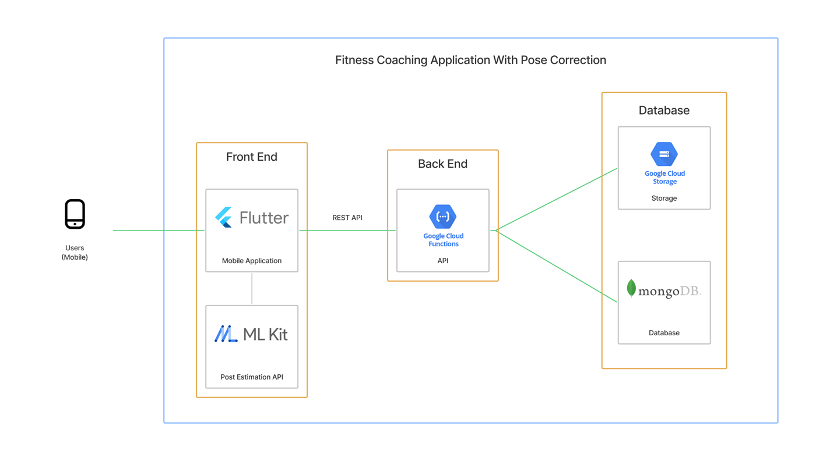
\includegraphics[width=\textwidth]{chapter_3/system overview}
    \caption{ภาพรวมระบบ}
\end{figure}

\section{แผนภาพยูสเคล (Use Case Diagram)}
\begin{figure}
    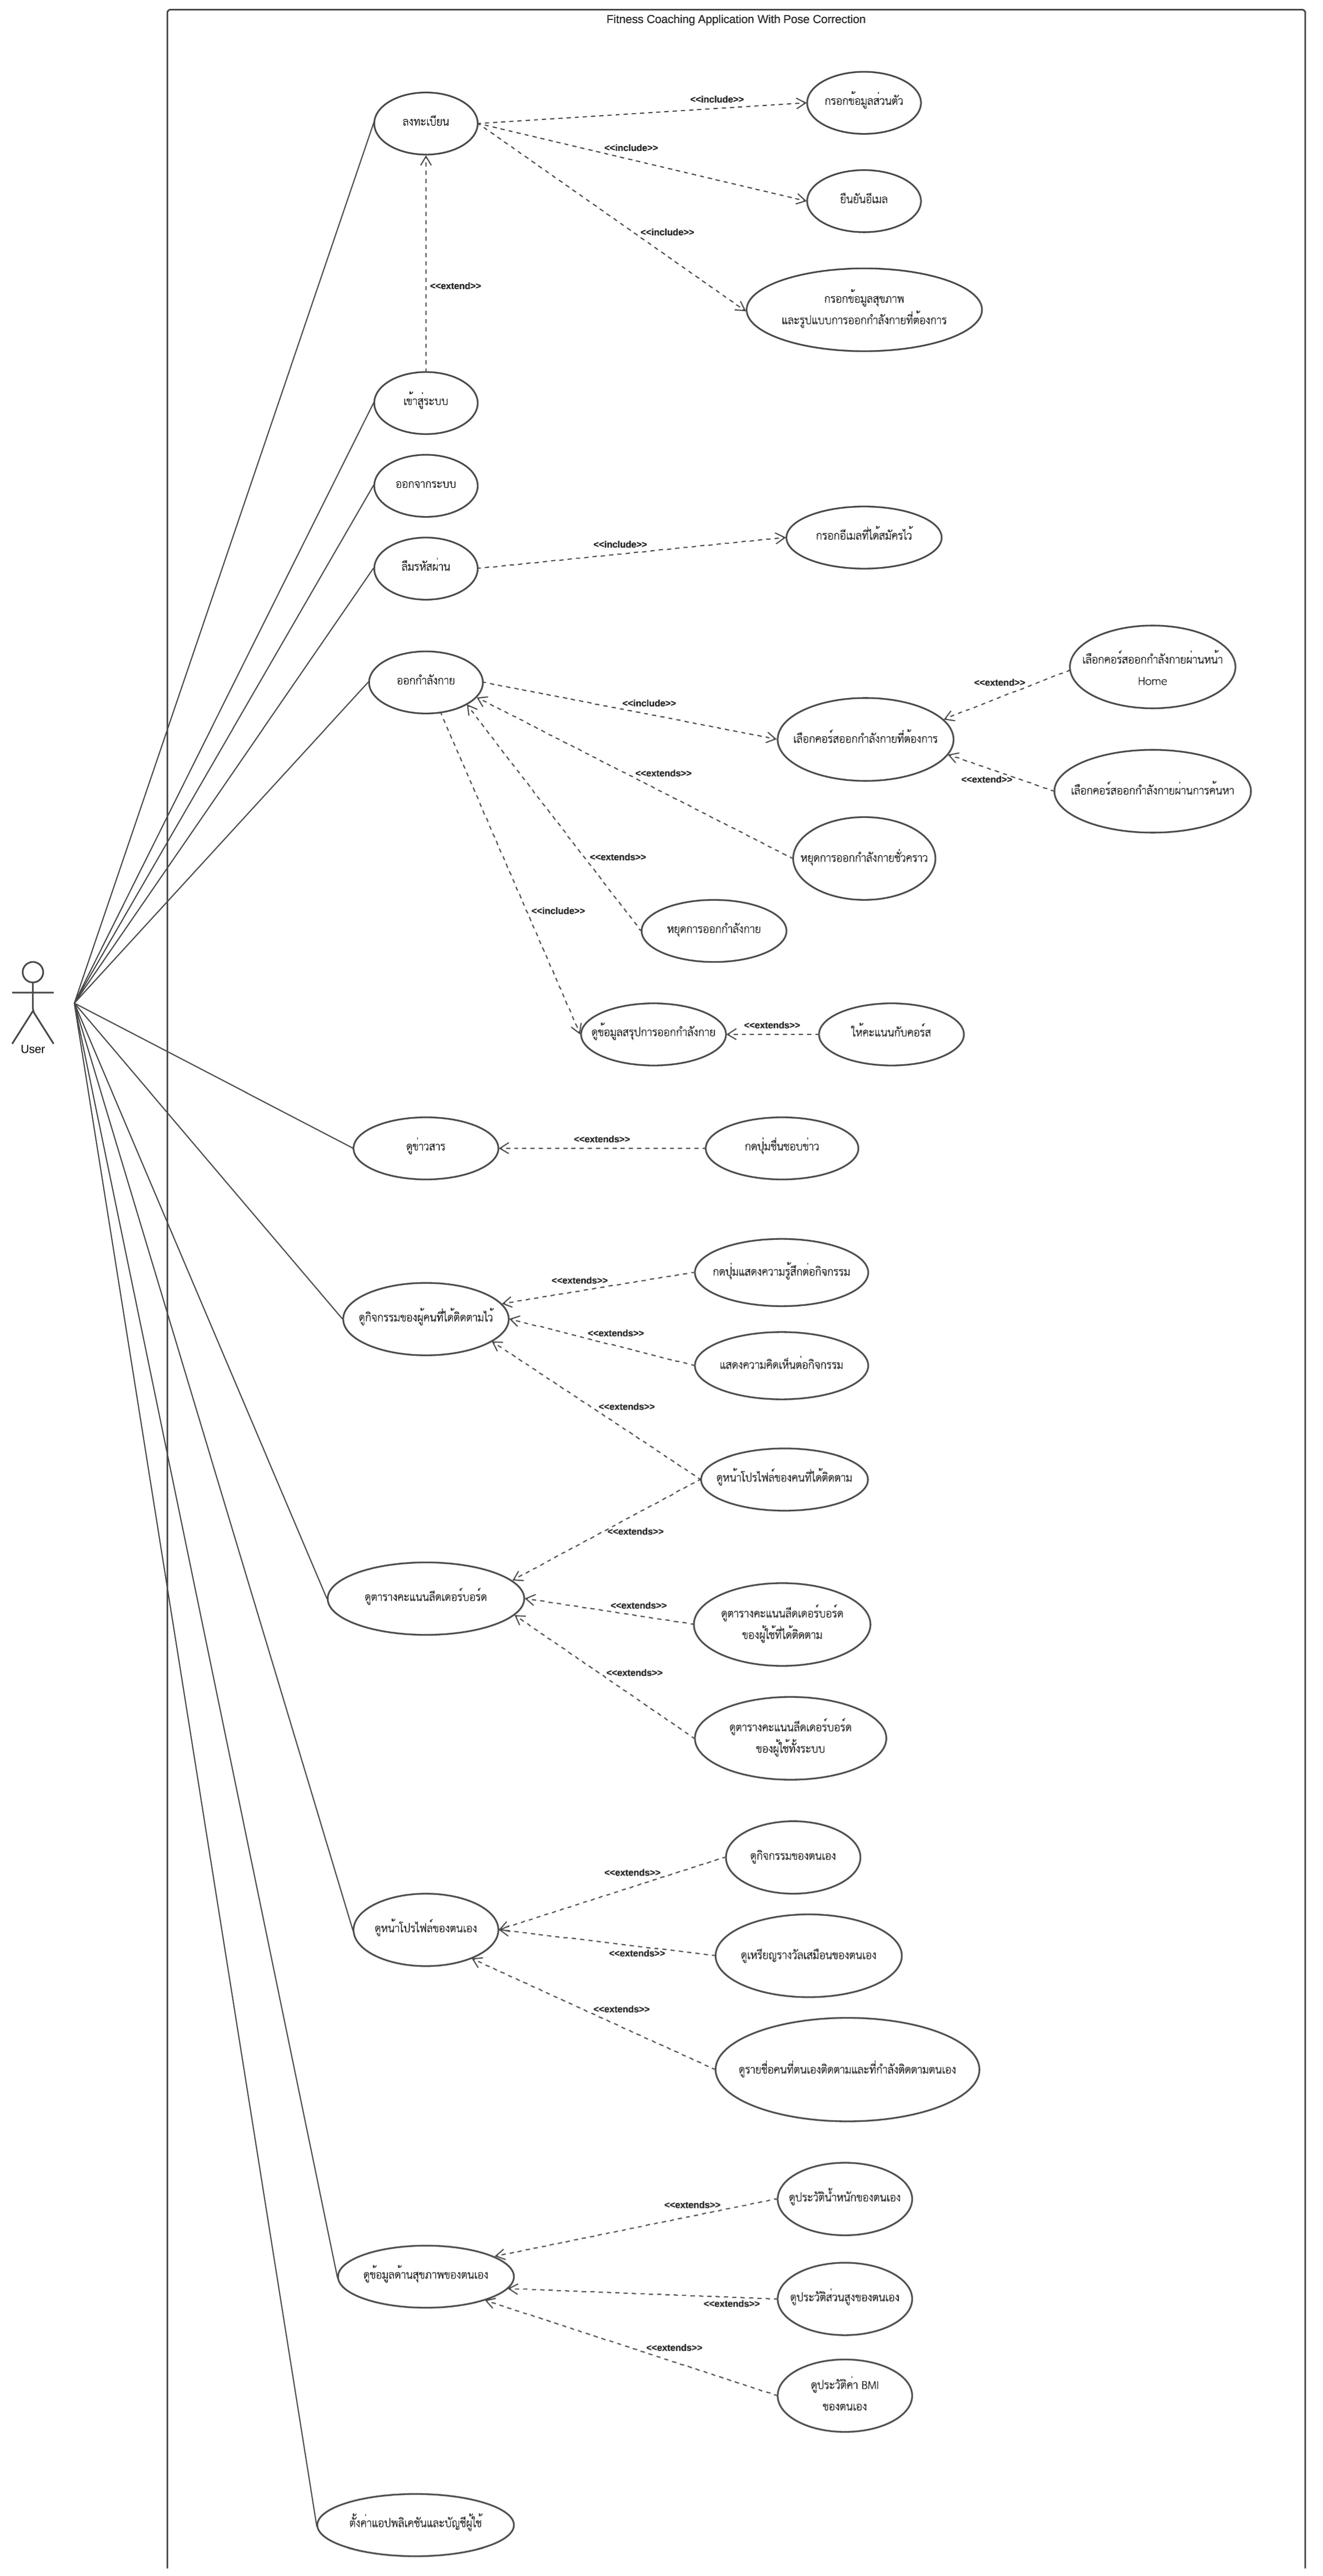
\includegraphics[height=\textheight - 3cm]{chapter_3/use case}
    \caption{แผนภาพยูสเคส}
\end{figure}
จากแผนภาพยูสเคสสามารถอธิบายได้ดังนี้
\begin{enumerate}
    \item ผู้ใช้สามารถลงทะเบียนเข้าใช้งานแอปพลิเคชันได้
    \item ผู้ใช้สามารถเข้าสู่ระบบได้
    \item ผู้ใช้สามารถออกจากระบบได้
    \item ผู้ใช้สามารถทำการกดลืมรหัสผ่านเพื่อตั้งค่ารหัสผ่านใหม่ได้
    \item ผู้ใช้สามารถเข้าสู่การออกกำลังกายได้
    \item ผู้ใช้สามารถดูข่าวสารของแอปพลิเคชันได้
    \item ผู้ใช้สามารถดูกิจกรรมของผู้คนที่ได้ติดตามไว้ได้
    \item ผู้ใช้สามารถดูตารางคะแนนลีดเดอร์บอร์ดได้
    \item ผู้ใช้สามารถดูหน้าโปรไฟล์ของตนเองได้
    \item ผู้ใช้สามารถดูข้อมูลด้านสุขภาพของตนเองได้
    \item ผู้ใช้สามารถตั้งค่าแอปพลิเคชันและตั้งค่าบัญชีผู้ใช้ได้
\end{enumerate}
\clearpage

\begin{table}
    \caption{รายละเอียด ลงทะเบียน}
    \begin{tabularx}{\textwidth}{ | >{\centering\bf} p{3cm} | X |}
        \hline
        Use Case: & ลงทะเบียน \\\hline
        Actor: & ผู้ใช้ \\\hline
        Main Flow: &
            \begin{enumerate}[table]
                \item ผู้ใช้ทำการกรอก email
                \item ผู้ใช้ทำการกรอก password ที่ต้องการ
                \item ผู้ใช้ทำการกรอก password เพื่อยืนยันอีกครั้ง
                \item ผู้ใช้ตรวจสอบการ verify email ที่ email ของตนเอง
                \item ผู้ใช้ทำการกรอก display name ที่ต้องการ
                \item ผู้ใช้ทำการเพิ่ม profile picture (สามารถข้ามได้)
            \end{enumerate}\\\hline
        Exception Flow: &
            \begin{enumerate}[table]
                \item กรณีผู้ใช้ทำการกรอก email ไม่ถูกต้องตามรูปแบบที่กำหนด แอปพลิเคชันจะแสดงข้อความว่า “Please enter a valid email”
                \item กรณีผู้ใช้ทำการกรอก password ทั้งสองช่องไม่ตรงกัน แอปพลิเคชันจะแสดงข้อความว่า “Please confirm your password”
                \item กรณีผู้ใช้ทำการกรอก password ไม่ถูกต้องตามที่เงื่อนไขกำหนด แอปพลิเคชันจะแสดงข้อความว่า “Your password must be at least 6 characters long. Please try another.”
                \item กรณีผู้ใช้ทำการกรอก display name ที่ซ้ำกันในระบบ แอปพลิเคชันจะแสดงข้อความ “This display name is already exist.”
            \end{enumerate}\\\hline
    \end{tabularx}
\end{table}


\begin{table}
    \caption{รายละเอียด เข้าสู่ระบบ}
    \begin{tabularx}{\textwidth}{ | >{\centering\bf} p{3cm} | X |}
        \hline
        Use Case: & เข้าสู่ระบบ \\\hline
        Actor: & ผู้ใช้ \\\hline
        Pre-Condition: &
        \begin{enumerate}[table]
            \item ผู้ใช้ได้เชื่อมต่ออินเทอร์เน็ต
            \item ผู้ใช้ต้องมีบัญชีผู้ใช้อยู่ในระบบ
        \end{enumerate} \\\hline
        
        Main Flow: & 
        \begin{enumerate}[table]
            \item ผู้ใช้กรอก email และ password
            \item ผู้ใช้ทำการกดปุ่มเข้าสู่ระบบ
        \end{enumerate}\\\hline
        Exception Flow: & 
        \begin{enumerate}[table]
            \item กรณีผู้ใช้ทำการกรอก email ไม่ถูกต้องตามรูปแบบที่กำหนด แอปพลิเคชันจะแสดงข้อความว่า “Please enter a valid email”
        \end{enumerate}\\\hline
    \end{tabularx}
\end{table}


\begin{table}
    \caption{รายละเอียด ออกจากระบบ}
    \begin{tabularx}{\textwidth}{ | >{\centering\bf} p{3cm} | X |}
        \hline
        Use Case: & ออกจากระบบ \\\hline
        Actor: & ผู้ใช้ \\\hline
        Pre-Condition: &
        \begin{enumerate}[table]
            \item ผู้ใช้ได้เข้าสู่ระบบเรียบร้อยแล้ว
        \end{enumerate} \\\hline
        
        Main Flow: & 
        \begin{enumerate}[table]
            \item ผู้ใช้กดปุ่มออกจากระบบ
        \end{enumerate}\\\hline
    \end{tabularx}
\end{table}

\begin{table}
    \caption{รายละเอียด ลืมรหัสผ่าน}
    \begin{tabularx}{\textwidth}{ | >{\centering\bf} p{3cm} | X |}
        \hline
        Use Case: & ลืมรหัสผ่าน \\\hline
        Actor: & ผู้ใช้ \\\hline
        Pre-Condition: &
        \begin{enumerate}[table]
            \item ผู้ใช้ได้เชื่อมต่ออินเทอร์เน็ต
            \item ผู้ใช้ต้องมีบัญชีผู้ใช้อยู่ในระบบ
        \end{enumerate} \\\hline
        
        Main Flow: & 
        \begin{enumerate}[table]
            \item ผู้ใช้กรอก email ที่ได้ทำการลงทะเบียนไว้
            \item แอปพลิเคชันส่งอีเมลเพื่อ reset รหัสผ่านไปยังผู้ใช้
            \item ผู้ใช้คลิกลิงค์เพื่อกำหนดรหัสผ่านใหม่
        \end{enumerate}\\\hline
        Exception Flow: & 
        \begin{enumerate}[table]
            \item กรณีผู้ใช้ทำการกรอก password ทั้งสองช่องไม่ตรงกัน แอปพลิเคชันจะแสดงข้อความว่า “Please confirm your password”
            \item กรณีผู้ใช้ทำการกรอก password ไม่ถูกต้องตามที่เงื่อนไขกำหนด แอปพลิเคชันจะแสดงข้อความว่า “Your password must be at least 6 characters long. Please try another.”
        \end{enumerate}\\\hline
    \end{tabularx}
\end{table}


\begin{table}
    \caption{รายละเอียด ออกกำลังกาย}
    \begin{tabularx}{\textwidth}{ | >{\centering\bf} p{3cm} | X |}
        \hline
        Use Case: & ออกกำลังกาย \\\hline
        Actor: & ผู้ใช้ \\\hline
        Pre-Condition: &
        \begin{enumerate}[table]
            \item ผู้ใช้ได้เข้าสู่ระบบเรียบร้อยแล้ว
        \end{enumerate} \\\hline
        
        Main Flow: & 
        \begin{enumerate}[table]
            \item ผู้ใช้กดเข้าหน้าหลักหรือค้นหาคอร์สออกกำลังกายเพื่อเลือกคอร์สออกกำลังกาย
            \item ผู้ใช้กดเลือกคอร์สออกกำลังกายที่ต้องการ
            \item ผู้ใช้วางโทรศัพท์มือถือ โดยให้กล้องหน้ามองเห็นร่างกายของผู้ใช้
            \item ผู้ใช้ออกกำลังกาย โดยทำตามท่าทางที่ทางแอปพลิเคชันได้สอนไว้
            \item ในระหว่างการออกกำลังกาย ผู้ใช้สามารถหยุดการออกกำลังกายชั่วคราว
            \item ในระหว่างการออกกำลังกาย ผู้ใช้สามารถหยุดการออกกำลังกาย
            \item เมื่อจบการออกกำลังกาย แอปพลิเคชันจะแสดงข้อมูลสรุปการออกกำลังกาย
            \item ผู้ใช้ให้คะแนนกับคอร์สออกกำลังกายที่ได้ออกไป
        \end{enumerate}\\\hline
        Exception Flow: & 
        \begin{enumerate}[table]
            \item เมื่อผู้ใช้ออกกำลังกายไม่ถูกต้อง แอปพลิเคชันจะมีเสียงแจ้งผู้ใช้ว่ากำลังออกกำลังกายไม่ถูกต้อง
        \end{enumerate}\\\hline
    \end{tabularx}
\end{table}


\begin{table}
    \caption{รายละเอียด หยุดการออกกำลังกายชั่วคราว}
    \begin{tabularx}{\textwidth}{ | >{\centering\bf} p{3cm} | X |}
        \hline
        Use Case: & หยุดการออกกำลังกายชั่วคราว \\\hline
        Actor: & ผู้ใช้ \\\hline
        Pre-Condition: &
        \begin{enumerate}[table]
            \item ผู้ใช้ได้เข้าสู่ระบบเรียบร้อยแล้ว
            \item ผู้ใช้อยู่ในหน้าการออกกำลังกาย
        \end{enumerate} \\\hline
        
        Main Flow: & 
        \begin{enumerate}[table]
            \item ผู้ใช้กดปุ่ม Pause เพื่อหยุดการออกกำลังกายชั่วคราว
            \item แอปพลิเคชันหยุดการจับเวลาการออกกำลังกายชั่วคราว
            \item ผู้ใช้กดปุ่ม Resume เพื่อเริ่มการออกกำลังกายต่อ
        \end{enumerate}\\\hline
    \end{tabularx}
\end{table}

\begin{table}
    \caption{รายละเอียด หยุดการออกกำลังกาย}
    \begin{tabularx}{\textwidth}{ | >{\centering\bf} p{3cm} | X |}
        \hline
        Use Case: & หยุดการออกกำลังกาย \\\hline
        Actor: & ผู้ใช้ \\\hline
        Pre-Condition: &
        \begin{enumerate}[table]
            \item ผู้ใช้ได้เข้าสู่ระบบเรียบร้อยแล้ว
            \item ผู้ใช้อยู่ในหน้าการออกกำลังกาย
        \end{enumerate} \\\hline
        
        Main Flow: & 
        \begin{enumerate}[table]
            \item ผู้ใช้กดปุ่ม Stop เพื่อหยุดการออกกำลังกาย หรือเมื่อผู้ใช้ออกกำลังกายเสร็จสิ้น
            \item แอปพลิเคชันหยุดการการออกกำลังกาย
        \end{enumerate}\\\hline
    \end{tabularx}
\end{table}

\begin{table}
    \caption{รายละเอียด ดูข่าวสาร}
    \begin{tabularx}{\textwidth}{ | >{\centering\bf} p{3cm} | X |}
        \hline
        Use Case: & ดูข่าวสาร \\\hline
        Actor: & ผู้ใช้ \\\hline
        Pre-Condition: &
        \begin{enumerate}[table]
            \item ผู้ใช้เข้าสู่ระบบเรียบร้อยแล้ว
        \end{enumerate} \\\hline
        
        Main Flow: & 
        \begin{enumerate}[table]
            \item ผู้ใช้กดปุ่มเลือกเข้าสู่หน้า News
            \item แอปพลิเคชันแสดงข้อมูลข่าวสาร
            \item ผู้ใช้เลือกอ่านข้อมูลข่าวสารที่เกี่ยวข้องกับการออกกำลังกาย ตามต้องการ
        \end{enumerate}\\\hline
    \end{tabularx}
\end{table}


\begin{table}
    \caption{รายละเอียด กดปุ่มชื่นชอบข่าว}
    \begin{tabularx}{\textwidth}{ | >{\centering\bf} p{3cm} | X |}
        \hline
        Use Case: & ดูข่าวสาร \\\hline
        Actor: & ผู้ใช้ \\\hline
        Pre-Condition: &
        \begin{enumerate}[table]
            \item ผู้ใช้ได้เข้าสู่ระบบเรียบร้อยแล้ว
            \item ผู้ใช้อยู่หน้าอ่านข้อมูลข่าวสาร          
        \end{enumerate} \\\hline
        
        Main Flow: & 
        \begin{enumerate}[table]
            \item ผู้ใช้ดูข้อมูลข่าวสาร
            \item ผู้ใช้กดปุ่มชื่นชอบข่าวสาร      
        \end{enumerate}\\\hline
    \end{tabularx}
\end{table}


\begin{table}
    \caption{รายละเอียด ดูกิจกรรมของผู้คนที่ได้ติดตามไว้}
    \begin{tabularx}{\textwidth}{ | >{\centering\bf} p{3cm} | X |}
        \hline
        Use Case: & ดูกิจกรรมของผู้คนที่ได้ติดตามไว้ \\\hline
        Actor: & ผู้ใช้ \\\hline
        Pre-Condition: &
        \begin{enumerate}[table]
            \item ผู้ใช้เข้าสู่ระบบเรียบร้อยแล้ว         
        \end{enumerate} \\\hline
        
        Main Flow: & 
        \begin{enumerate}[table]
            \item ผู้ใช้กดปุ่มเลือกเข้าสู่หน้า Activity
            \item ผู้ใช้เลือกดูกิจกรรมของผู้ใช้ที่ได้ติดตามไว้
            \item ผู้ใช้สามารถกดปุ่มแสดงความรู้สึกต่อกิจกรรม
            \item ผู้ใช้สามารถแสดงความคิดเห็นต่อกิจกรรม
            \item ผู้ใช้สามารถดูหน้าโปรไฟล์ของผู้ใช้ที่ได้ติดตามไว้
        \end{enumerate}\\\hline
    \end{tabularx}
\end{table}


\begin{table}
    \caption{รายละเอียด กดปุ่มแสดงความรู้สึกต่อกิจกรรม}
    \begin{tabularx}{\textwidth}{ | >{\centering\bf} p{3cm} | X |}
        \hline
        Use Case: & กดปุ่มแสดงความรู้สึกต่อกิจกรรม \\\hline
        Actor: & ผู้ใช้ \\\hline
        Pre-Condition: &
        \begin{enumerate}[table]
            \item ผู้ใช้ได้เข้าสู่ระบบเรียบร้อยแล้ว
            \item ผู้ใช้เลือกดูกิจกรรมของผู้ใช้ที่ได้ติดตามไว้
                   
        \end{enumerate} \\\hline
        
        Main Flow: & 
        \begin{enumerate}[table]
            \item ผู้ใช้กดปุ่มแสดงความรู้สึกต่อกิจกรรม
        \end{enumerate}\\\hline
    \end{tabularx}
\end{table}


\begin{table}
    \caption{รายละเอียด แสดงความคิดเห็นต่อกิจกรรม}
    \begin{tabularx}{\textwidth}{ | >{\centering\bf} p{3cm} | X |}
        \hline
        Use Case: & แสดงความคิดเห็นต่อกิจกรรม \\\hline
        Actor: & ผู้ใช้ \\\hline
        Pre-Condition: &
        \begin{enumerate}[table]
            \item ผู้ใช้ได้เข้าสู่ระบบเรียบร้อยแล้ว
            \item ผู้ใช้เลือกดูกิจกรรมของผู้ใช้ที่ได้ติดตามไว้      
        \end{enumerate} \\\hline
        
        Main Flow: & 
        \begin{enumerate}[table]
            \item ผู้ใช้กดแสดงความคิดเห็นต่อกิจกรรม
        \end{enumerate}\\\hline
    \end{tabularx}
\end{table}



\begin{table}
    \caption{รายละเอียด ดูตารางคะแนนลีดเดอร์บอร์ด}
    \begin{tabularx}{\textwidth}{ | >{\centering\bf} p{3cm} | X |}
        \hline
        Use Case: & ดูตารางคะแนนลีดเดอร์บอร์ด \\\hline
        Actor: & ผู้ใช้ \\\hline
        Pre-Condition: &
        \begin{enumerate}[table]
            \item ผู้ใช้ได้เข้าสู่ระบบเรียบร้อยแล้ว
            \item ผู้ใช้อยู่ในหน้า Activity
        \end{enumerate} \\\hline
        
        Main Flow: & 
        \begin{enumerate}[table]
            \item ผู้ใช้กดปุ่ม Leaderboard
            \item แอปพลิเคชันแสดงตารางคะแนนลีดเดอร์บอร์ด
            \item ผู้ใช้กดปุ่มเพื่อแสดงตารางคะแนนลีดเดอร์บอร์ดโดยจำแนกตามกลุ่มผู้ใช้ที่ได้ติดตามไว้ และกลุ่มผู้ใช้ทั้งระบบ
            \item ผู้ใช้สามารถกดดูหน้าโปรไฟล์ของผู้ใช้ที่ได้ติดตามไว้
        \end{enumerate}\\\hline
    \end{tabularx}
\end{table}



\begin{table}
    \caption{รายละเอียด ดูตารางคะแนนลีดเดอร์บอร์ดของผู้ใช้ที่ได้ติดตาม}
    \begin{tabularx}{\textwidth}{ | >{\centering\bf} p{3cm} | X |}
        \hline
        Use Case: & ดูตารางคะแนนลีดเดอร์บอร์ดของผู้ใช้ที่ได้ติดตาม \\\hline
        Actor: & ผู้ใช้ \\\hline
        Pre-Condition: &
        \begin{enumerate}[table]
            \item ผู้ใช้ได้เข้าสู่ระบบเรียบร้อยแล้ว
            \item ผู้ใช้อยู่ในหน้าแสดงตารางคะแนนลีดเดอร์บอร์ด         
        \end{enumerate} \\\hline
        
        Main Flow: & 
        \begin{enumerate}[table]
            \item ผู้ใช้กดปุ่มแสดงตารางคะแนนลีดเดอร์บอร์ดโดยจำแนกตามกลุ่มผู้ใช้ที่ได้ติดตามไว้
        \end{enumerate}\\\hline
    \end{tabularx}
\end{table}


\begin{table}
    \caption{รายละเอียด ดูตารางคะแนนลีดเดอร์บอร์ดของผู้ใช้ทั้งระบบ}
    \begin{tabularx}{\textwidth}{ | >{\centering\bf} p{3cm} | X |}
        \hline
        Use Case: & ดูตารางคะแนนลีดเดอร์บอร์ดของผู้ใช้ทั้งระบบ \\\hline
        Actor: & ผู้ใช้ \\\hline
        Pre-Condition: &
        \begin{enumerate}[table]
            \item ผู้ใช้ได้เข้าสู่ระบบเรียบร้อยแล้ว
            \item ผู้ใช้อยู่ในหน้าแสดงตารางคะแนนลีดเดอร์บอร์ด            
        \end{enumerate} \\\hline
        
        Main Flow: & 
        \begin{enumerate}[table]
            \item ผู้ใช้กดปุ่มแสดงตารางคะแนนลีดเดอร์บอร์ดโดยจำแนกตามกลุ่มผู้ใช้ทั้งระบบ
        \end{enumerate}\\\hline
    \end{tabularx}
\end{table}



\begin{table}
    \caption{รายละเอียด ดูหน้าโปรไฟล์ของตนเอง}
    \begin{tabularx}{\textwidth}{ | >{\centering\bf} p{3cm} | X |}
        \hline
        Use Case: & ดูหน้าโปรไฟล์ของตนเอง \\\hline
        Actor: & ผู้ใช้ \\\hline
        Pre-Condition: &
        \begin{enumerate}[table]
            \item ผู้ใช้ได้เข้าสู่ระบบเรียบร้อยแล้ว         
        \end{enumerate} \\\hline
        
        Main Flow: & 
        \begin{enumerate}[table]
            \item ผู้ใช้กดปุ่มเลือกเข้าสู่หน้า Profile
            \item แอปพลิเคชันแสดงข้อมูลสรุปของผู้ใช้
            \item ผู้ใช้ตรวจสอบกิจกรรมของตนเอง
            \item ผู้ใช้ตรวจสอบเหรียญรางวัลเสมือนของตนเอง
            \item ผู้ใช้ตรวจสอบรายชื่อการติดตามกับผู้ใช้อื่น
        \end{enumerate}\\\hline
    \end{tabularx}
\end{table}


\begin{table}
    \caption{รายละเอียด ดูกิจกรรมของตนเอง}
    \begin{tabularx}{\textwidth}{ | >{\centering\bf} p{3cm} | X |}
        \hline
        Use Case: & ดูกิจกรรมของตนเอง \\\hline
        Actor: & ผู้ใช้ \\\hline
        Pre-Condition: &
        \begin{enumerate}[table]
            \item ผู้ใช้ได้เข้าสู่ระบบเรียบร้อยแล้ว
            \item ผู้ใช้อยู่ในหน้า Profile 
        \end{enumerate} \\\hline
        
        Main Flow: & 
        \begin{enumerate}[table]
            \item ผู้ใช้กดปุ่มเลือกเข้าสู่หน้า Profile
            \item แอปพลิเคชันแสดงข้อมูลสรุปของผู้ใช้
            \item ผู้ใช้ตรวจสอบกิจกรรมของตนเอง
            \item ผู้ใช้ตรวจสอบเหรียญรางวัลเสมือนของตนเอง
            \item ผู้ใช้ตรวจสอบรายชื่อการติดตามกับผู้ใช้อื่น
        \end{enumerate}\\\hline
    \end{tabularx}
\end{table}


\begin{table}
    \caption{รายละเอียด ดูเหรียญรางวัลเสมือนของตนเอง}
    \begin{tabularx}{\textwidth}{ | >{\centering\bf} p{3cm} | X |}
        \hline
        Use Case: & ดูเหรียญรางวัลเสมือนของตนเอง \\\hline
        Actor: & ผู้ใช้ \\\hline
        Pre-Condition: &
        \begin{enumerate}[table]
            \item ผู้ใช้ได้เข้าสู่ระบบเรียบร้อยแล้ว
            \item ผู้ใช้อยู่ในหน้า Profile
            
        \end{enumerate} \\\hline
        
        Main Flow: & 
        \begin{enumerate}[table]
            \item ผู้ใช้กดปุ่มแสดงเหรียญรางวัลเสมือนของตนเอง
            \item ผู้ใช้ตรวจสอบเหรียญรางวัลเสมือนของตนเอง
        \end{enumerate}\\\hline
    \end{tabularx}
\end{table}


\begin{table}
    \caption{รายละเอียด ดูรายชื่อคนที่ตนเองติดตามและที่กำลังติดตามตนเอง}
    \begin{tabularx}{\textwidth}{ | >{\centering\bf} p{3cm} | X |}
        \hline
        Use Case: & ดูรายชื่อคนที่ตนเองติดตามและที่กำลังติดตามตนเอง \\\hline
        Actor: & ผู้ใช้ \\\hline
        Pre-Condition: &
        \begin{enumerate}[table]
            \item ผู้ใช้ได้เข้าสู่ระบบเรียบร้อยแล้ว
            \item ผู้ใช้อยู่ในหน้า Profile
        \end{enumerate} \\\hline
        
        Main Flow: & 
        \begin{enumerate}[table]
            \item ผู้ใช้กดข้อความ Follower เพื่อตรวจสอบรายชื่อคนที่กำลังติดตามตนเอง
            \item ผู้ใช้กดข้อความ Following เพื่อตรวจสอบรายชื่อคนที่ตนเองติดตาม
            \item แอปพลิเคชันแสดงรายชื่อคนที่ตนเองติดตามและที่กำลังติดตามตนเอง
            \item ผู้ใช้ตรวจสอบรายชื่อคนที่ตนเองติดตามและที่กำลังติดตามตนเอง
        \end{enumerate} \\\hline
    \end{tabularx}
\end{table}


\begin{table}
    \caption{รายละเอียด ดูข้อมูลด้านสุขภาพของตนเอง}
    \begin{tabularx}{\textwidth}{ | >{\centering\bf} p{3cm} | X |}
        \hline
        Use Case: & ดูข้อมูลด้านสุขภาพของตนเอง \\\hline
        Actor: & ผู้ใช้ \\\hline
        Pre-Condition: &
        \begin{enumerate}[table]
            \item ผู้ใช้ได้เข้าสู่ระบบเรียบร้อยแล้ว
            \item ผู้ใช้อยู่ในหน้า Profile            
        \end{enumerate} \\\hline
        
        Main Flow: & 
        \begin{enumerate}[table]
            \item ผู้ใช้กดปุ่ม Health Stats
            \item แอปพลิเคชันแสดงหน้า Health Stats ซึ่งแสดงข้อมูลด้านสุขภาพ (จำนวนนาทีการออกกำลังกาย, น้ำหนัก, ส่วนสูง, ค่า BMI) ของตนเอง
            \item ผู้ใช้ตรวจสอบข้อมูลด้านสุขภาพของตนเอง  
        \end{enumerate}\\\hline
    \end{tabularx}
\end{table}


\begin{table}
    \caption{รายละเอียด ดูประวัติน้ำหนักของตนเอง}
    \begin{tabularx}{\textwidth}{ | >{\centering\bf} p{3cm} | X |}
        \hline
        Use Case: & ดูประวัติน้ำหนักของตนเอง \\\hline
        Actor: & ผู้ใช้ \\\hline
        Pre-Condition: &
        \begin{enumerate}[table]
            \item ผู้ใช้ได้เข้าสู่ระบบเรียบร้อยแล้ว
            \item ผู้ใช้อยู่ในหน้า Health Stats          
        \end{enumerate} \\\hline
        
        Main Flow: & 
        \begin{enumerate}[table]
            \item ผู้ใช้กดปุ่ม Weight
            \item แอปพลิเคชันแสดงข้อมูลสถิติของค่าน้ำหนักของผู้ใช้ที่ได้บันทึกไว้ โดยแสดงเป็นกราฟเส้นและค่าที่ได้บันทึกไว้
            \item ผู้ใช้ตรวจสอบสถิติค่าน้ำหนักของตนเอง
        \end{enumerate}\\\hline
    \end{tabularx}
\end{table}



\begin{table}
    \caption{รายละเอียด ดูประวัติส่วนสูงของตนเอง}
    \begin{tabularx}{\textwidth}{ | >{\centering\bf} p{3cm} | X |}
        \hline
        Use Case: & ดูประวัติส่วนสูงของตนเอง \\\hline
        Actor: & ผู้ใช้ \\\hline
        Pre-Condition: &
        \begin{enumerate}[table]
            \item ผู้ใช้ได้เข้าสู่ระบบเรียบร้อยแล้ว
            \item ผู้ใช้อยู่ในหน้า Health Stats          
        \end{enumerate} \\\hline
        
        Main Flow: & 
        \begin{enumerate}[table]
            \item ผู้ใช้กดปุ่ม Height
            \item แอปพลิเคชันแสดงข้อมูลสถิติของค่าส่วนสูงของผู้ใช้ที่ได้บันทึกไว้ โดยแสดงเป็นกราฟเส้นและค่าที่ได้บันทึกไว้
            \item ผู้ใช้ตรวจสอบสถิติค่าส่วนสูงของตนเอง   
        \end{enumerate}\\\hline
    \end{tabularx}
\end{table}


\begin{table}
    \caption{รายละเอียด ดูประวัติค่า BMI ของตนเอง}
    \begin{tabularx}{\textwidth}{ | >{\centering\bf} p{3cm} | X |}
        \hline
        Use Case: & ดูประวัติค่า BMI ของตนเอง \\\hline
        Actor: & ผู้ใช้ \\\hline
        Pre-Condition: &
        \begin{enumerate}[table]
            \item ผู้ใช้ได้เข้าสู่ระบบเรียบร้อยแล้ว
            \item ผู้ใช้อยู่ในหน้า Health Stats
        \end{enumerate} \\\hline
        
        Main Flow: & 
        \begin{enumerate}[table]
            \item ผู้ใช้กดปุ่ม BMI
            \item แอปพลิเคชันแสดงข้อมูลสถิติของค่า BMI ของผู้ใช้ที่แอปพลิเคชันคำนวณมาจากค่าน้ำหนักและส่วนสูงที่ผู้ใช้ได้บันทึกไว้
            \item ผู้ใช้ตรวจสอบสถิติค่า BMI ของตนเอง
        \end{enumerate}\\\hline
    \end{tabularx}
\end{table}



\begin{table}
    \caption{รายละเอียด ตั้งค่าแอปพลิเคชันและบัญชีผู้ใช้}
    \begin{tabularx}{\textwidth}{ | >{\centering\bf} p{3cm} | X |}
        \hline
        Use Case: & ตั้งค่าแอปพลิเคชันและบัญชีผู้ใช้ \\\hline
        Actor: & ผู้ใช้ \\\hline
        Pre-Condition: &
        \begin{enumerate}[table]
            \item ผู้ใช้ได้เข้าสู่ระบบเรียบร้อยแล้ว
            \item ผู้ใช้อยู่ในหน้า Profile            
        \end{enumerate} \\\hline
        
        Main Flow: & 
        \begin{enumerate}[table]
            \item ผู้ใช้กดปุ่ม Settings
            \item แอปพลิเคชันแสดงหน้า Settings ในการตั้งค่าแอปพลิเคชันและบัญชีผู้ใช้
            \item ผู้ใช้ตรวจสอบการตั้งค่าแอปพลิเคชันและบัญชีผู้ใช้
            \item ผู้ใช้กำหนดค่าของการตั้งค่าแอปพลิเคชันและบัญชีผู้ใช้            
        \end{enumerate}\\\hline
    \end{tabularx}
\end{table}
\clearpage

\section{แผนผังการทำงานแบบลำดับปฏิสัมพันธ์ (Sequence Diagram)}
การออกแบบแผนผังการทำงานแบบลำดับปฏิสัมพันธ์ ดังนี้

\begin{figure}
    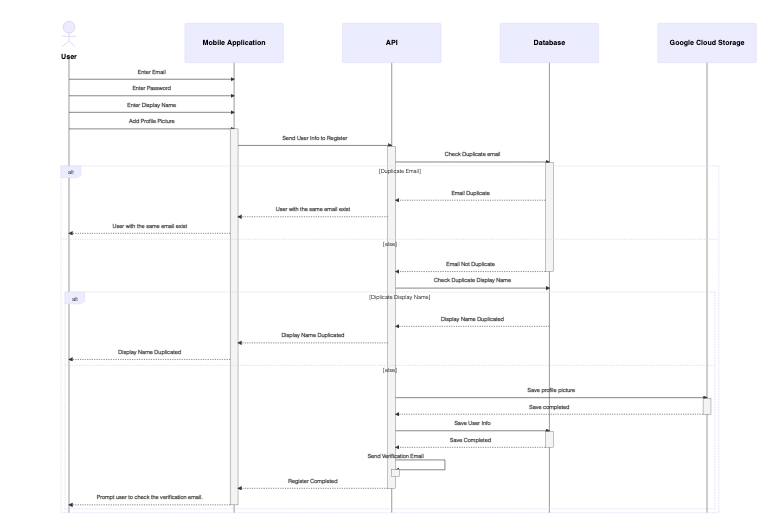
\includegraphics[width=\textwidth]{chapter_3/sequence/Register-1.md.png}
    \caption{การทำงานในส่วนการลงทะเบียนผู้ใช้}
\end{figure}

\begin{figure}
    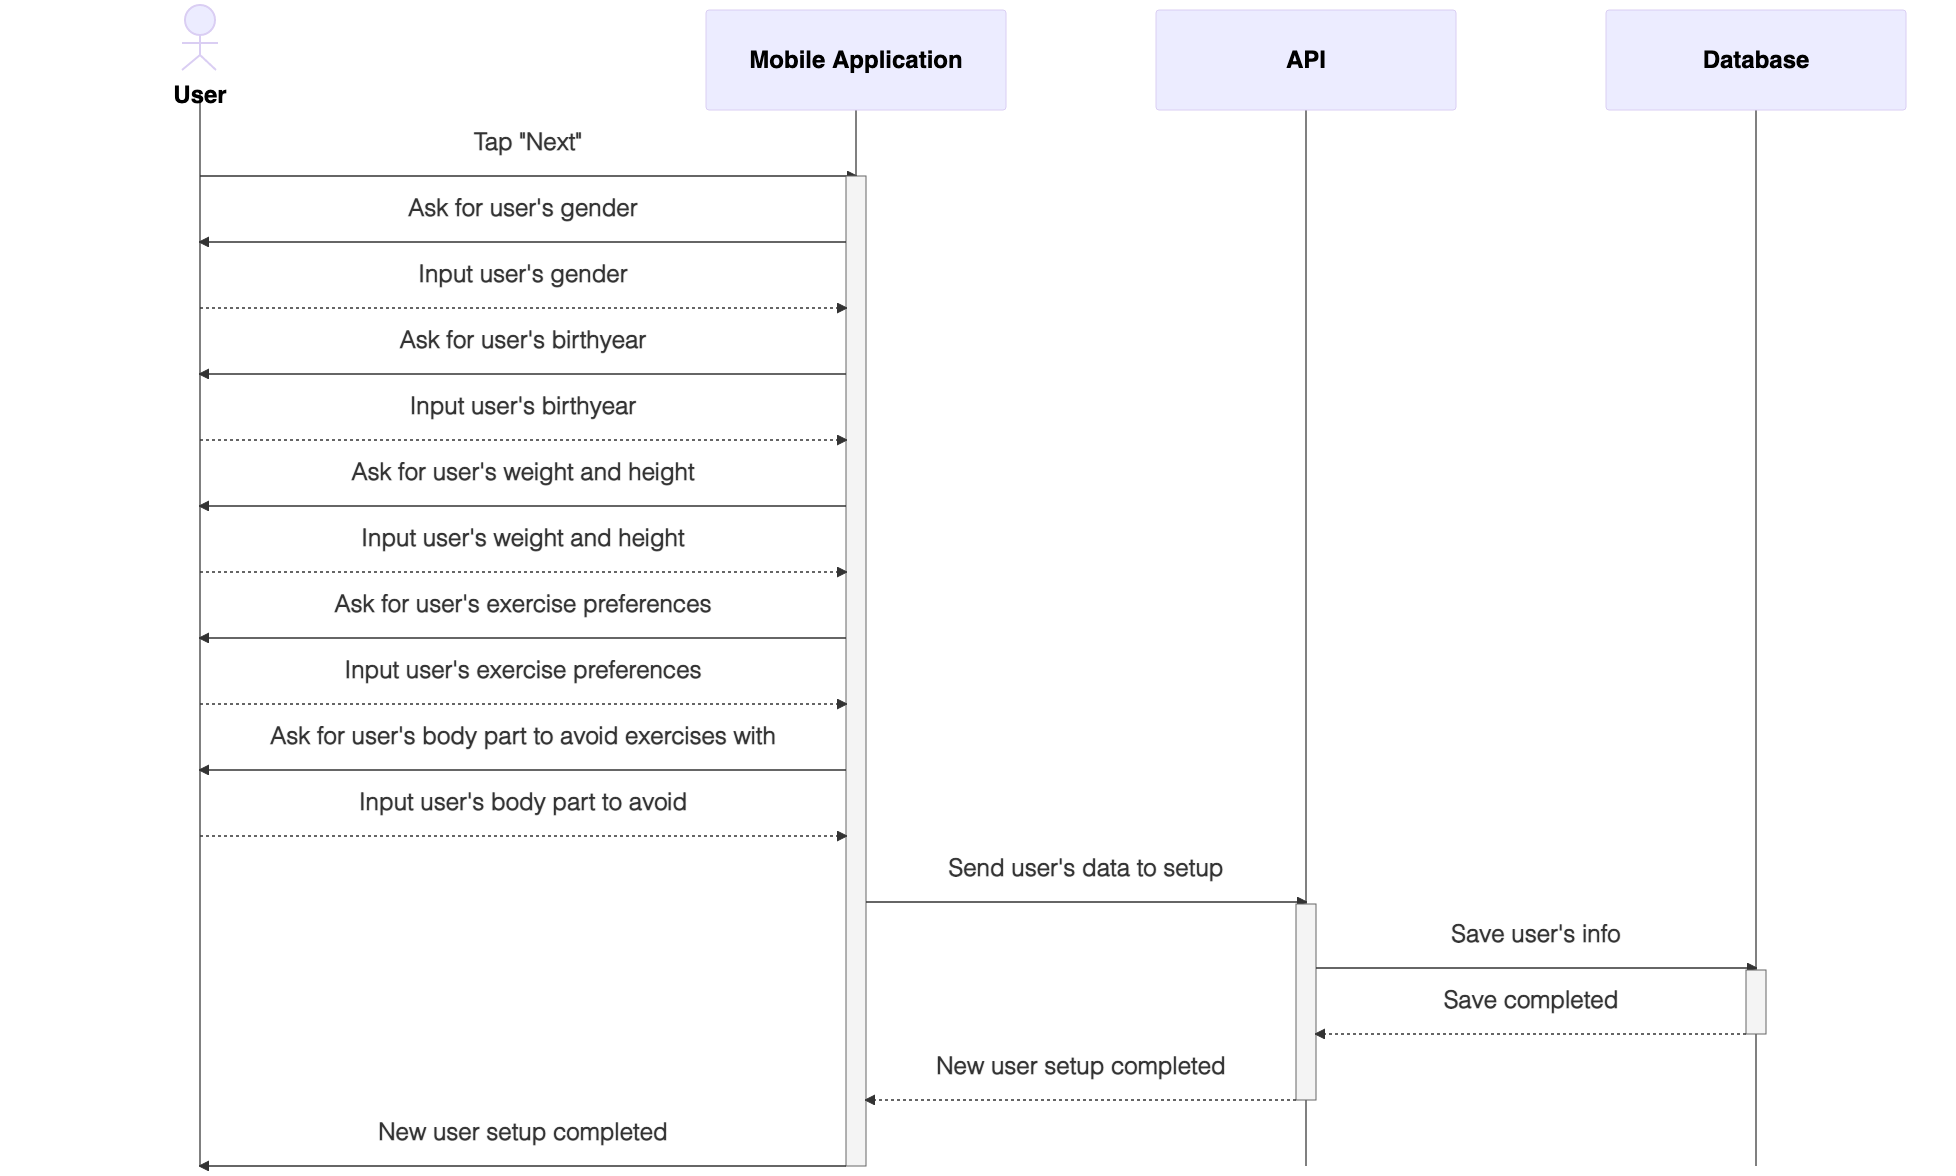
\includegraphics[width=\textwidth]{chapter_3/sequence/New User Setup-1.md.png}
    \caption{การทำงานในส่วนการตอบคำถามความต้องการออกกำลังกาย}
\end{figure}

\begin{figure}
    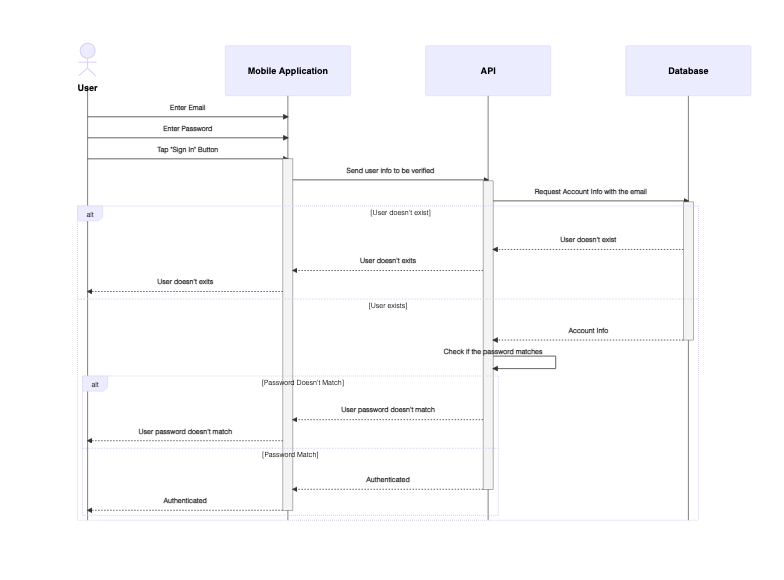
\includegraphics[width=\textwidth]{chapter_3/sequence/Sign In-1.md.png}
    \caption{การทำงานในส่วนการเข้าสู่ระบบ}
\end{figure}

\begin{figure}
    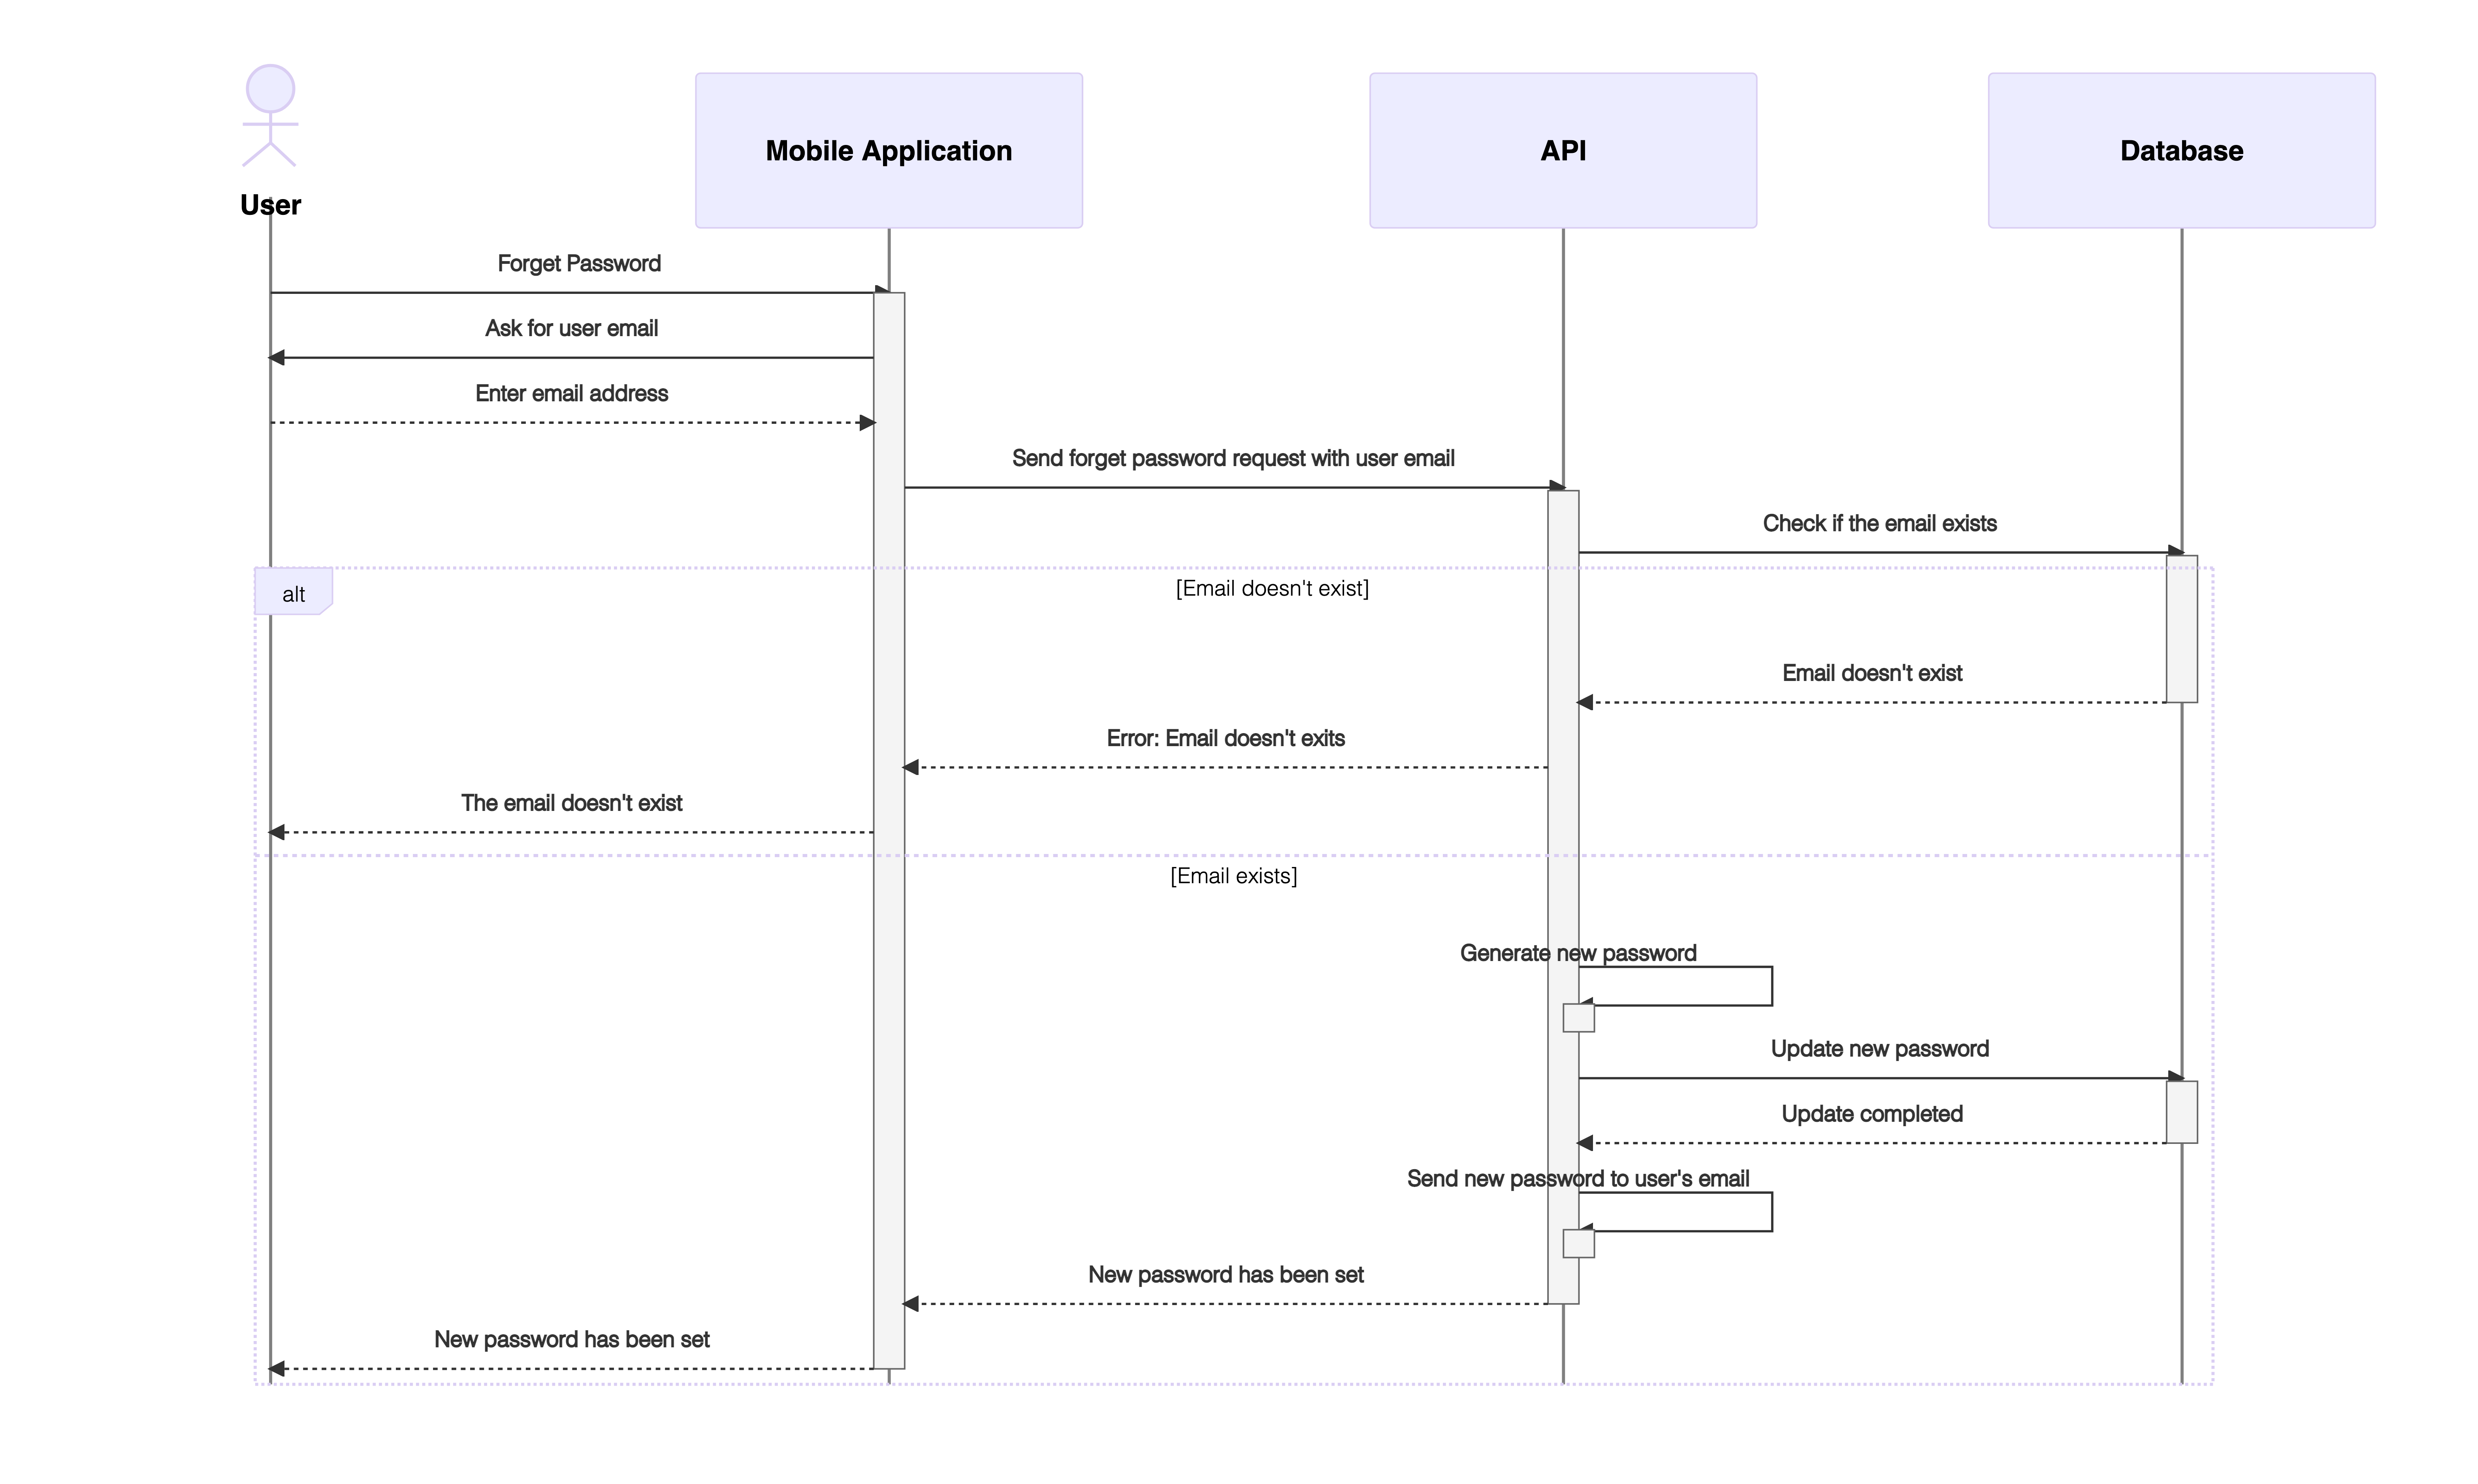
\includegraphics[width=\textwidth]{chapter_3/sequence/Forget Password-1.md.png}
    \caption{การทำงานในส่วนการลืมรหัสผ่าน}
\end{figure}

\begin{figure}
    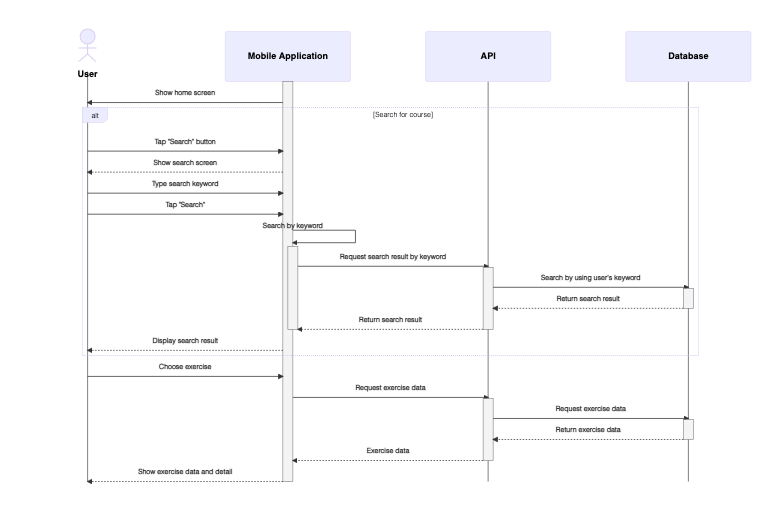
\includegraphics[width=\textwidth]{chapter_3/sequence/Exercise Course Selection-1.md.png}
    \caption{การทำงานในส่วนการเลือกคอร์สออกกำลังกาย}
\end{figure}

\begin{figure}
    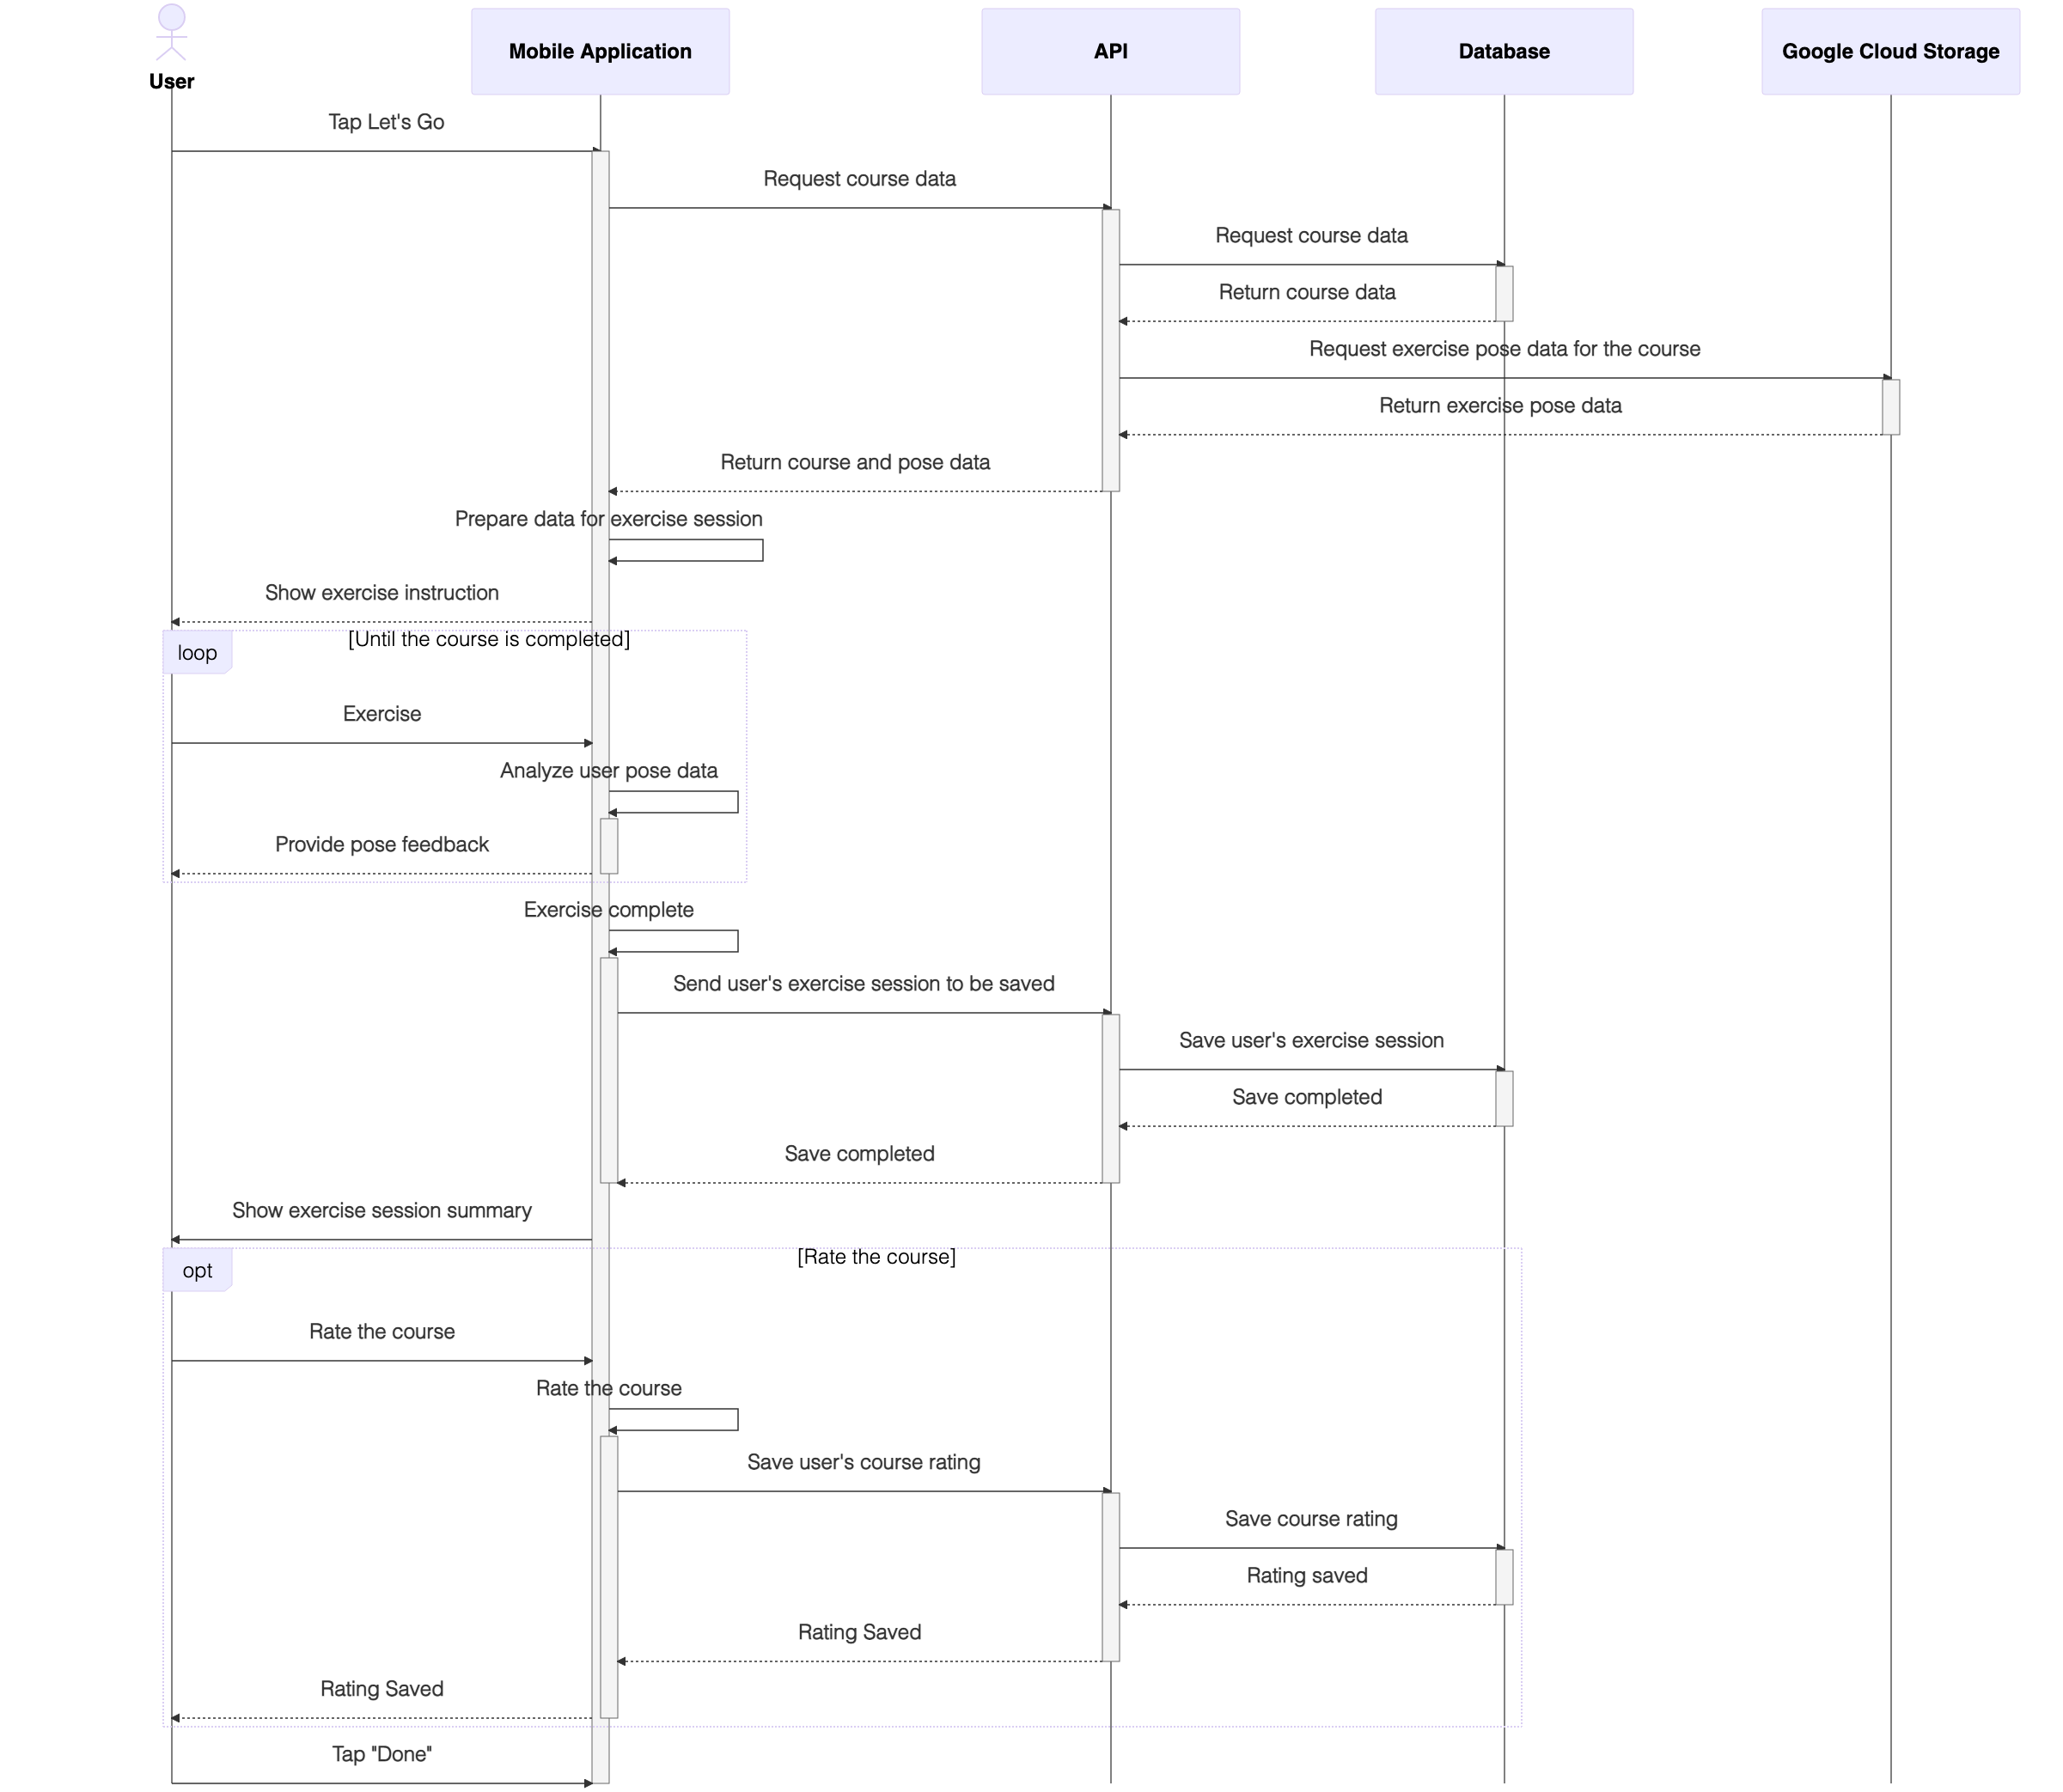
\includegraphics[width=\textwidth]{chapter_3/sequence/Exercise-1.md.png}
    \caption{การทำงานในส่วนการออกกำลังกาย}
\end{figure}

\begin{figure}
    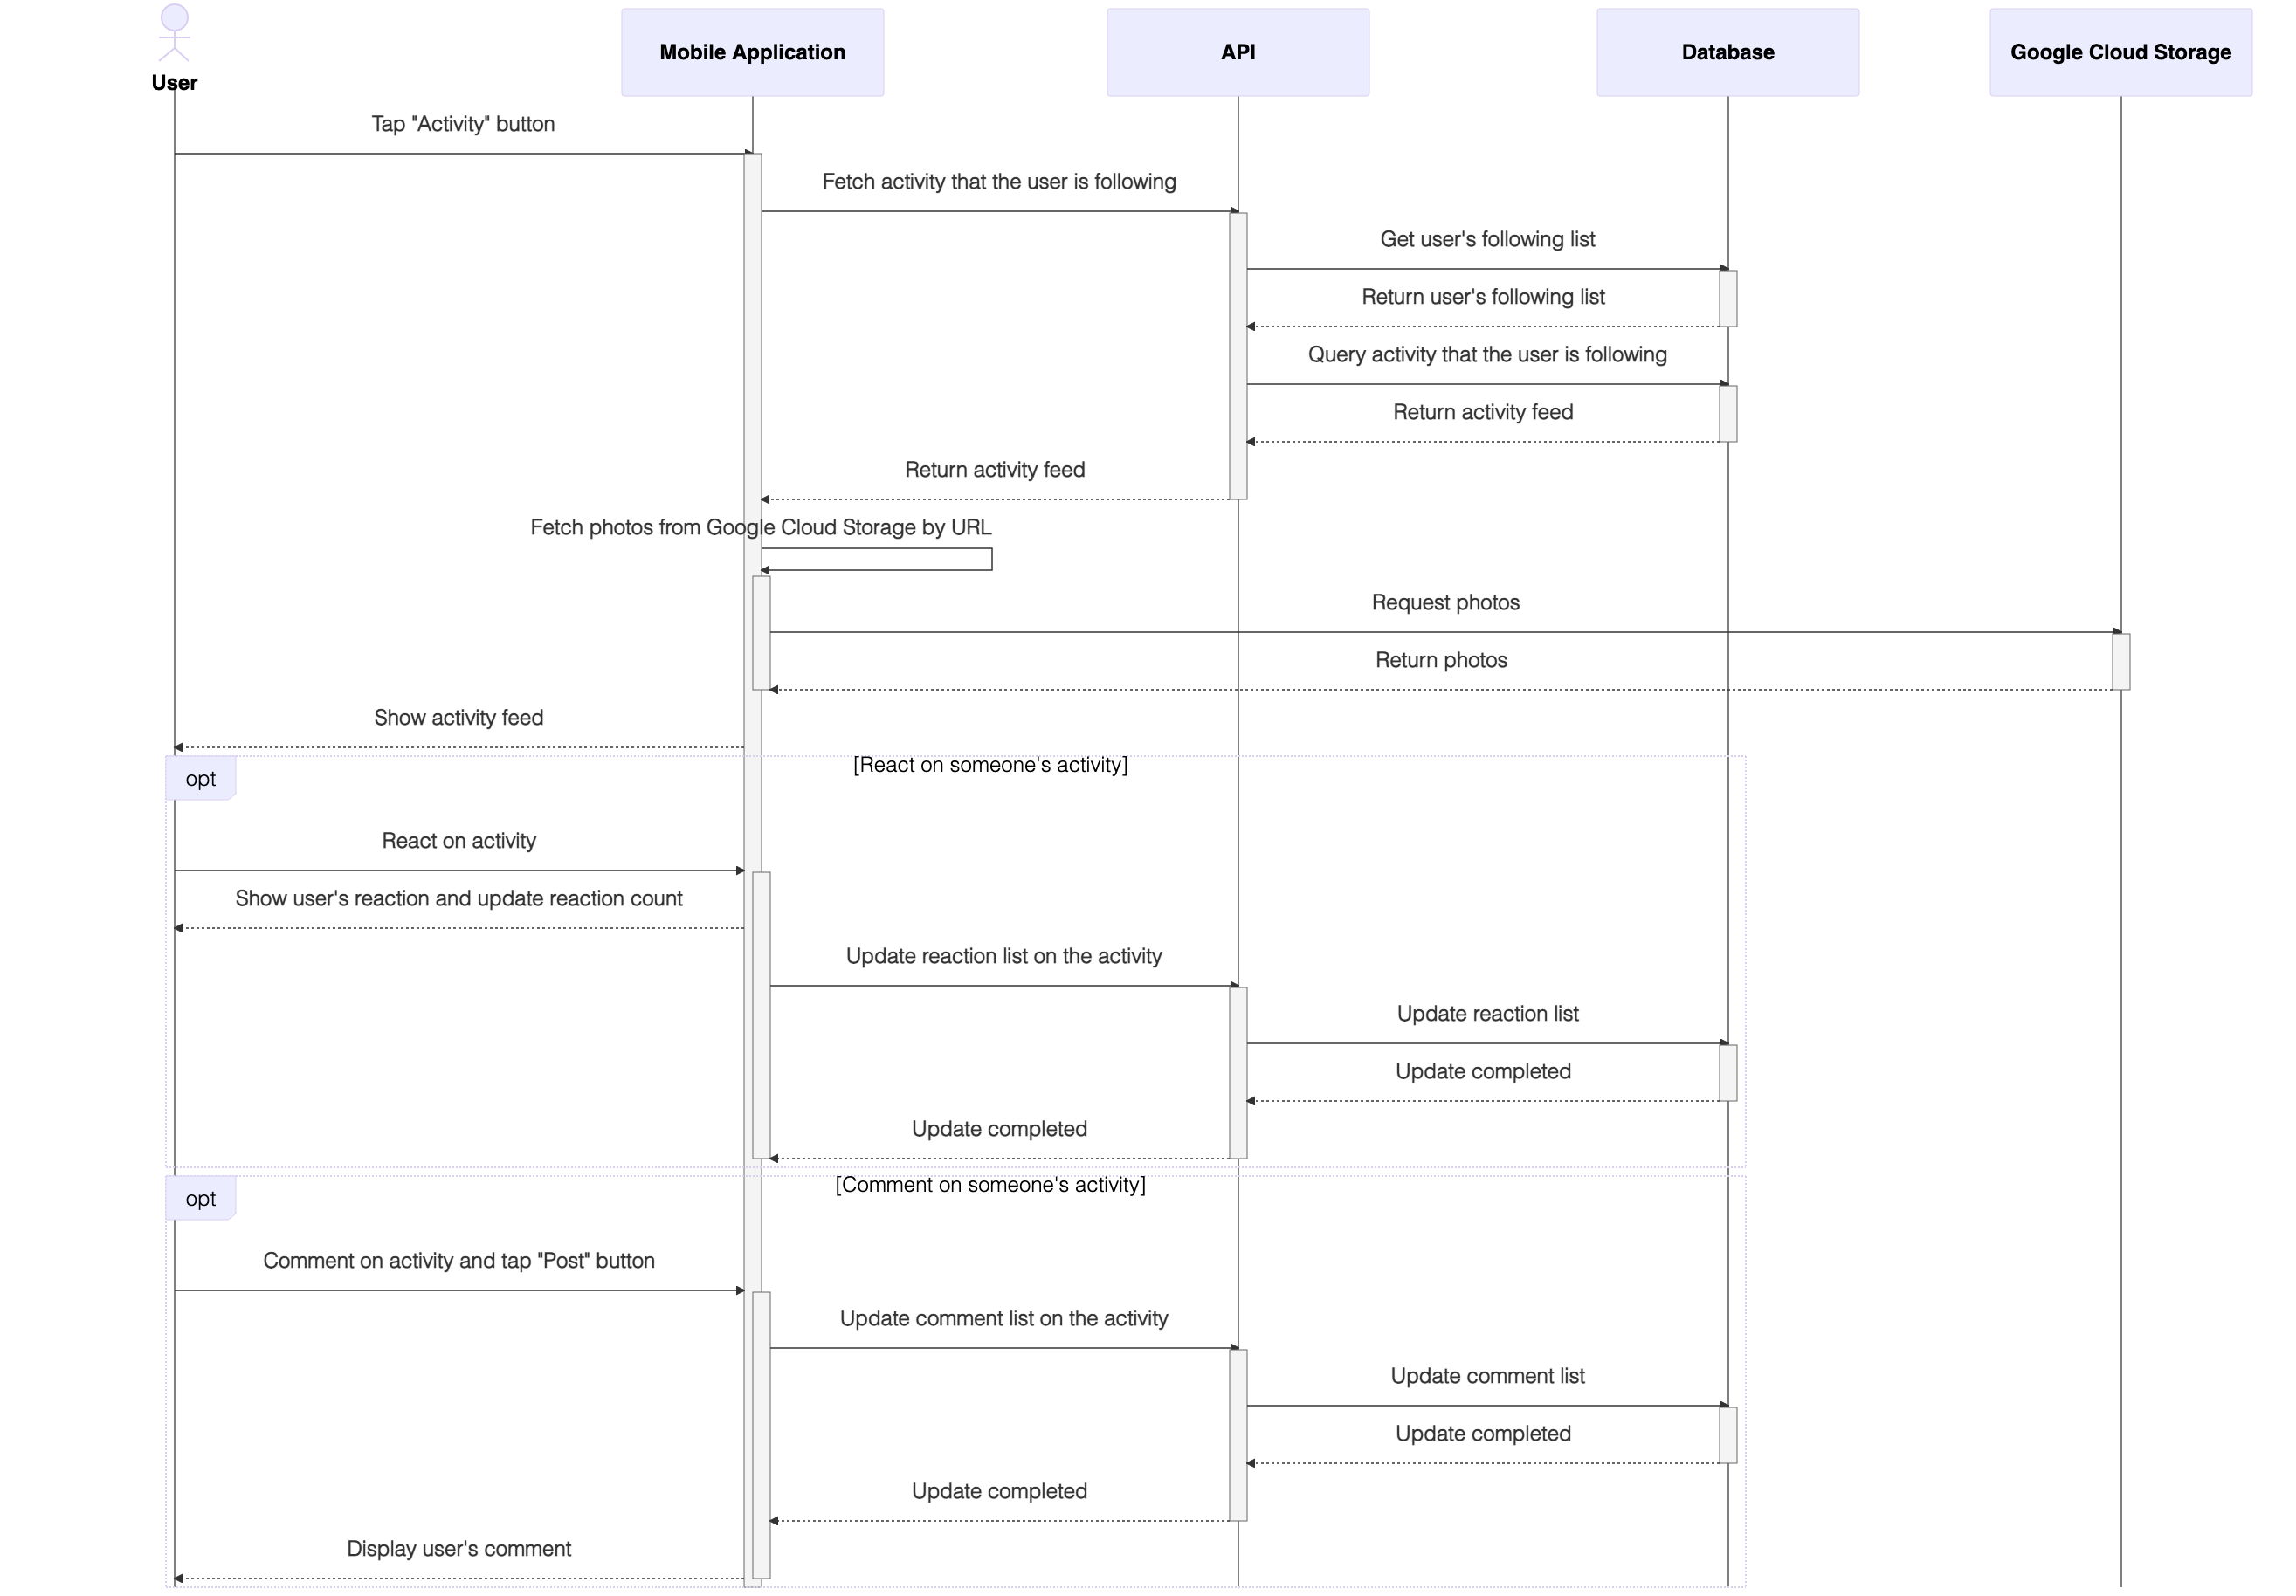
\includegraphics[width=\textwidth]{chapter_3/sequence/Activity-1.md.png}
    \caption{การทำงานในส่วนกิจกรรมของผู้ใช้}
\end{figure}

\begin{figure}
    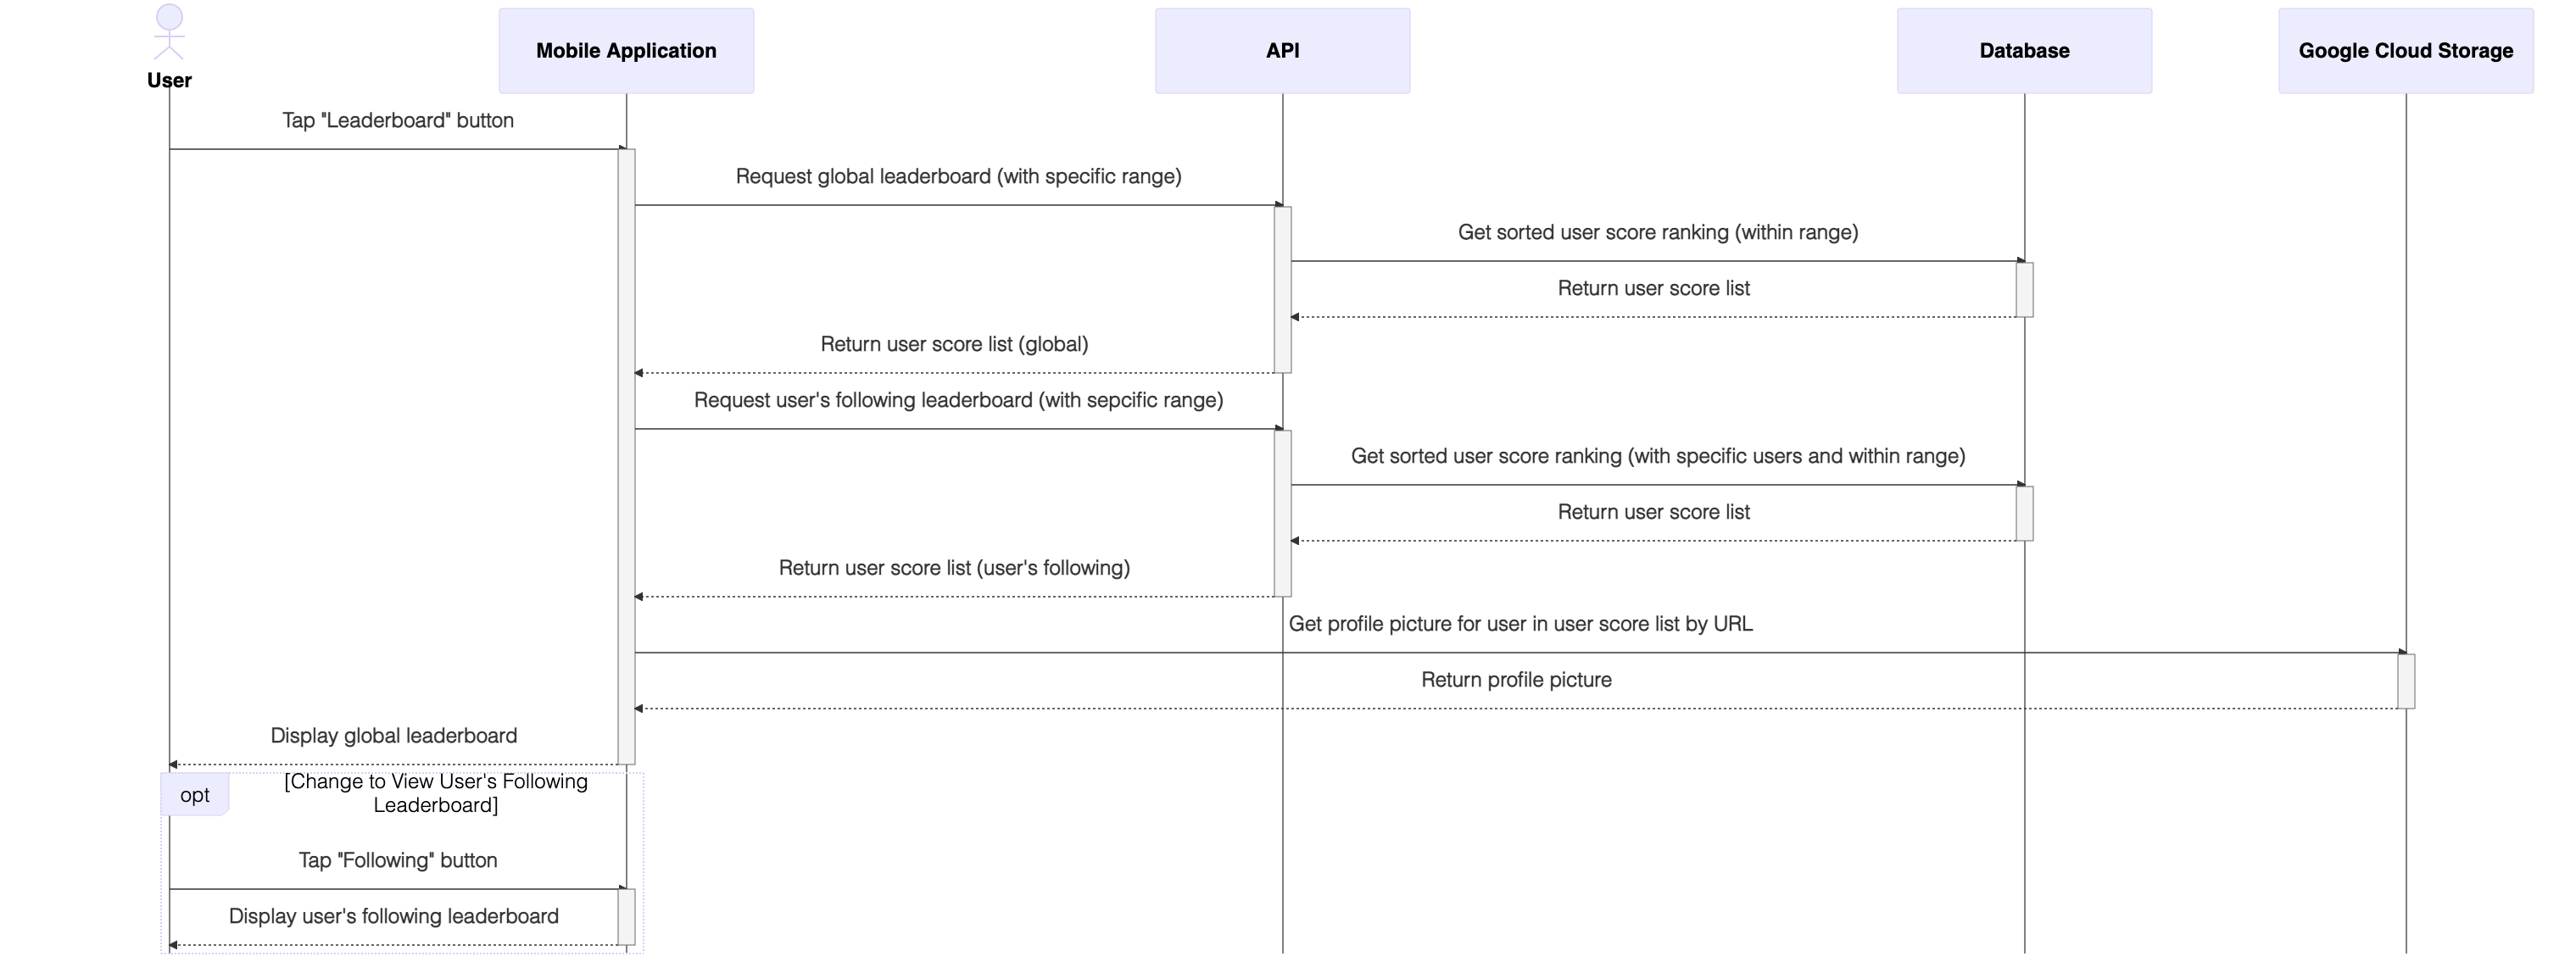
\includegraphics[width=\textwidth]{chapter_3/sequence/Leaderboard-1.md.png}
    \caption{การทำงานในส่วนตารางคะแนน Leaderboard}
\end{figure}

\begin{figure}
    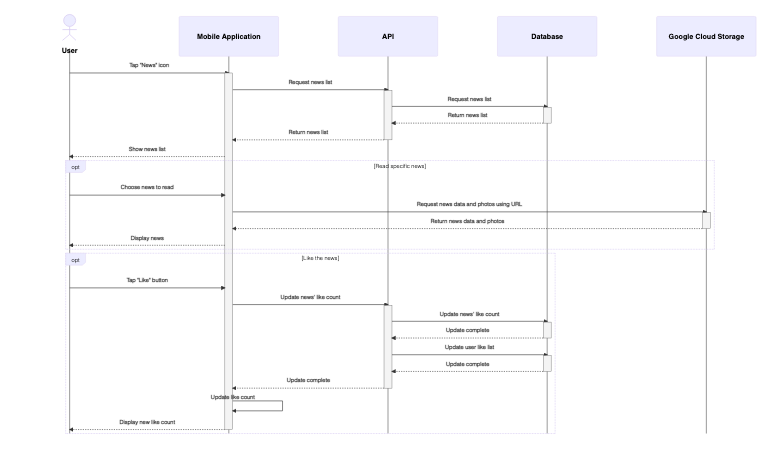
\includegraphics[width=\textwidth]{chapter_3/sequence/News-1.md.png}
    \caption{การทำงานในส่วนข้อมูลข่าวสารของแอปพลิเคชัน}
\end{figure}

\begin{figure}
    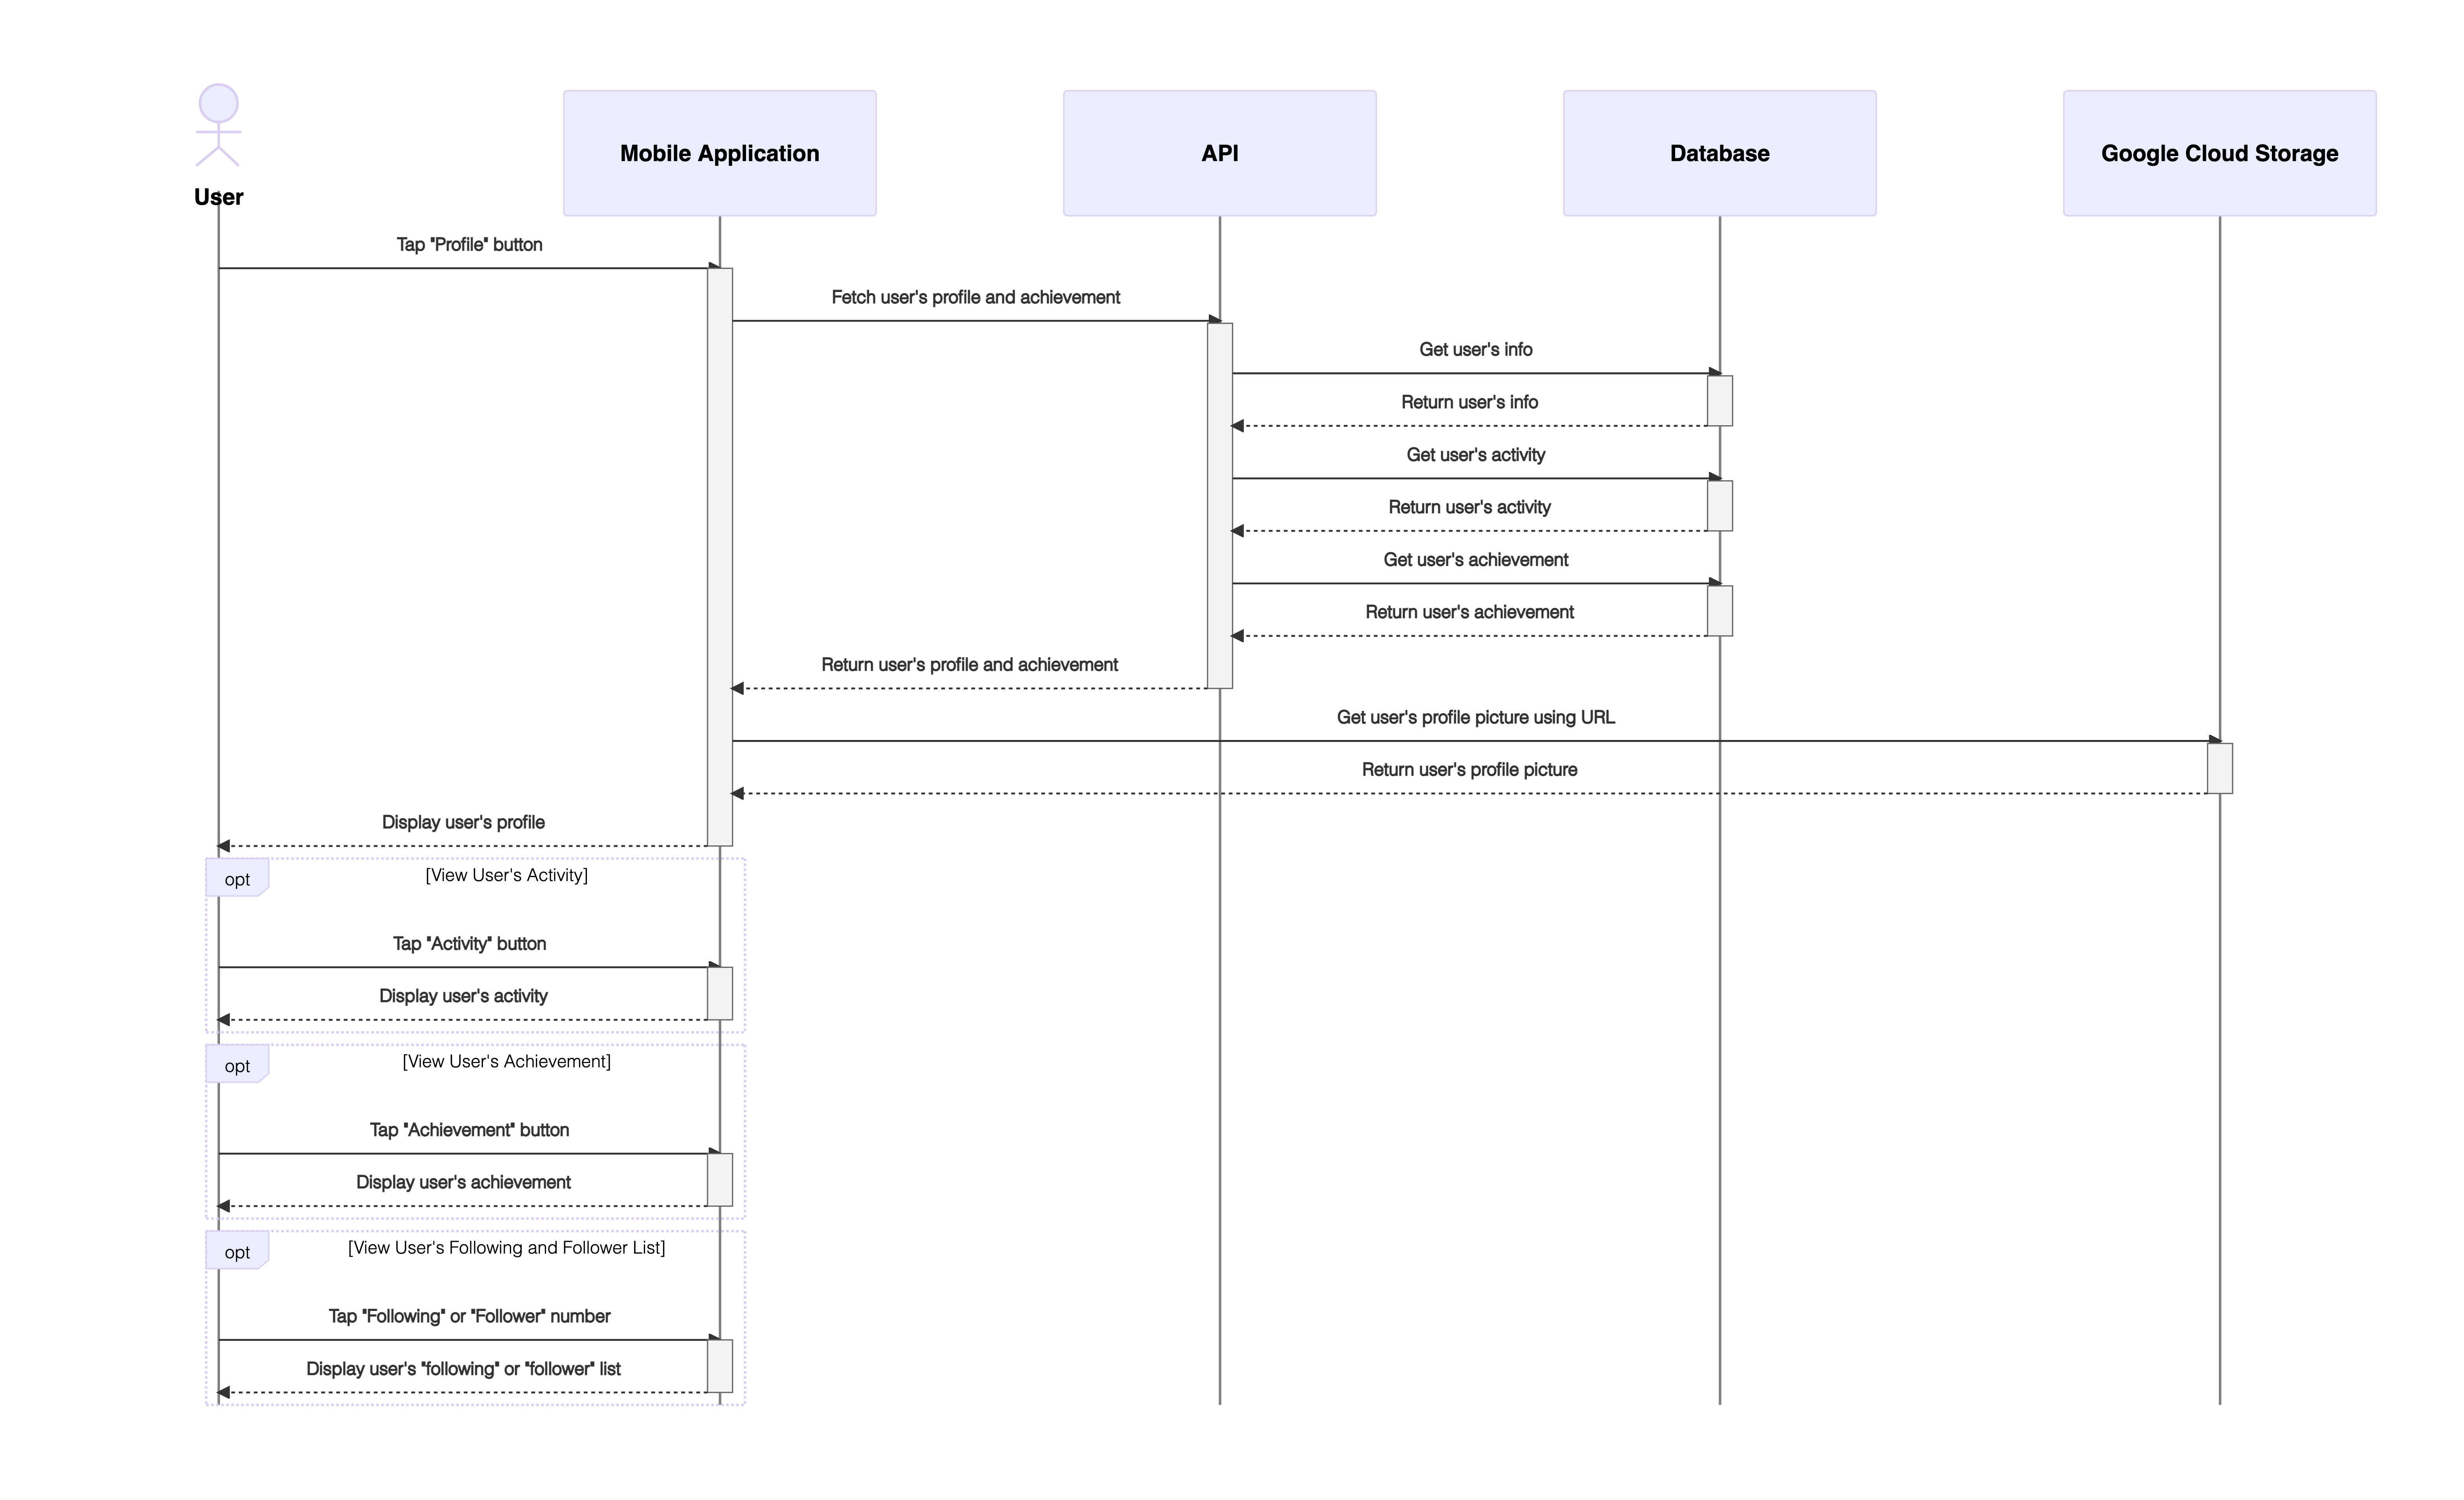
\includegraphics[width=\textwidth]{chapter_3/sequence/User Profile-1.md.png}
    \caption{การทำงานในส่วนข้อมูลของผู้ใช้}
\end{figure}

\begin{figure}
    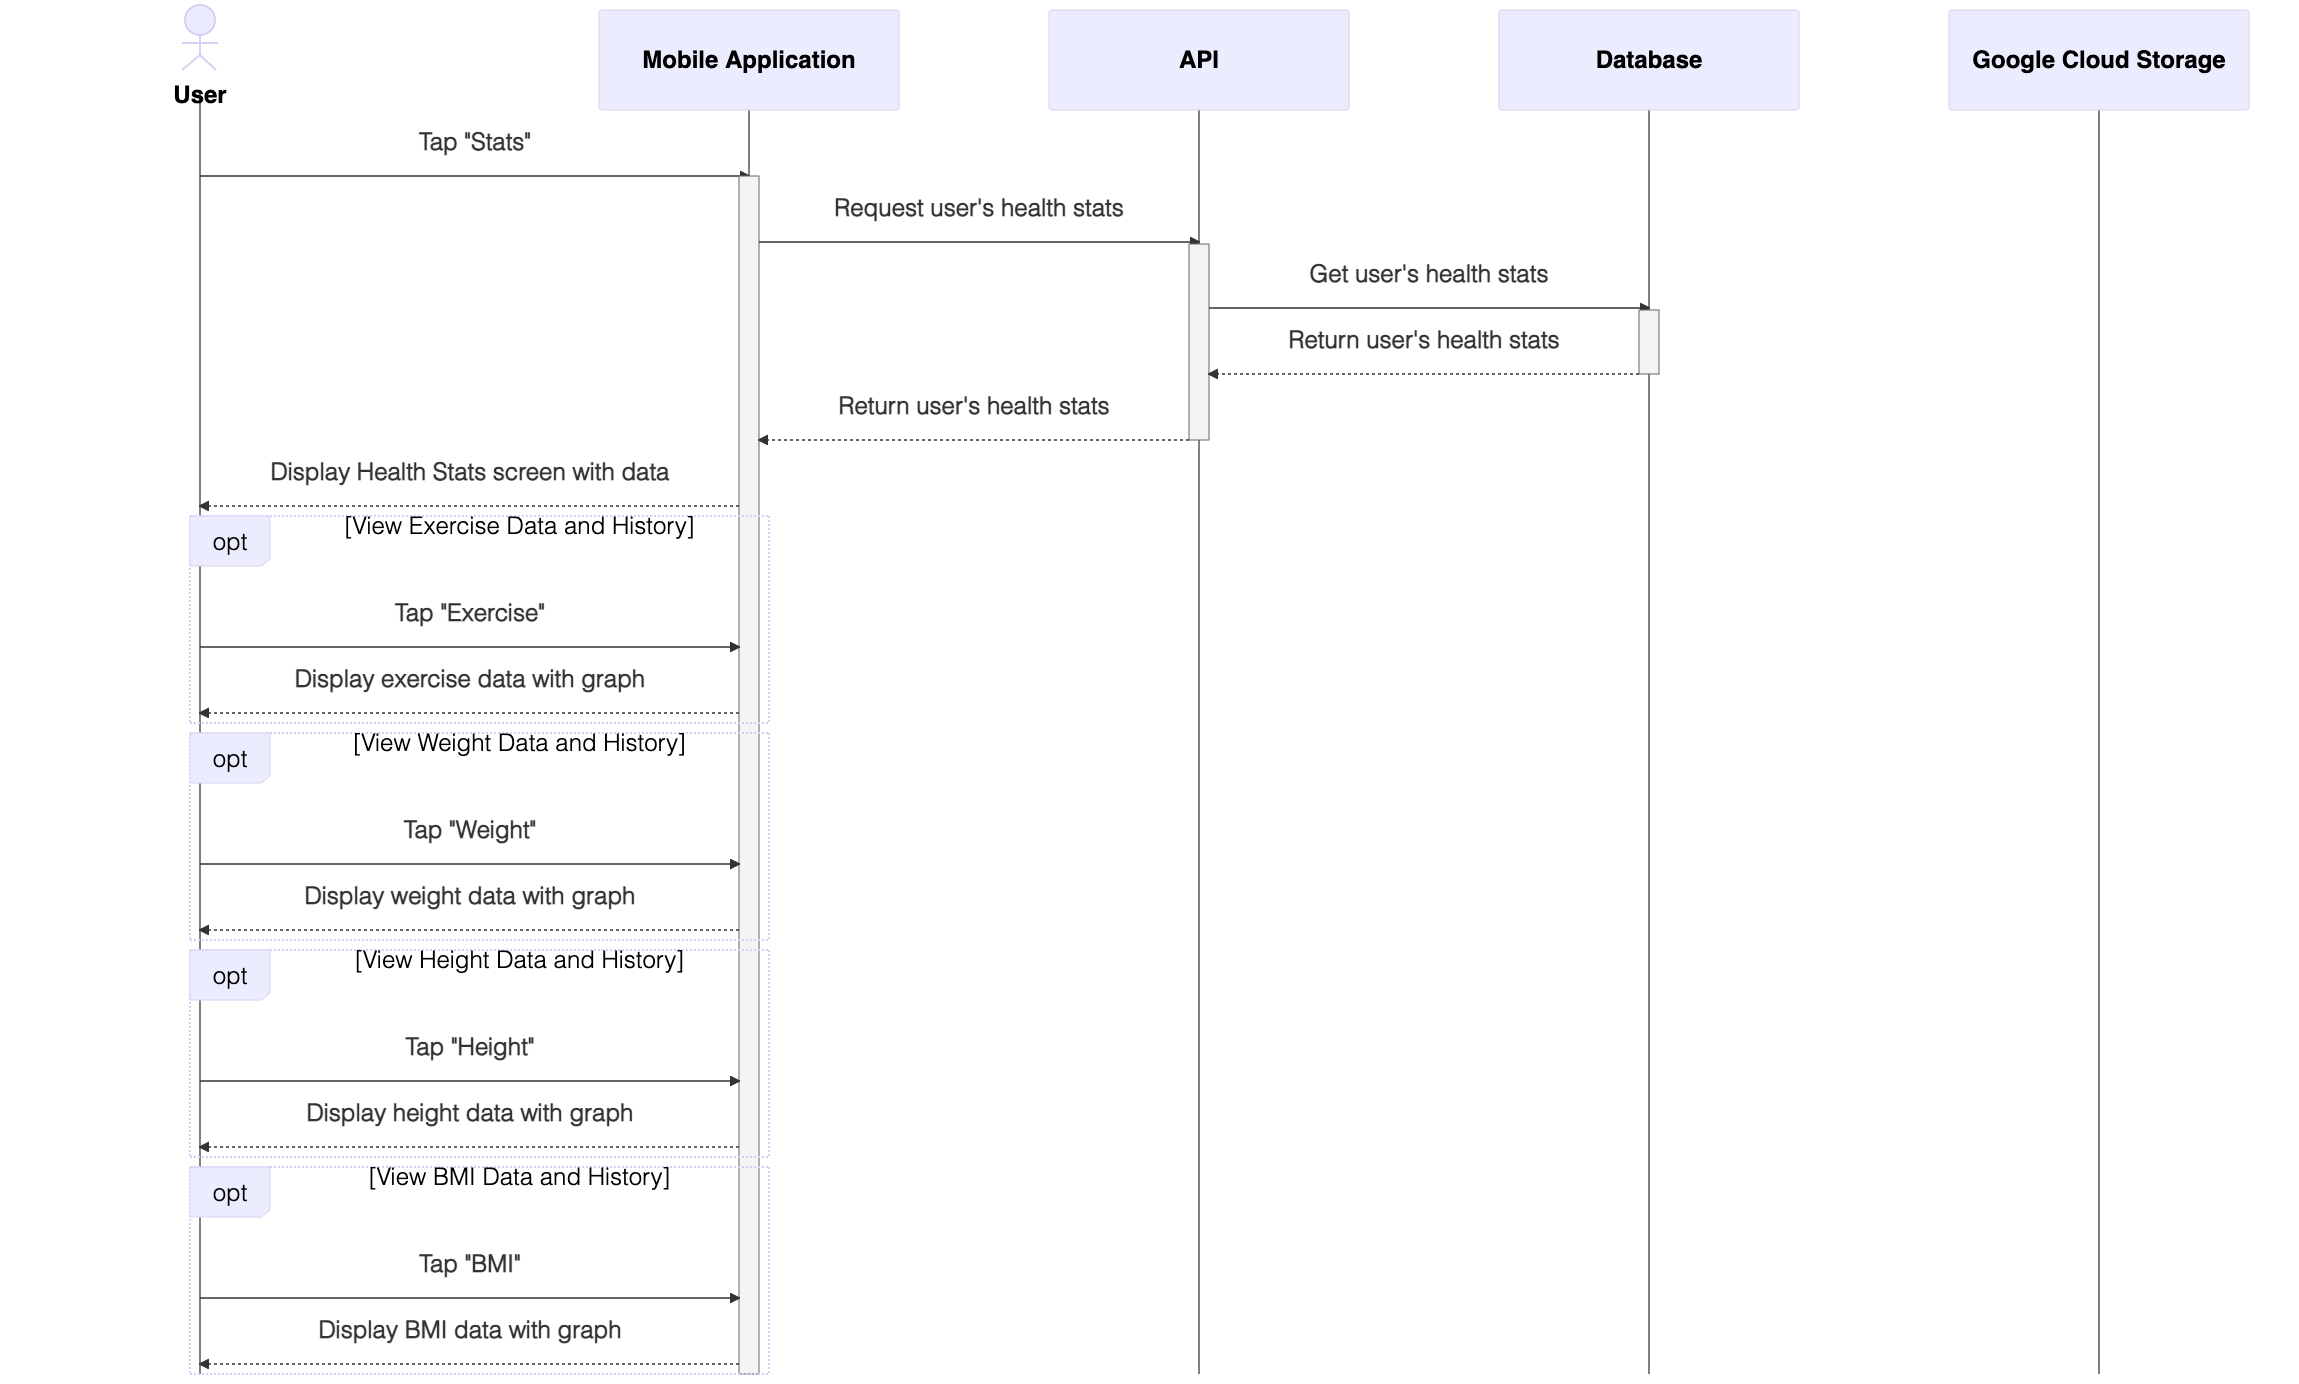
\includegraphics[width=\textwidth]{chapter_3/sequence/View Personal Health Stats-1.md.png}
    \caption{การทำงานในส่วนข้อมูลสุขภาพของผู้ใช้}
\end{figure}

\begin{figure}
    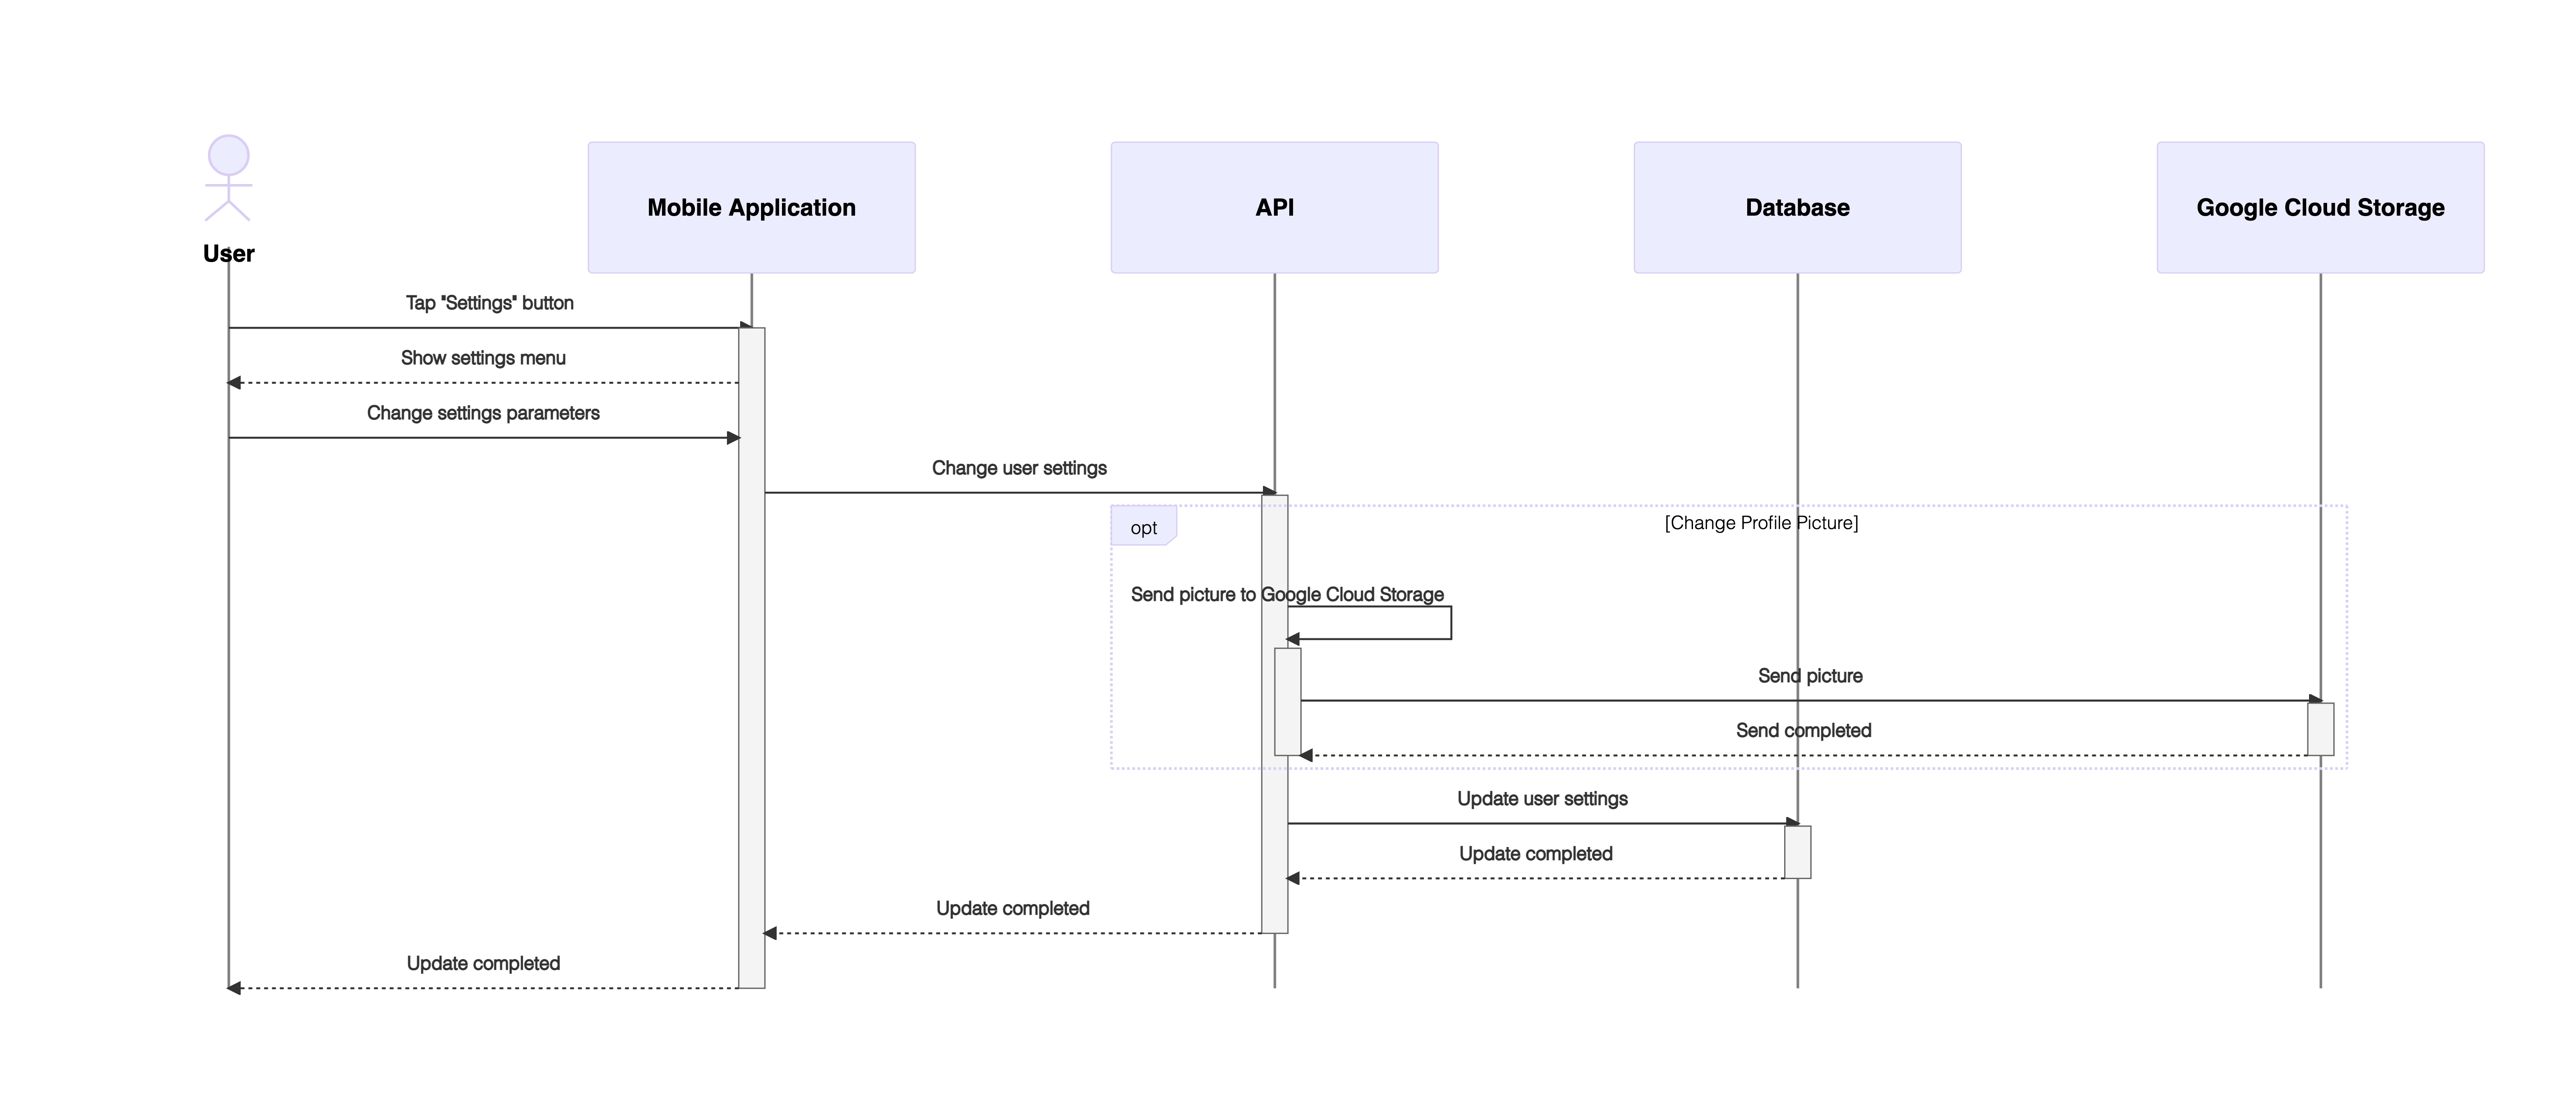
\includegraphics[width=\textwidth]{chapter_3/sequence/User Settings-1.md.png}
    \caption{การทำงานในส่วนการตั้งค่าบัญชีผู้ใช้}
\end{figure}

\clearpage

\section{การออกแบบส่วนติดต่อของผู้ใช้ (User Interface)}

การออกแบบส่วนติดต่อของผู้ใช้ในแอปพลิเคชัน มีดังนี้
\subsection{หน้าเข้าสู่ระบบ}
หน้าเข้าสู่ระบบ จะแสดงขึ้นเมื่อผู้ใช้เข้าสู่แอปพลิเคชัน ผู้ใช้จะต้องกรอก Email และ Password ที่ได้ลงทะเบียนไว้ จากนั้นจึงกด Sign In เพื่อเข้าสู่ระบบ
\begin{figure}
    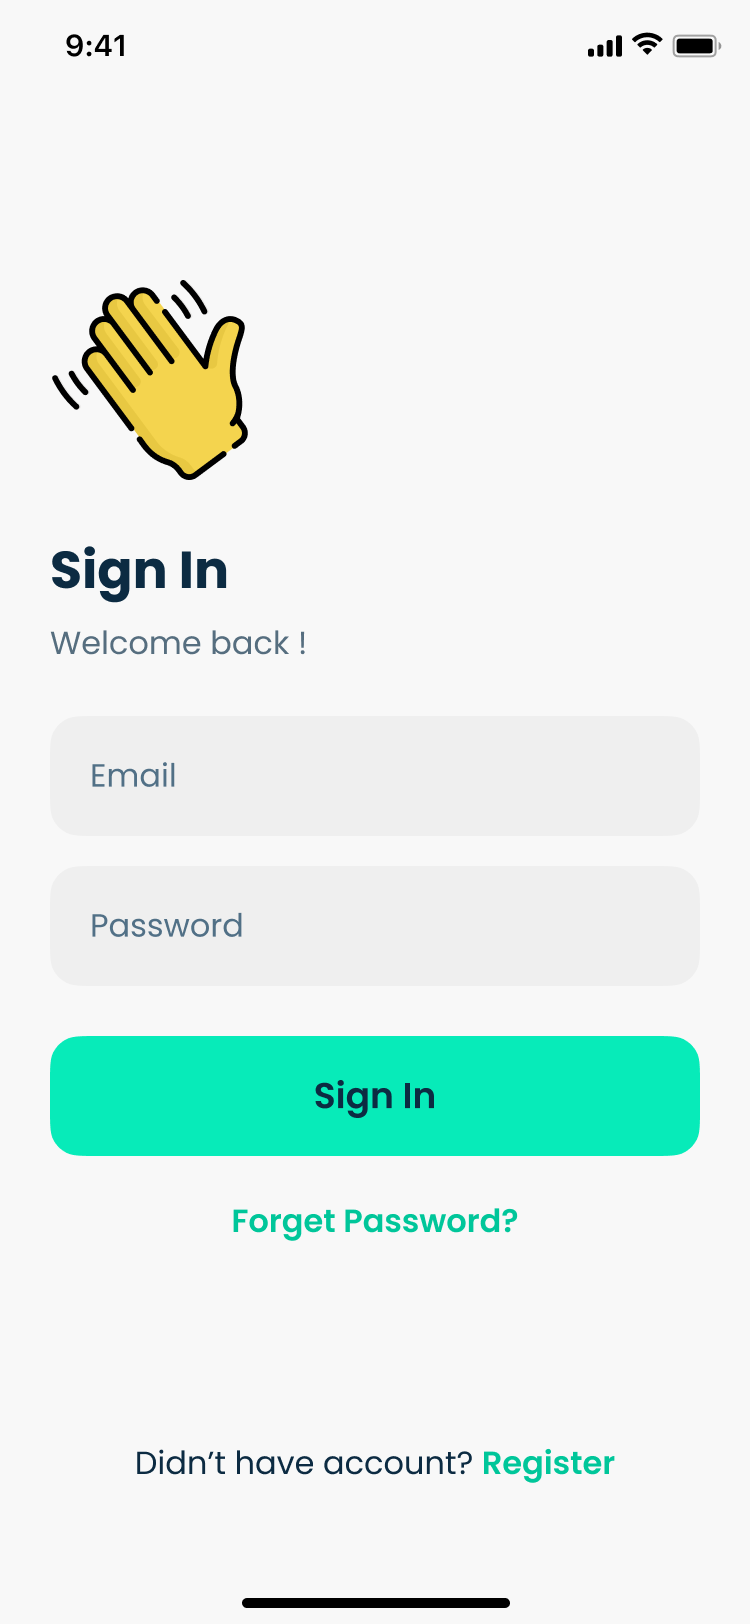
\includegraphics[height=10cm]{chapter_3/ui/Sign In.png}
    \caption{หน้าเข้าสู่ระบบ}
\end{figure}

\subsection{หน้าลงทะเบียน}
หน้าลงทะเบียน จะให้ผู้ใช้กรอกข้อมูลต่าง ๆ ดังนี้
\begin{enumerate}
    \item Email ที่จะใช้ลงทะเบียน
    \item Password ของบัญชี
\end{enumerate}
\begin{figure}
    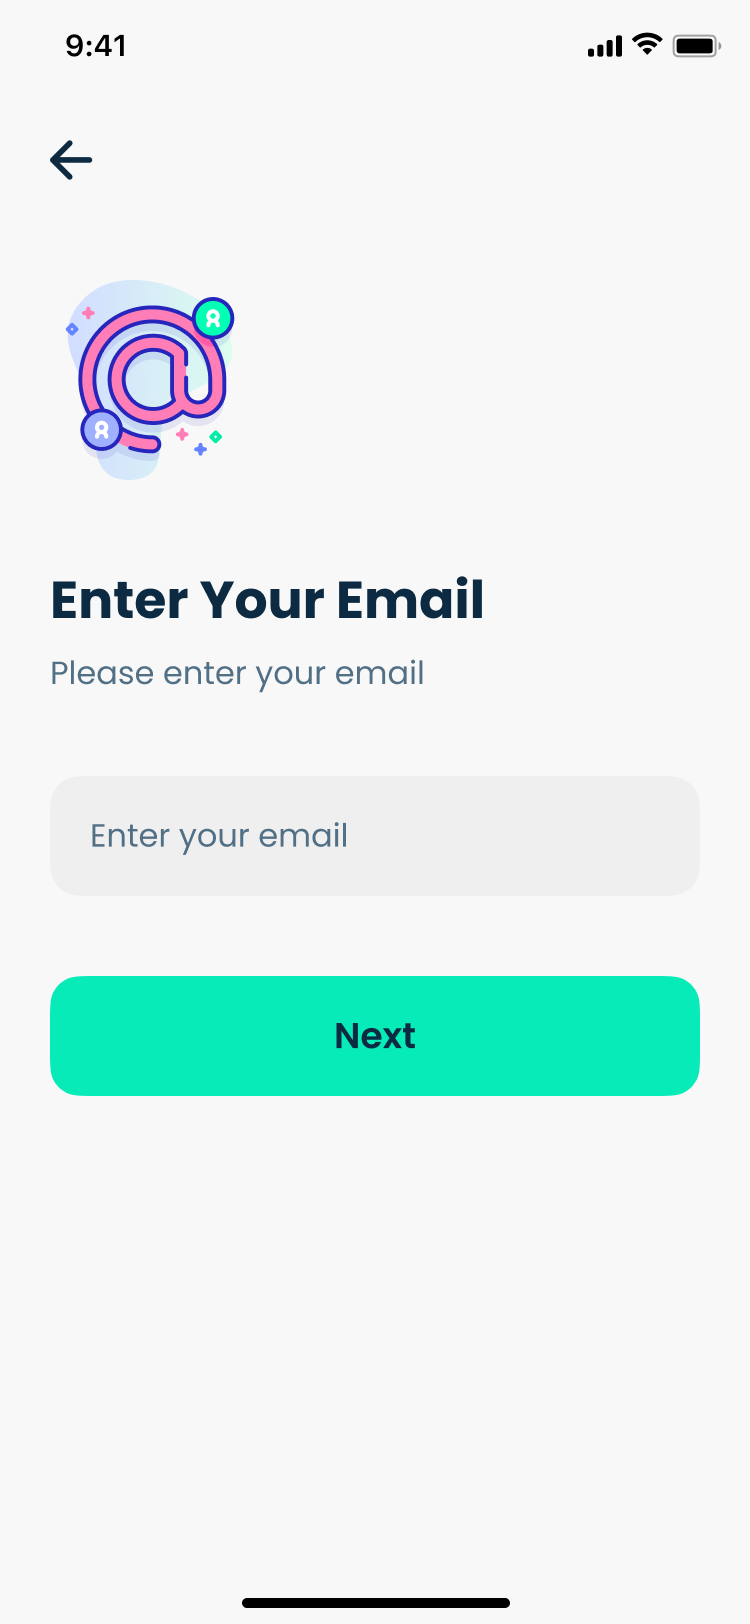
\includegraphics[height=10cm]{chapter_3/ui/Register/Email.png}
    \caption{หน้าการกรอก Email ที่จะใช้ลงทะเบียน}
\end{figure}
\begin{figure}
    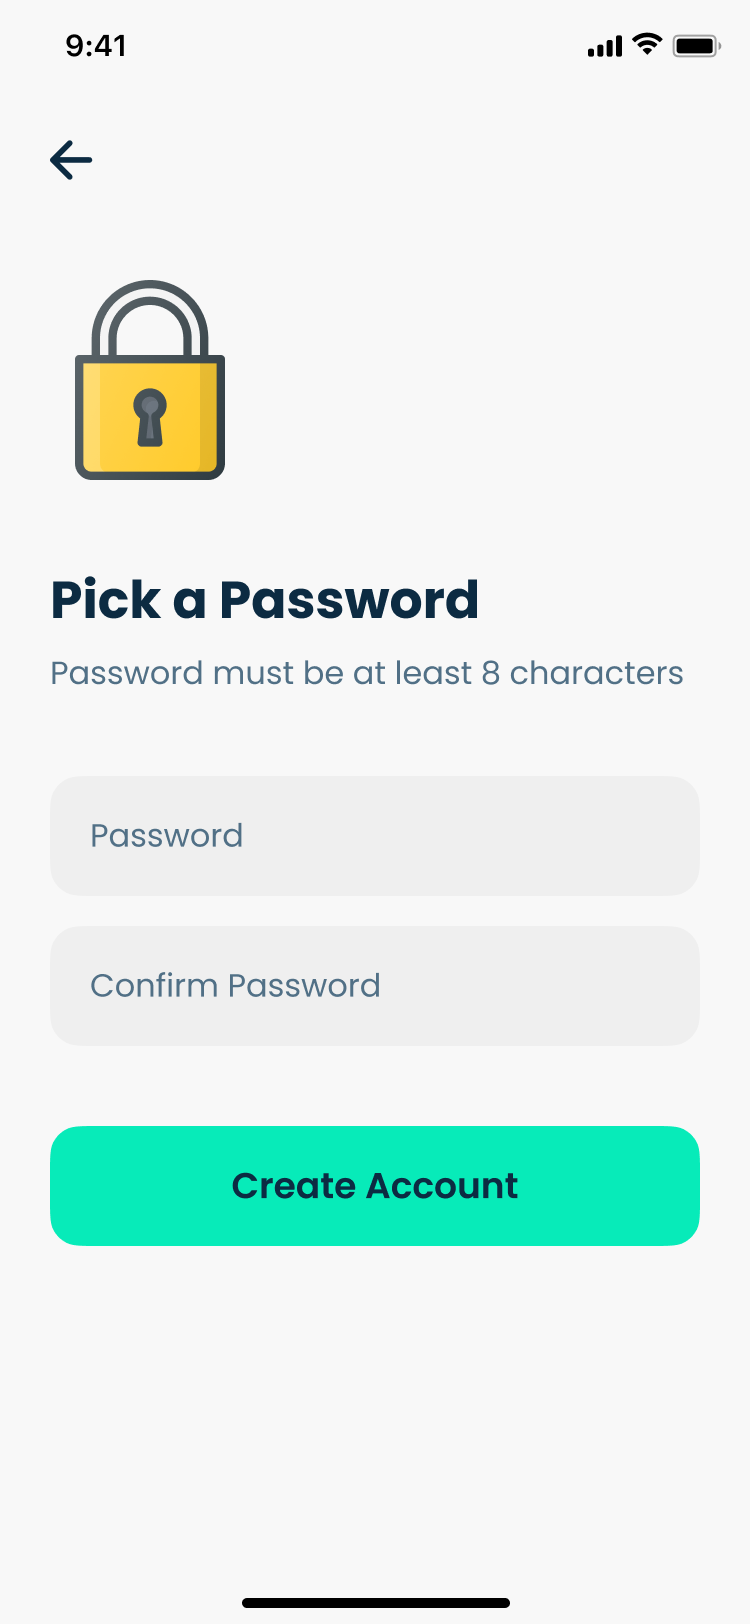
\includegraphics[height=10cm]{chapter_3/ui/Register/Password.png}
    \caption{หน้าการกำหนดรหัสผ่าน}
\end{figure}
\begin{figure}
    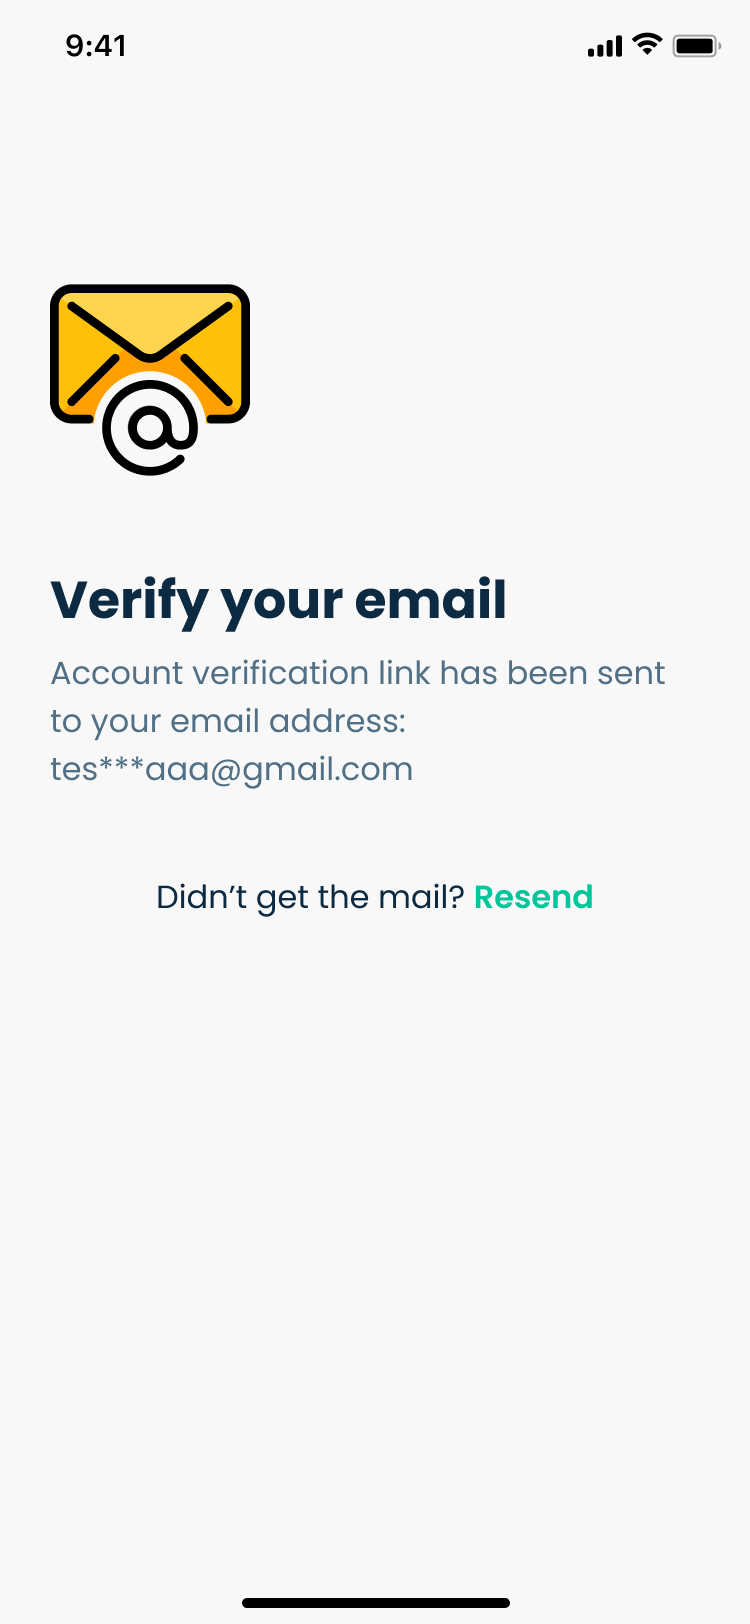
\includegraphics[height=10cm]{chapter_3/ui/Register/Email Verification.png}
    \caption{หน้าการ Verify อีเมล}
\end{figure}
\indent จากนั้น ระบบจะแจ้งให้ผู้ใช้ยืนยัน Email ที่ได้กรอกไว้ ซึ่งจะให้ผู้ใช้ตรวจสอบ Email ที่ระบบได้ส่งไป เมื่อผู้ใช้ยืนยันตัวตนเรียบร้อยแล้ว 
แอปพลิเคชันจะให้ผู้ใช้กรอกข้อมูล ดังนี้
\begin{enumerate}
    \item Display Name สำหรับบัญชีผู้ใช้ ซึ่งจะใช้ในการให้ผู้อื่นสามารถค้นหาบัญชีได้
    \item Profile Picture ให้ผู้ใช้อัปโหลดรูปโปรไฟล์ของตัวเอง ซึ่งผู้ใช้สามารถข้ามขั้นตอนนี้ได้
\end{enumerate}
\begin{figure}
    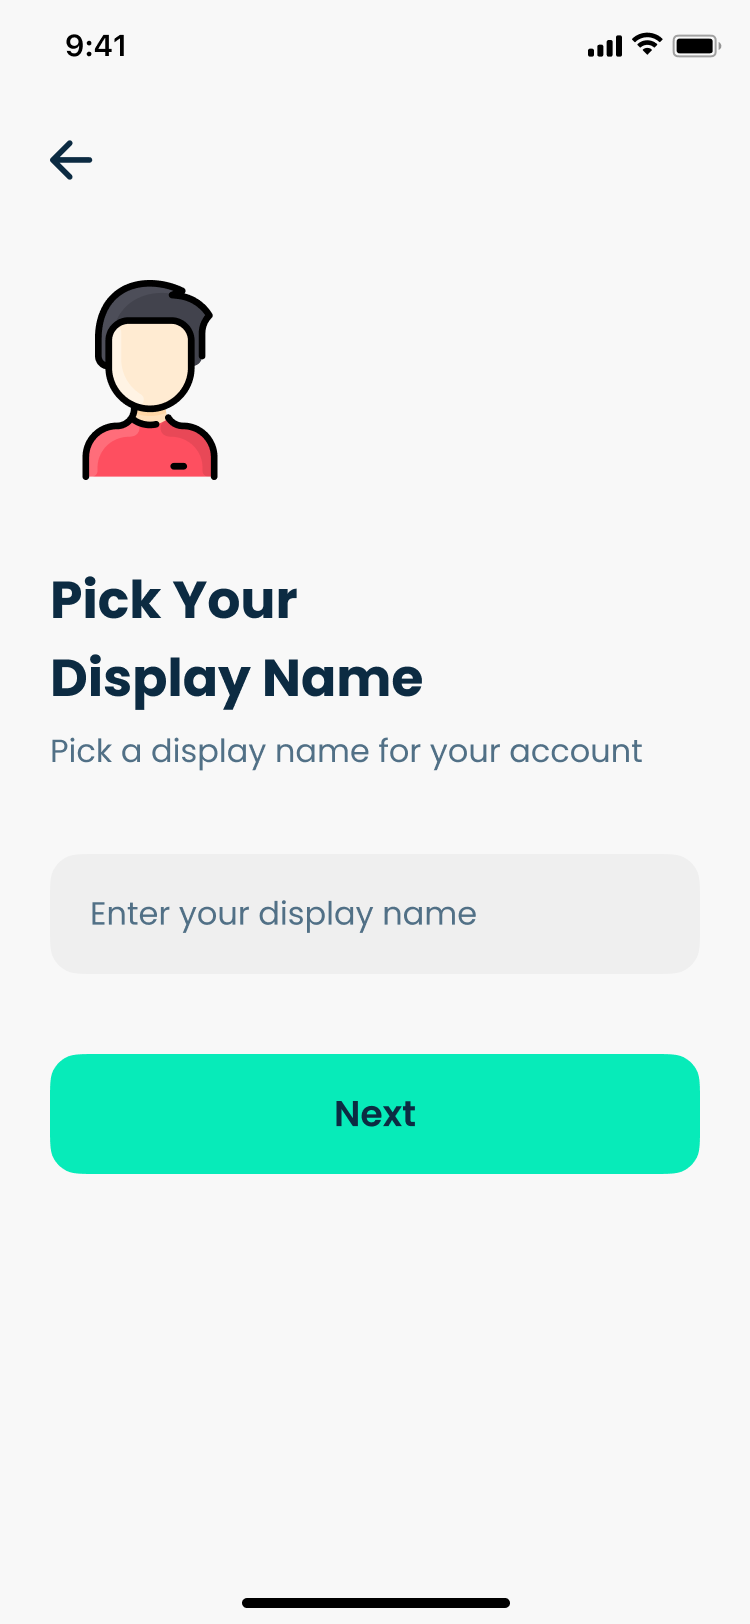
\includegraphics[height=10cm]{chapter_3/ui/Register/Display Name.png}
    \caption{หน้าการ Verify อีเมล}
\end{figure}
\begin{figure}
    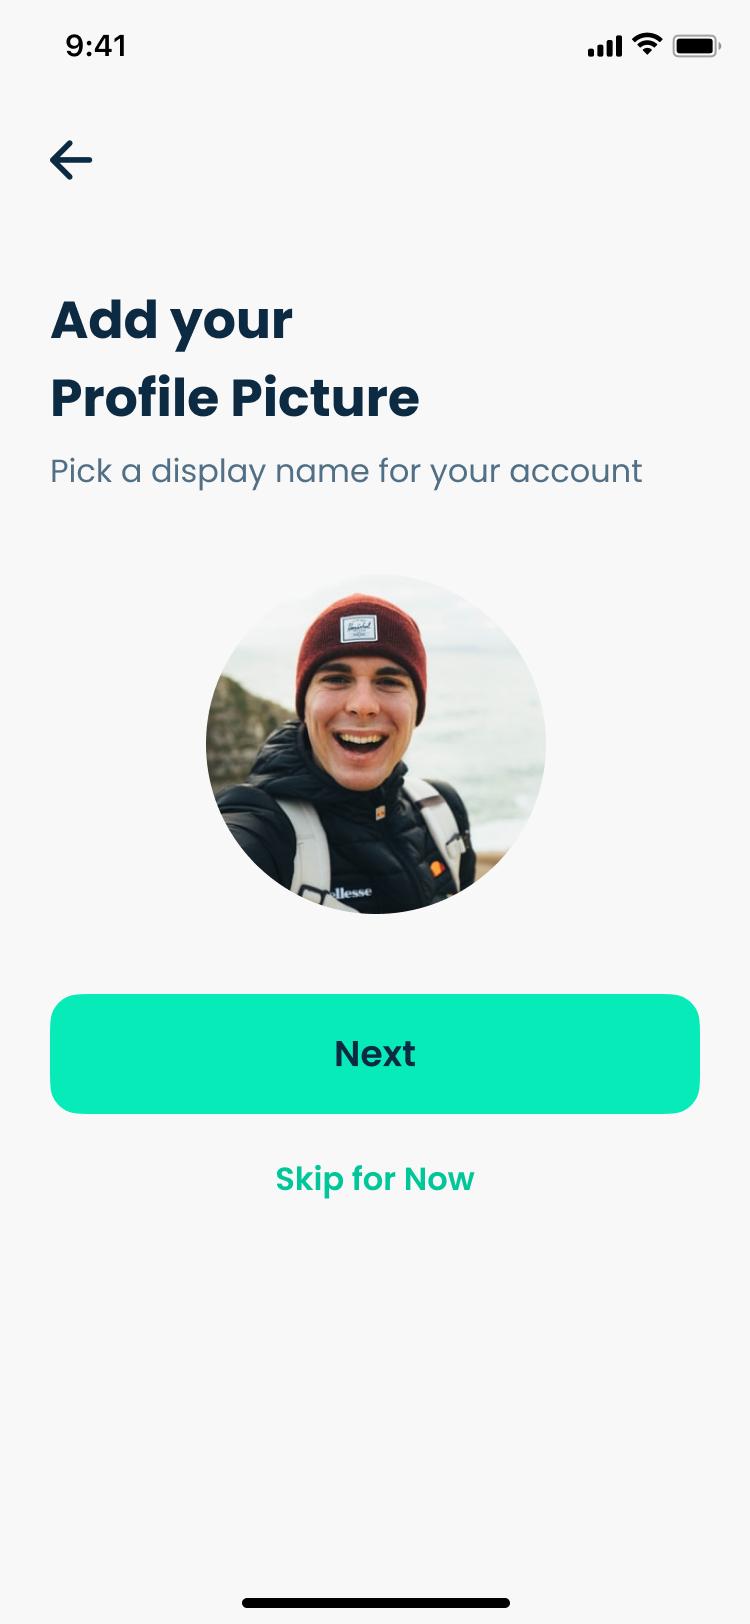
\includegraphics[height=10cm]{chapter_3/ui/Register/Profile Picture.png}
    \caption{หน้าการ Verify อีเมล}
\end{figure}

\subsection{หน้าหลังจากการลงทะเบียน}
เมื่อผู้ใช้ลงทะเบียนเรียบร้อยแล้ว ระบบจะถามคำถามต่าง ๆ เพื่อให้ระบบทราบถึงความต้องการในการออกกำลังกาย และสามารถแนะนำคอร์สออกกำลังกายได้แม่นยำมากขึ้น ซึ่งระบบจะถามคำถาม ดังนี้
\begin{enumerate}
    \item เพศของผู้ใช้
    \item ปีเกิดของผู้ใช้
    \item น้ำหนักและส่วนสูงของผู้ใช้
    \item ประเภทของการออกกำลังกายที่ชื่นชอบ
    \item ส่วนของร่างกายที่ต้องการหลีกเลี่ยง
\end{enumerate}

\begin{figure}
    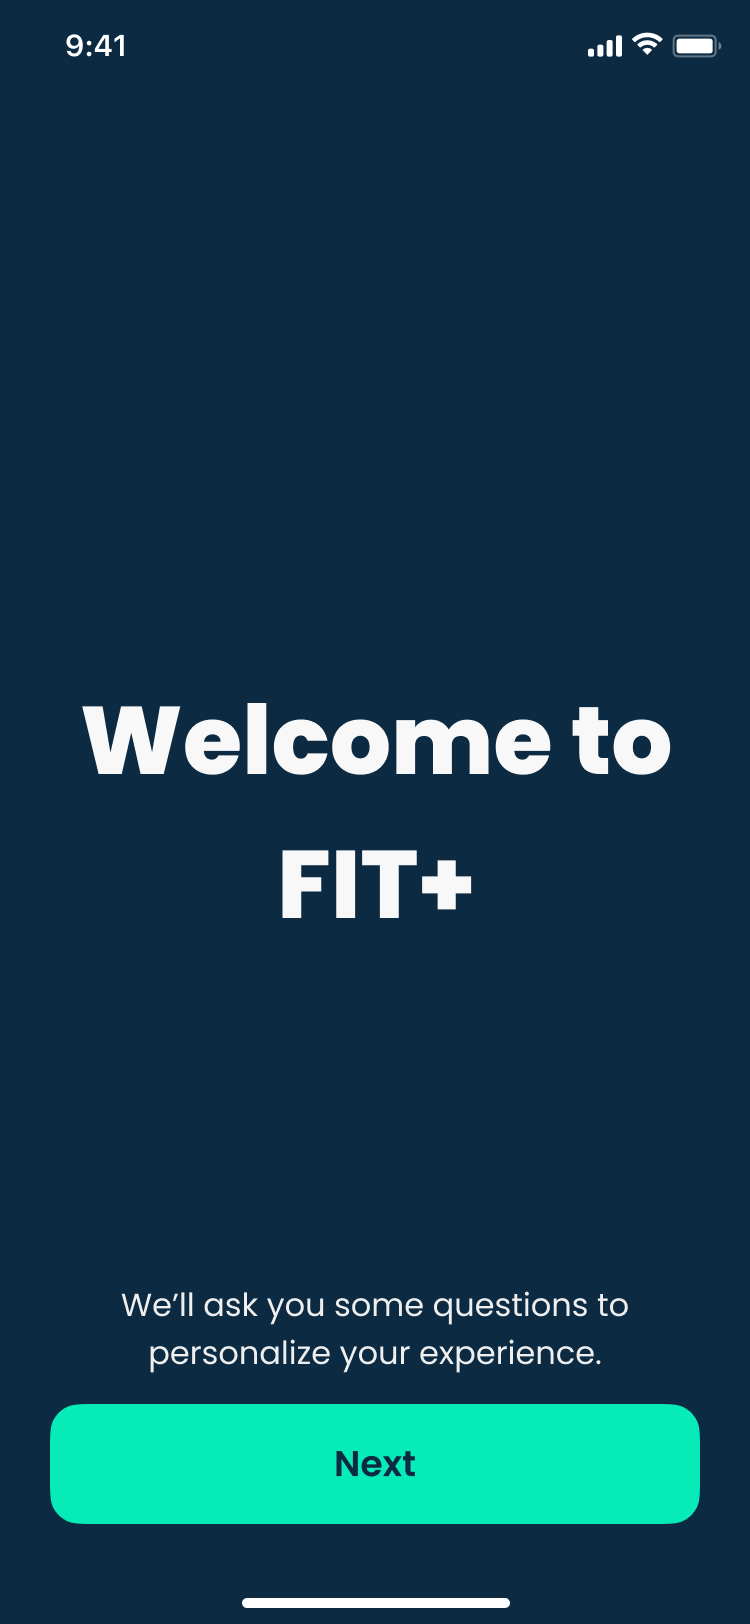
\includegraphics[height=10cm]{chapter_3/ui/New User Setup/000 - Welcome.png}
    \caption{หน้าหลังจากการยืนยันตัวตนเรียบร้อยแล้ว}
\end{figure}
\begin{figure}
    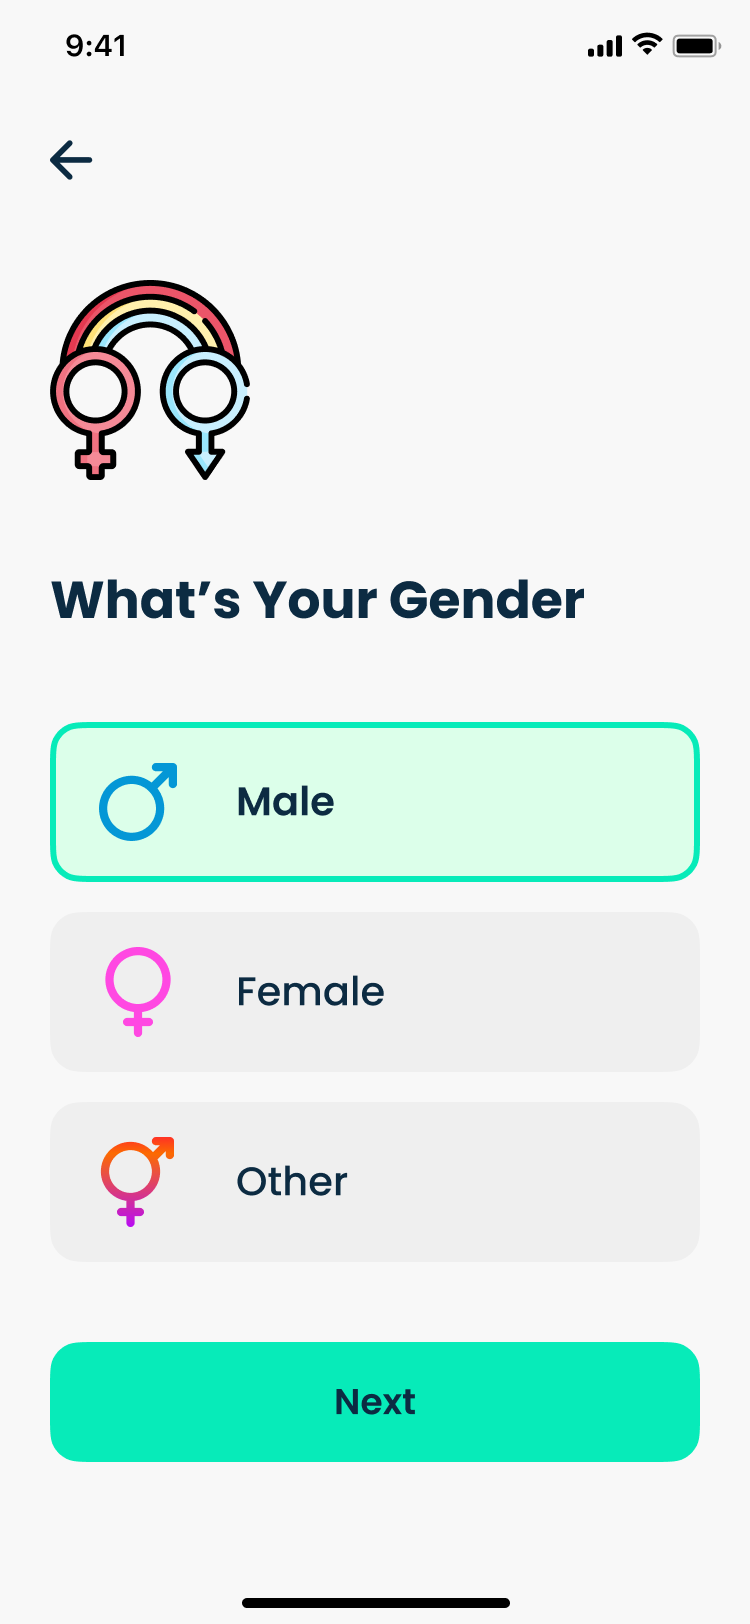
\includegraphics[height=10cm]{chapter_3/ui/New User Setup/001 - Gender.png}
    \caption{หน้าการระบุเพศ}
\end{figure}
\begin{figure}
    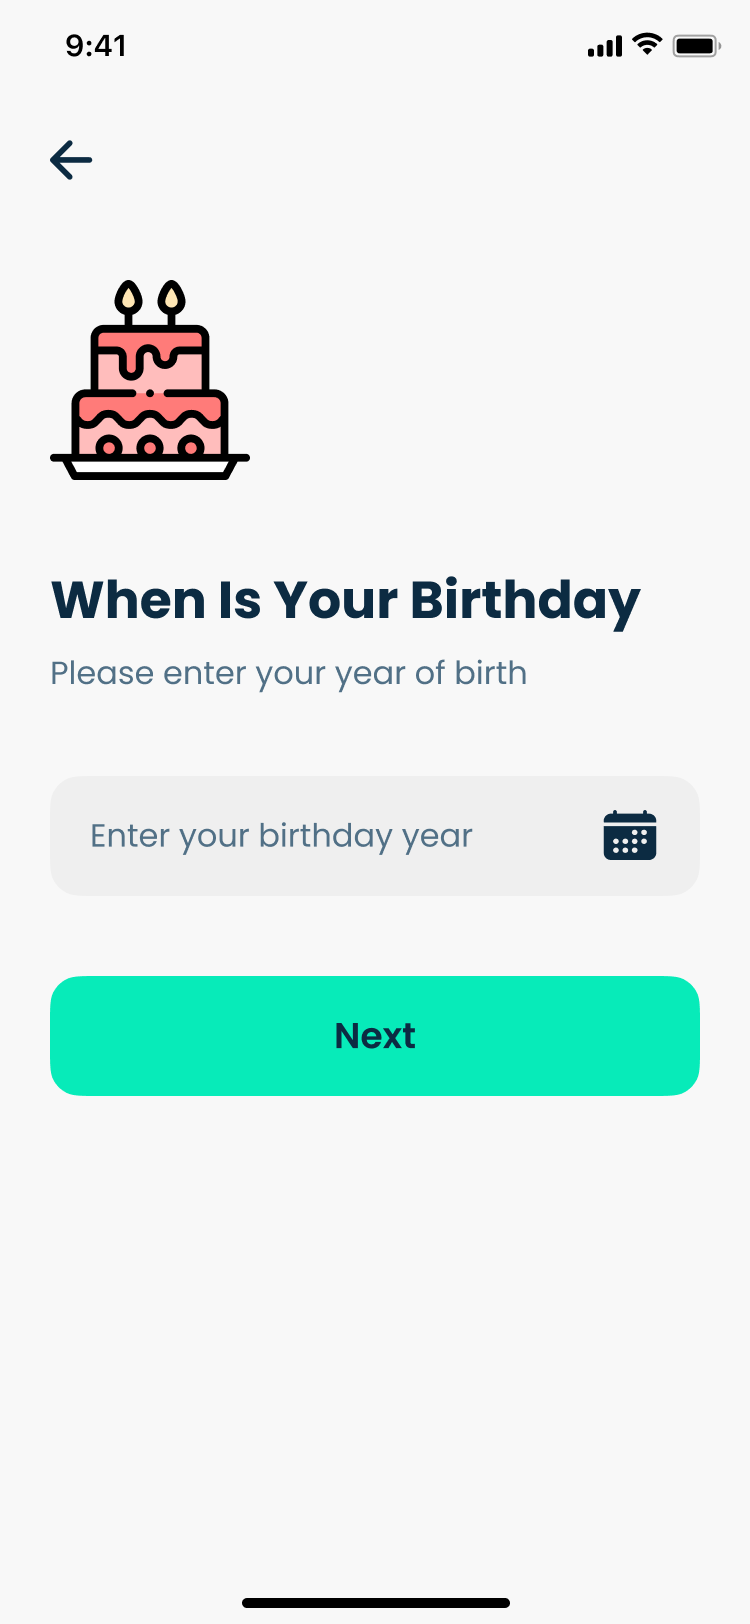
\includegraphics[height=10cm]{chapter_3/ui/New User Setup/002 - Birthday.png}
    \caption{หน้าการกรอกข้อมูลวันเกิด}
\end{figure}
\begin{figure}
    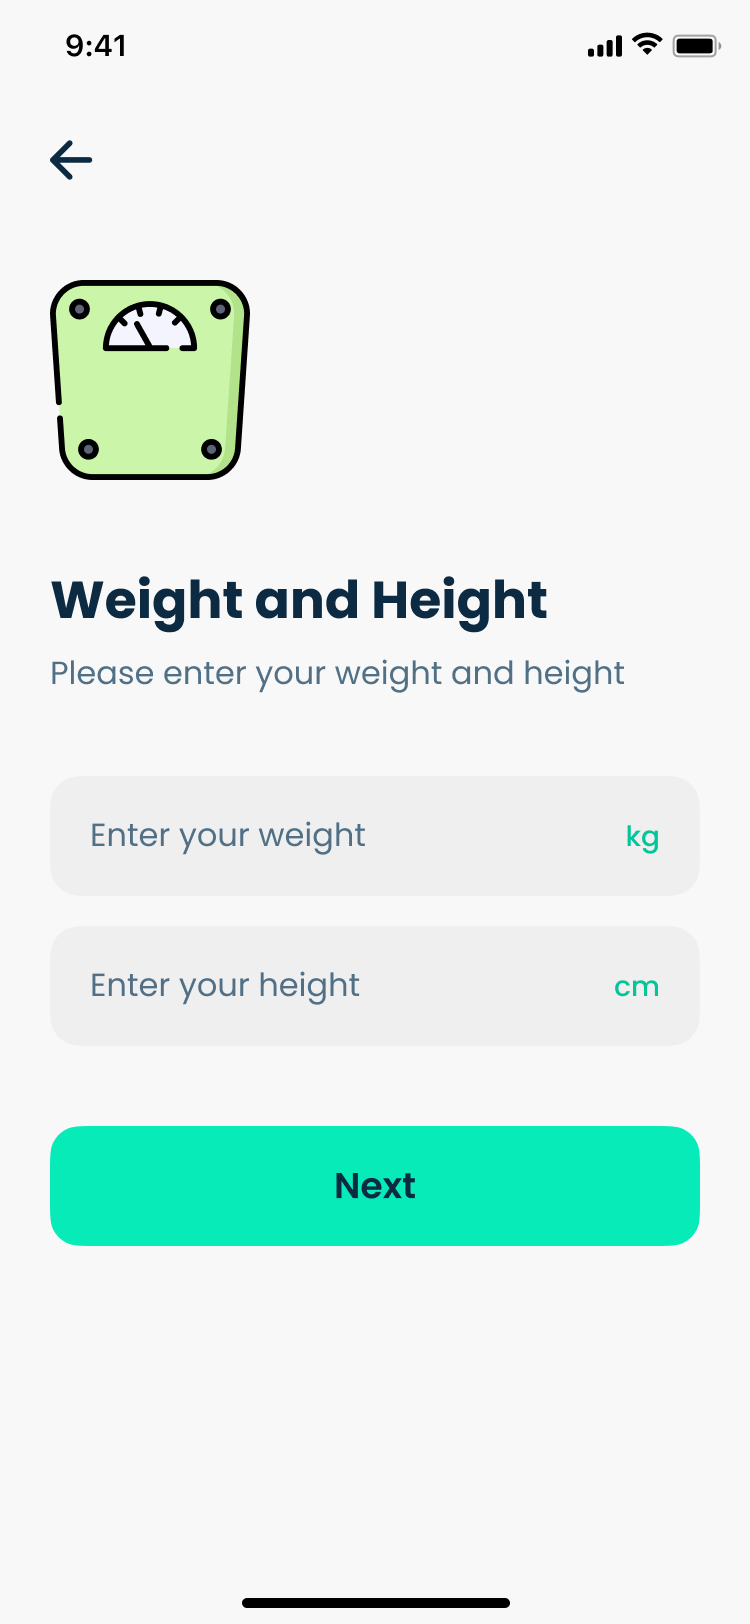
\includegraphics[height=10cm]{chapter_3/ui/New User Setup/003 - Weight and Height.png}
    \caption{หน้าการกรอกข้อมูลน้ำหนักและส่วนสูง}
\end{figure}
\begin{figure}
    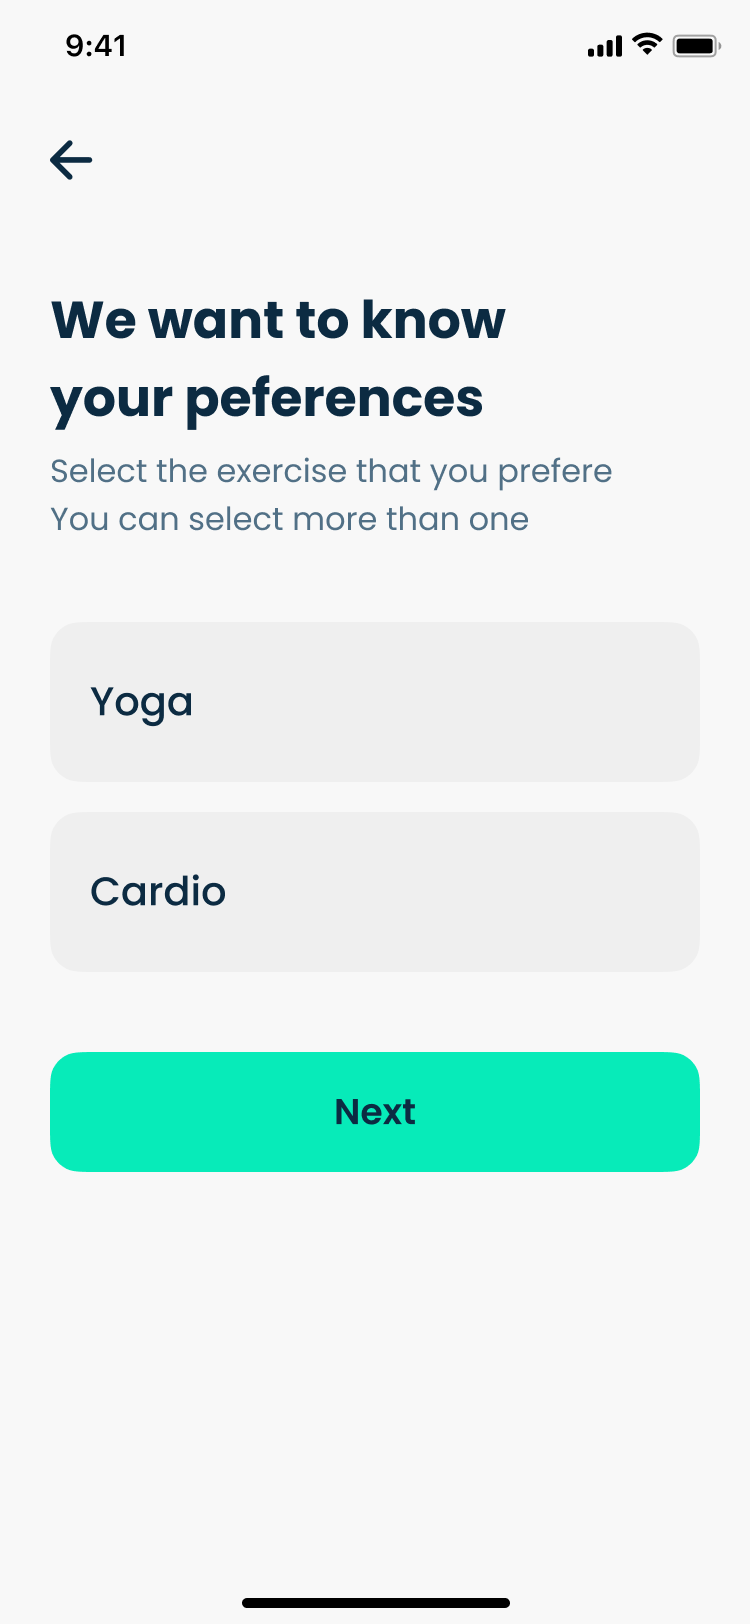
\includegraphics[height=10cm]{chapter_3/ui/New User Setup/004 - Exercise Preferences.png}
    \caption{หน้าการระบุประเภทของการออกกำลังกายที่ชื่นชอบ}
\end{figure}
\begin{figure}
    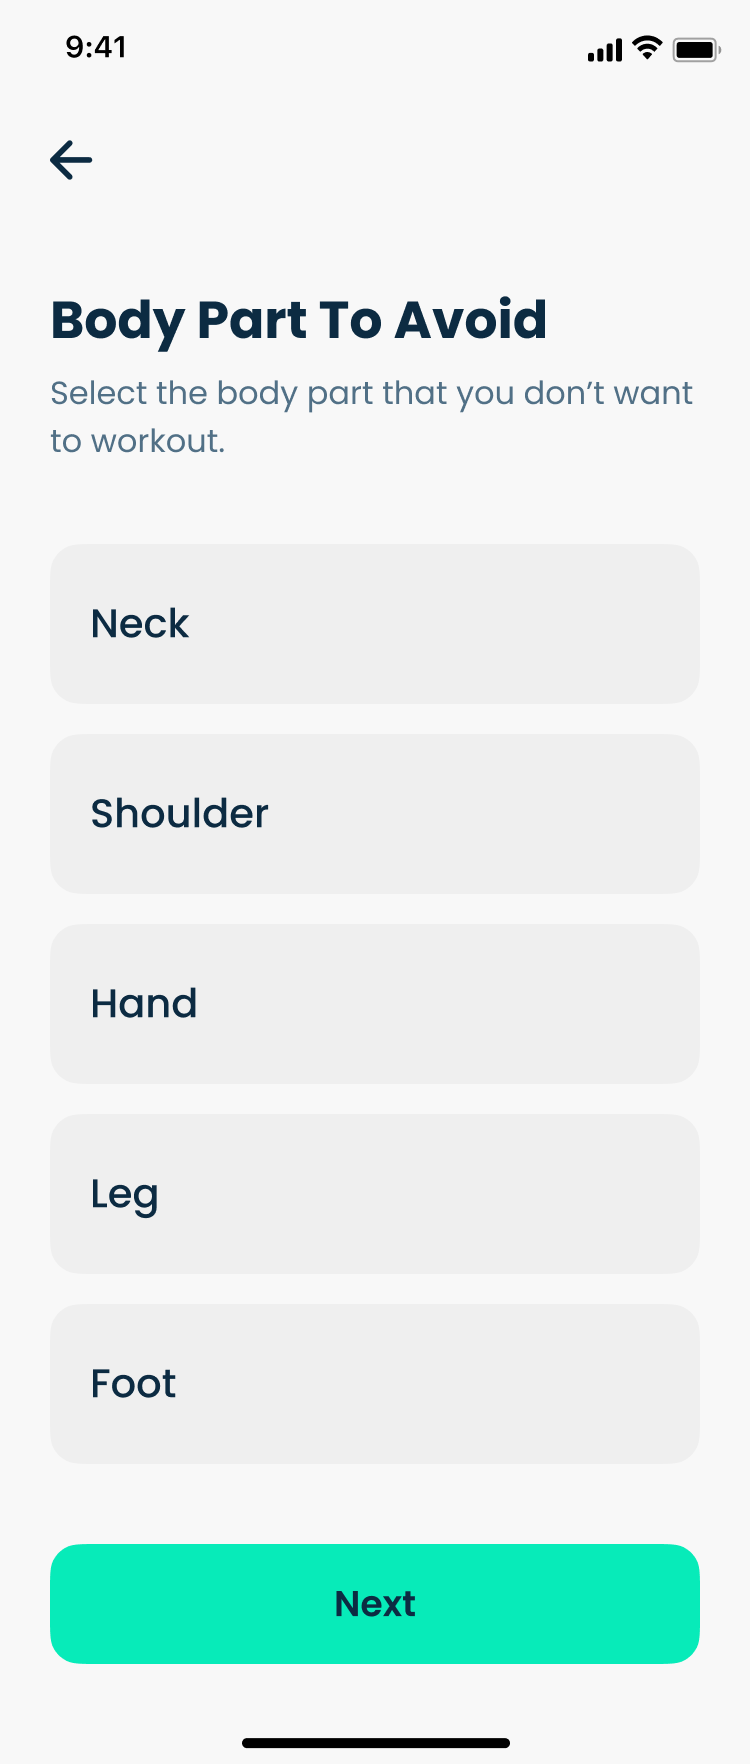
\includegraphics[height=10cm]{chapter_3/ui/New User Setup/005 - Exercise Preferences.png}
    \caption{หน้าการระบุส่วนของร่างกายที่ต้องการหลีกเลี่ยง}
\end{figure}
\begin{figure}
    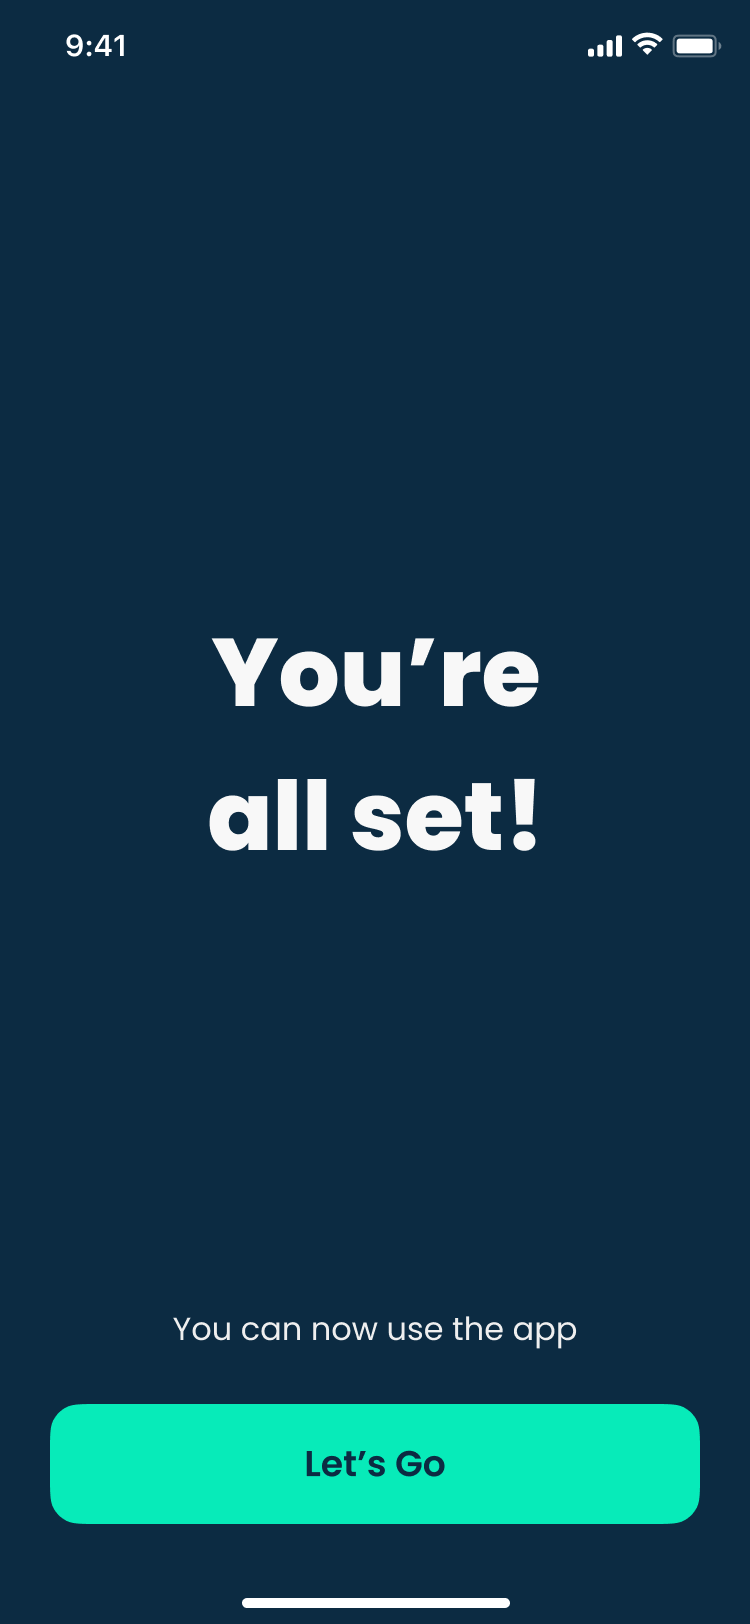
\includegraphics[height=10cm]{chapter_3/ui/New User Setup/006 - Complete.png}
    \caption{หน้าหลังจากการตอบคำถามความต้องการออกกำลังกาย}
\end{figure}

\subsection{หน้าแรกของแอปพลิเคชัน}
หน้าแรกของแอปพลิเคชัน จะแสดงผลคอร์สต่าง ๆ ที่เป็นที่นิยม และเหมาะสมสำหรับผู้ใช้ และแถบ Banner สำหรับการประชาสัมพันธ์คอร์สหรือข่าวสารต่าง ๆ ของทางแอปพลิเคชัน และด้านมุมบนขวาจะมีปุ่มค้นหา โดยจะสามารถค้นหาคอร์ส และบัญชีผู้ใช้ในระบบได้
\begin{figure}
    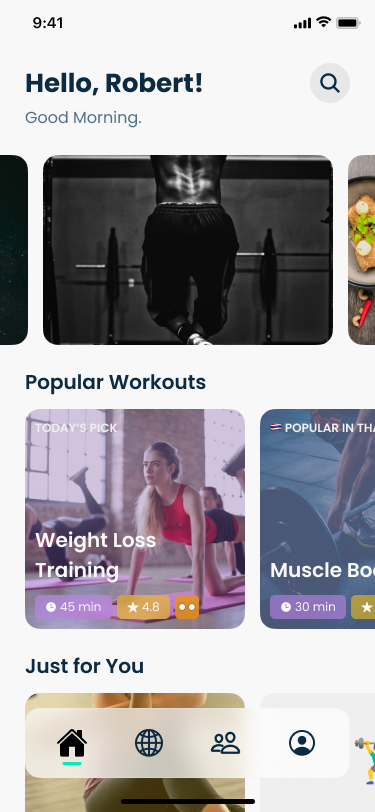
\includegraphics[height=10cm]{chapter_3/ui/Home.png}
    \caption{หน้าแรกของแอปพลิเคชัน}
\end{figure}

\subsection{หน้ากิจกรรมของผู้ใช้}
หน้ากิจกรรมของผู้ใช้ จะแสดงความเคลื่อนไหวต่าง ๆ ของบุคคลที่ผู้ใช้ได้ติดตามไว้ ผู้ใช้สามารถกด Reaction และ Comment กิจกรรมของบุคคลนั้น ๆ ได้ ด้านมุมขววาบนจะเป็นปุ่มตารางคะแนน Leaderboard ซึ่งจะสามารถให้ผู้ใช้ดูคะแนนสะสมของบัญชีที่ผู้ใช้ติดตามได้ และสามารถเปรียบเทียบคะแนนกับผู้ใช้ทั้งหมดในระบบได้
\begin{figure}
    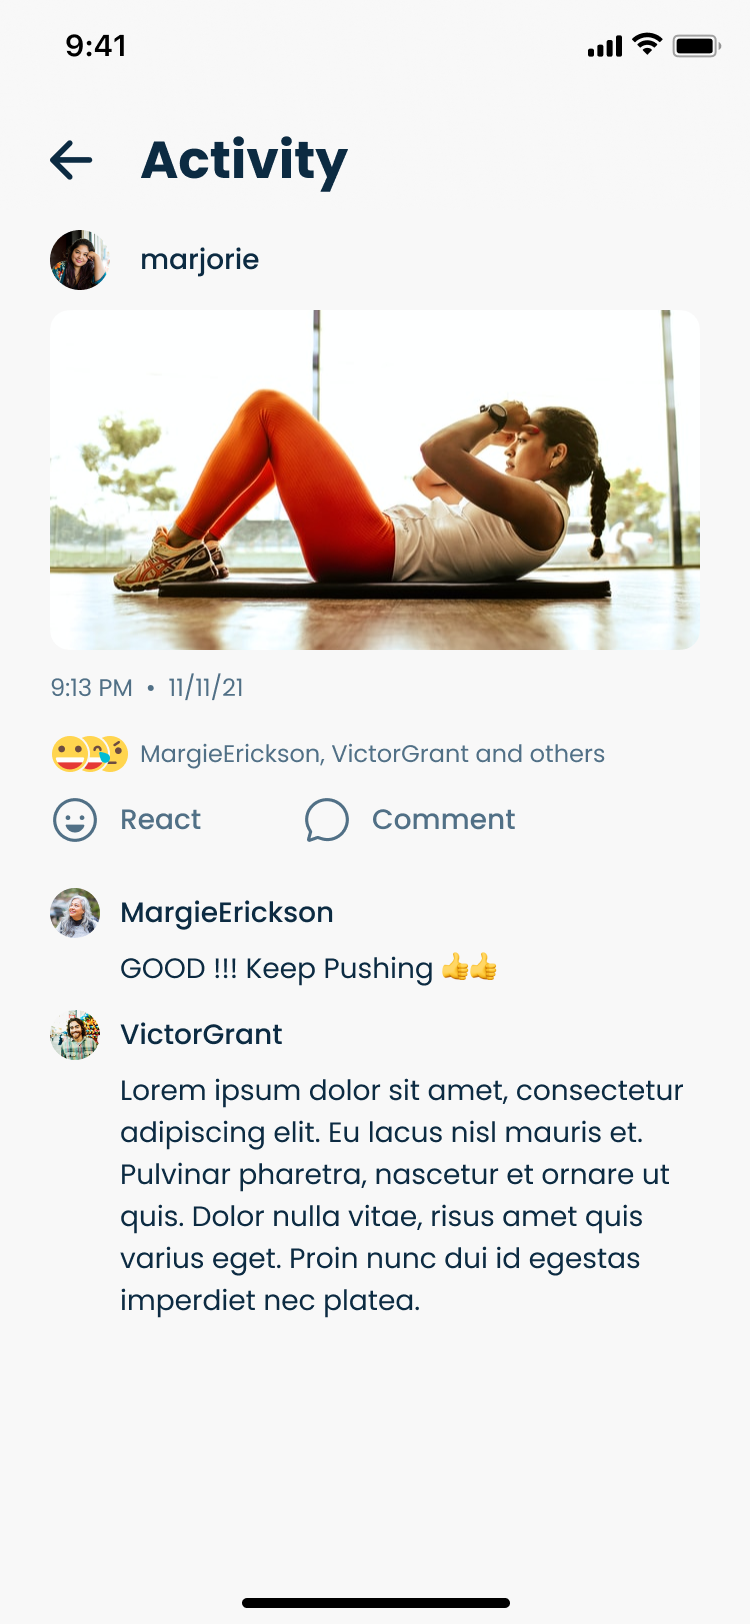
\includegraphics[height=10cm]{chapter_3/ui/Social/Activity.png}
    \caption{หน้ากิจกรรมของผู้ใช้}
\end{figure}
\begin{figure}
    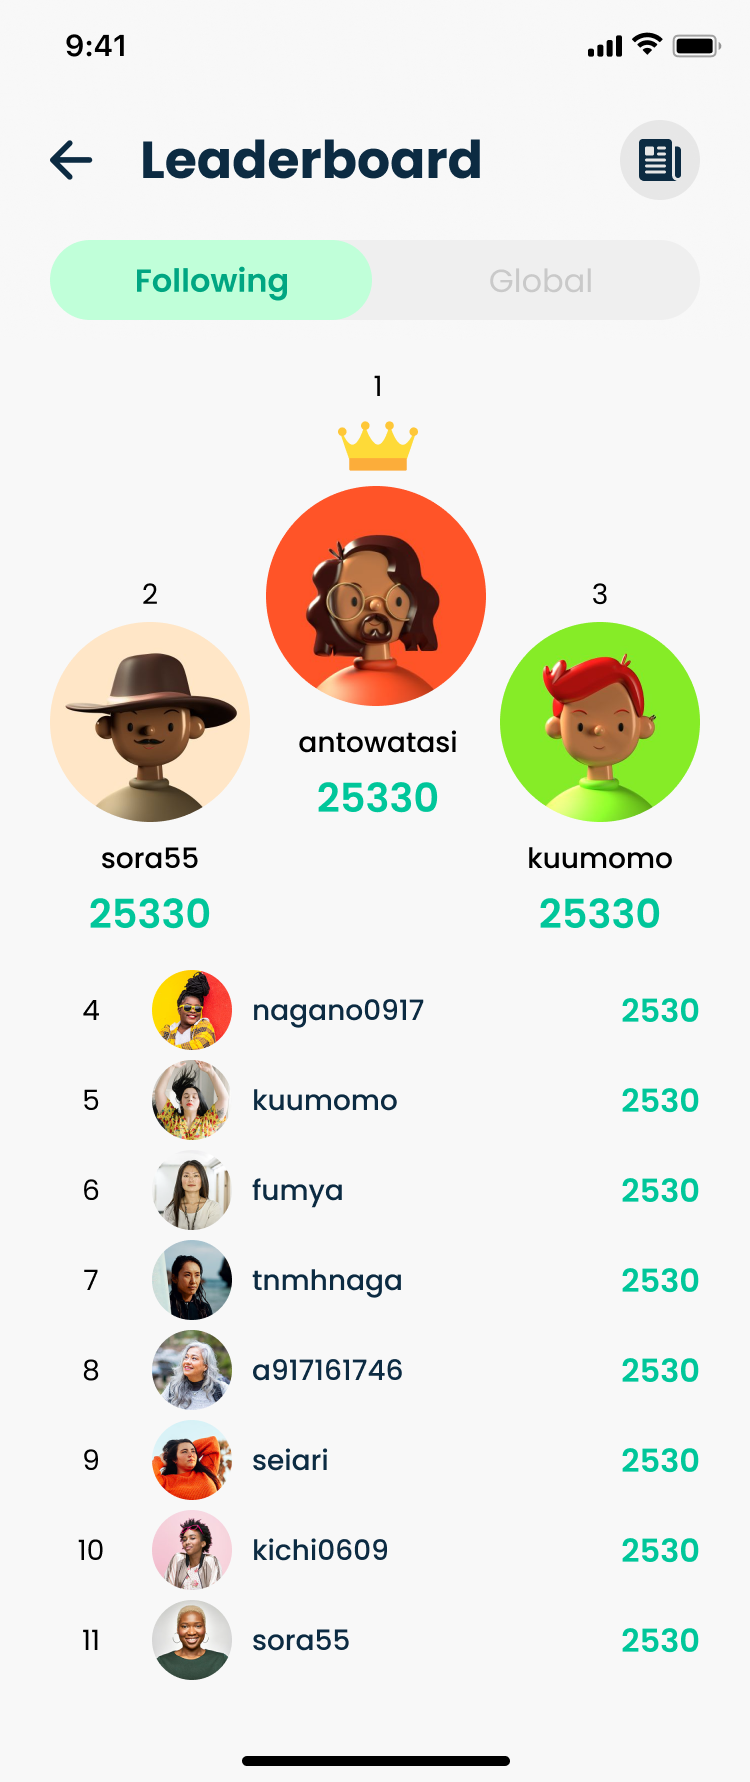
\includegraphics[height=10cm]{chapter_3/ui/Social/Leaderboard.png}
    \caption{หน้าตารางคะแนน Leaderboard}
\end{figure}

\subsection{หน้าข่าวสาร}
หน้าข่าวสารของแอปพลิเคชัน ซึ่งจะให้ผู้ใช้สามารถดูข่าวสารด้านการออกกำลังกายได้ และสามารถกดปุ่มชื่นชอบบทความได้
\begin{figure}
    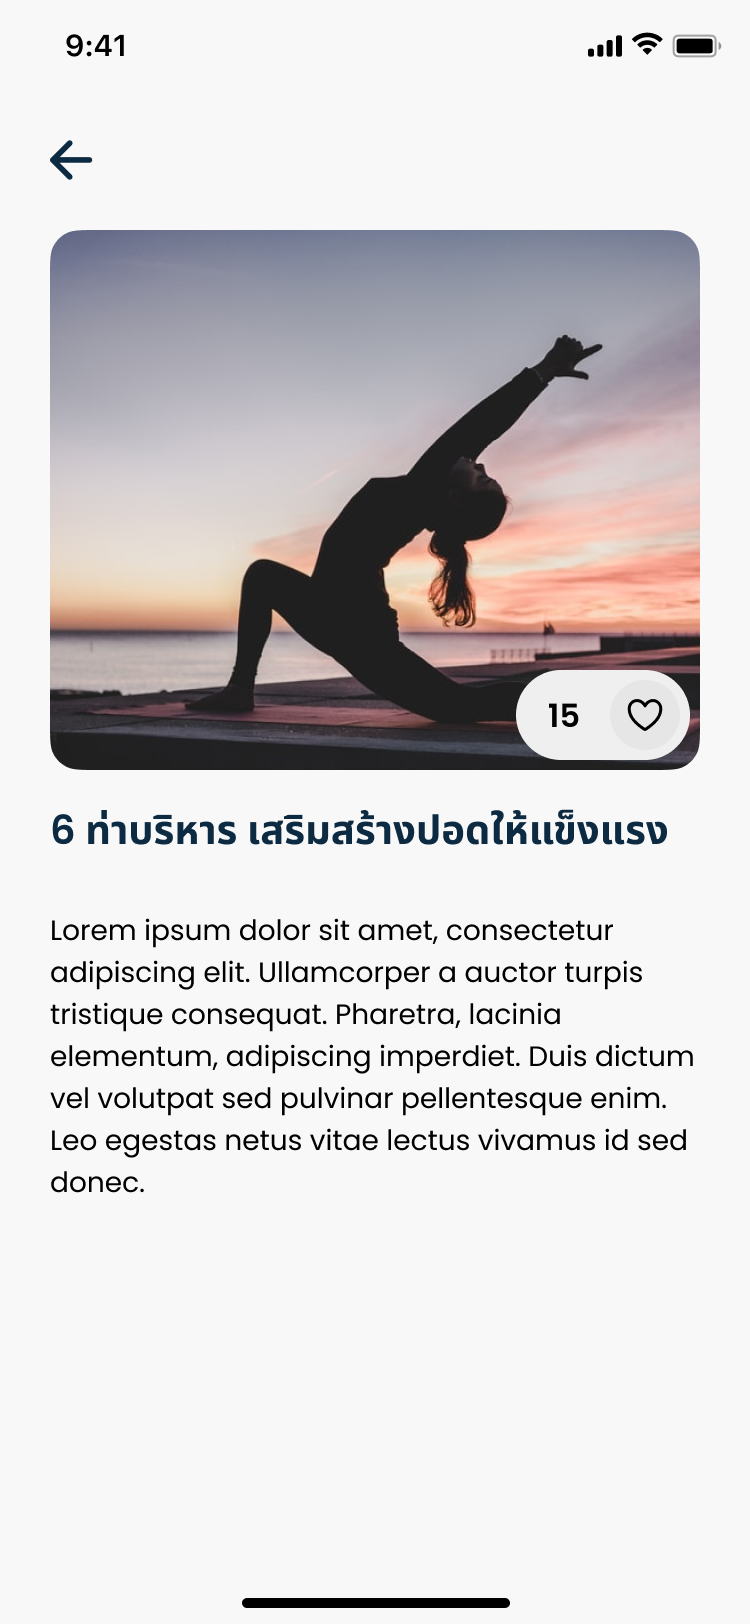
\includegraphics[height=10cm]{chapter_3/ui/News.png}
    \caption{หน้าข่าวสารของแอปพลิเคชัน}
\end{figure}

\subsection{หน้าการออกกำลังกาย}
หน้าการออกกำลังกาย ในหน้าแรกจะแสดงรายละเอียดคอร์ส รวมถึงคะแนนจากผู้ใช้ ระยะเวลาที่ใช้ และระดับความยากของคอร์ส เมื่อผู้ใช้กดปุ่มเริ่มการออกกำลังกาย ระบบจะแนะนำให้ผู้ใช้ทำท่าทางตามที่กำหนด โดยจะมีรายละเอียดแสดงอยู่ทางด้านบน และจะมีการแสดงข้อความแนะนำการปรับปรุงท่าทางการออกกำลังกายให้แก่ผู้ใช้
\begin{figure}
    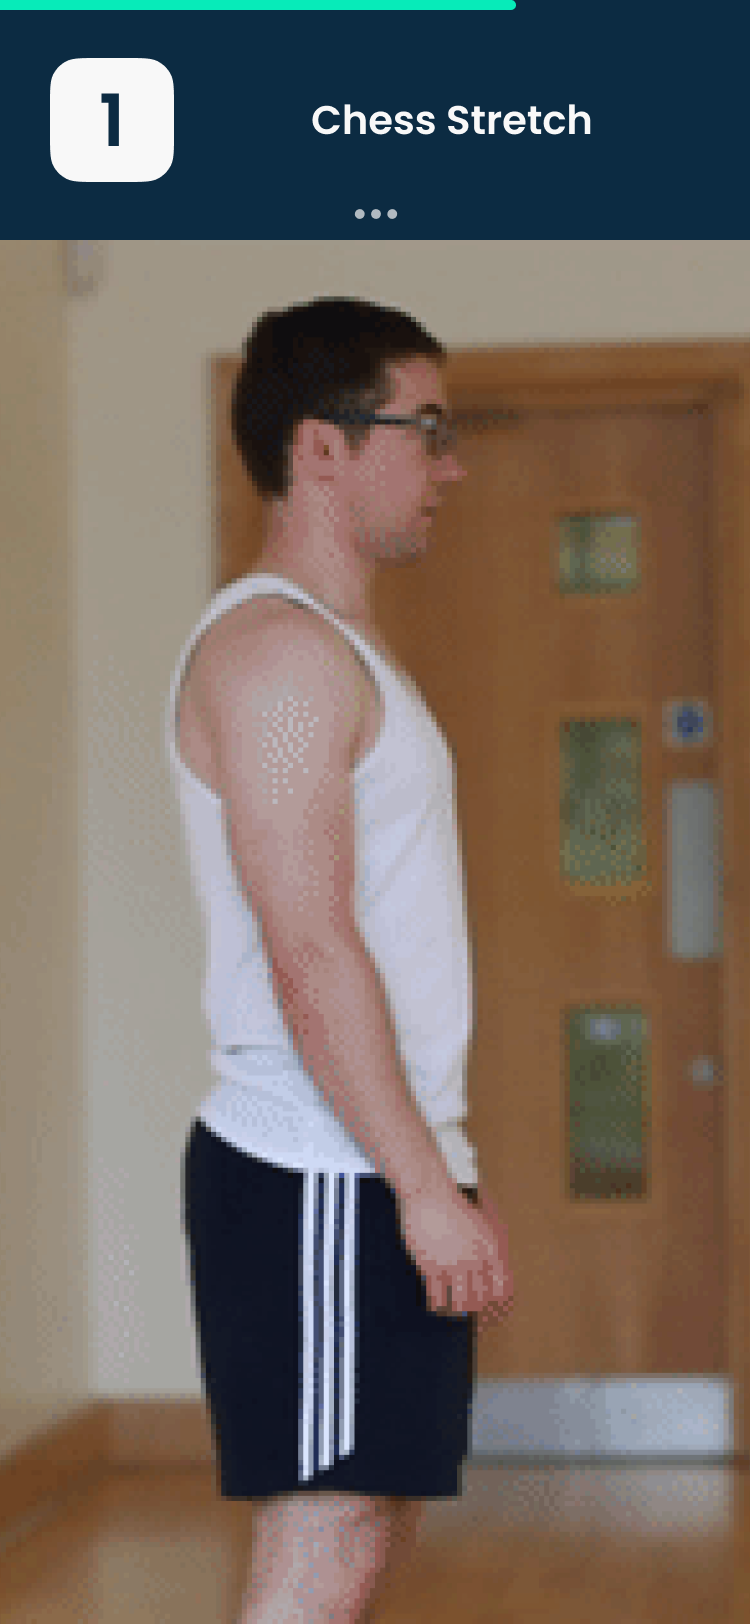
\includegraphics[height=10cm]{chapter_3/ui/Exercise/Step Begin.png}
    \caption{หน้าการสอนท่าทางให้แก่ผู้ใช้}
\end{figure}

\begin{figure}
    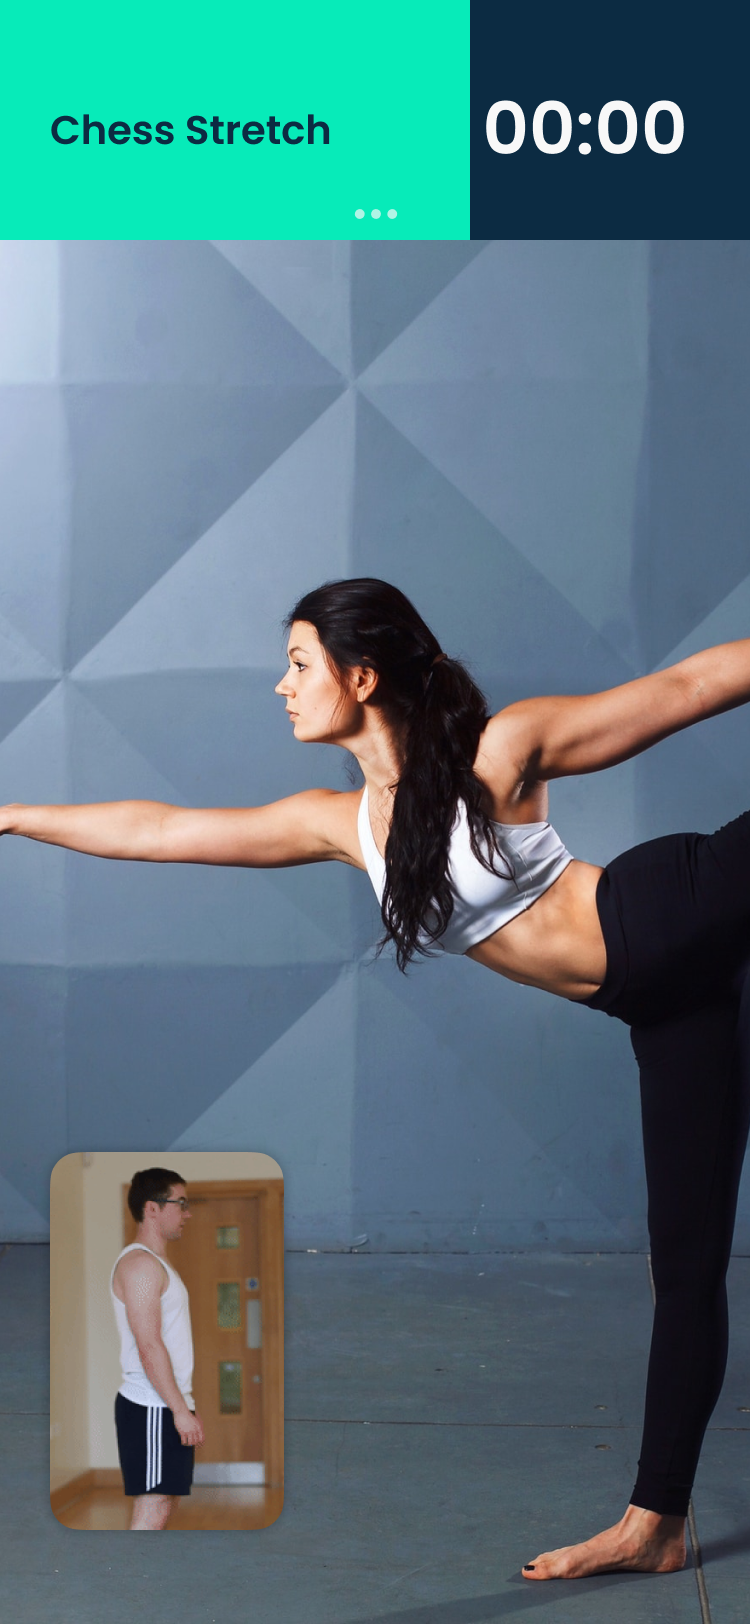
\includegraphics[height=10cm]{chapter_3/ui/Exercise/Step Counting.png}
    \caption{หน้าการออกกำลังกายที่จับเวลาให้ผู้ใช้ออกท่าทางค้างไว้ในเวลาที่กำหนด}
\end{figure}

\begin{figure}
    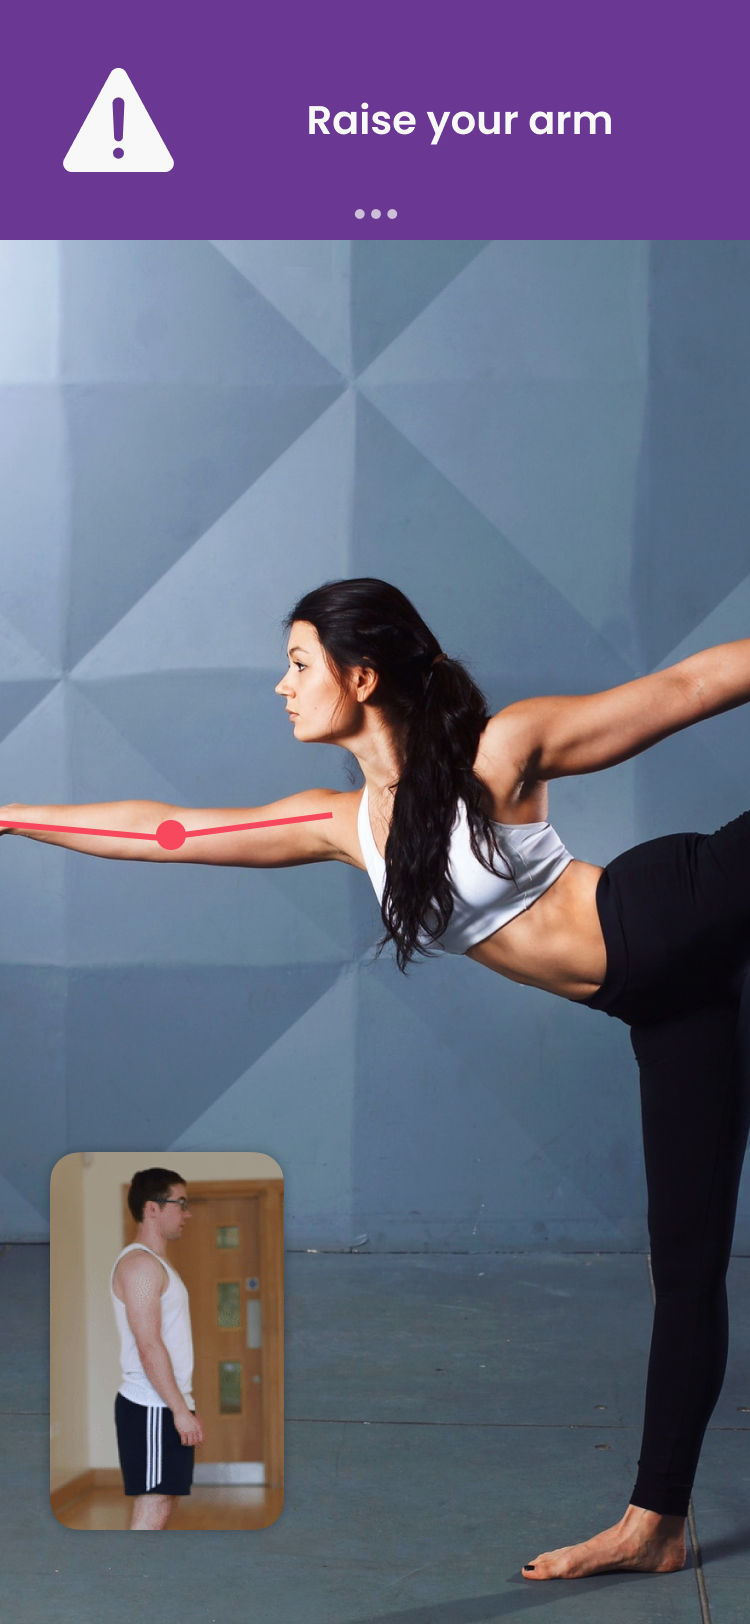
\includegraphics[height=10cm]{chapter_3/ui/Exercise/Warning.png}
    \caption{หน้าการแนะนำการปรับปรุงท่าทางให้แก่ผู้ใช้}
\end{figure}

\begin{figure}
    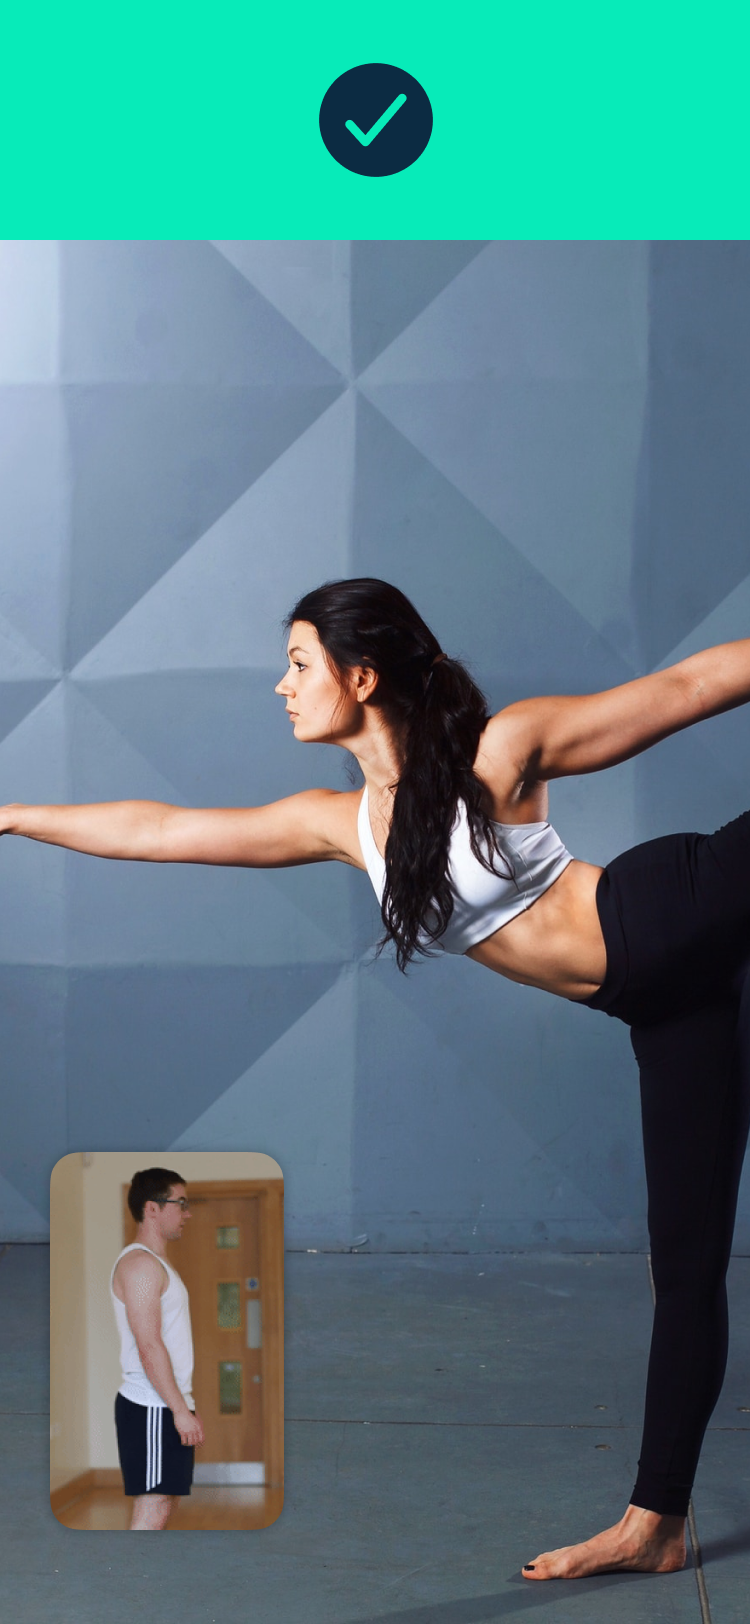
\includegraphics[height=10cm]{chapter_3/ui/Exercise/Step Finish.png}
    \caption{หน้าเมื่อเสร็จสิ้นการออกกำลังกาย}
\end{figure}

\subsection{หน้าบัญชีผู้ใช้}
หน้าบัญชีของผู้ใช้ ให้ผู้ใช้สามารถดูข้อมูลส่วนตัวของตนเองได้ รวมถึงดูเหรียญรางวัลเสมือนของตนเองได้

\begin{figure}
    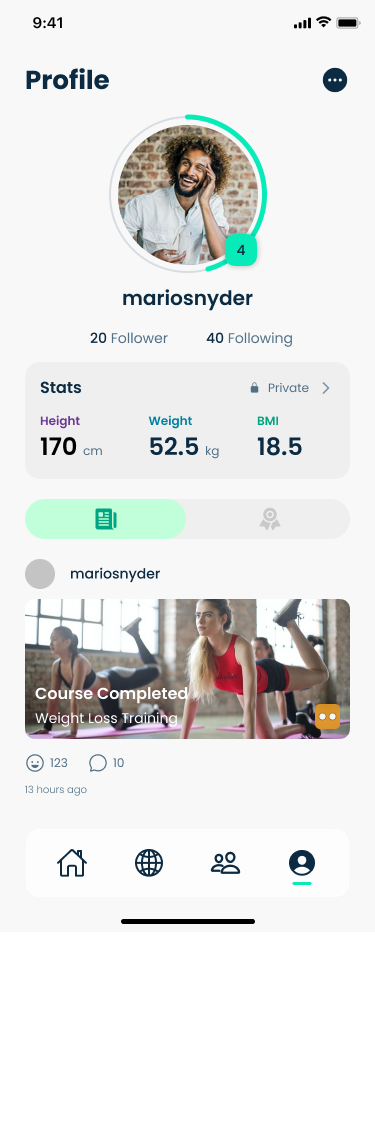
\includegraphics[height=10cm]{chapter_3/ui/Profile.png}
    \caption{หน้าบัญชีของผู้ใช้}
\end{figure}


\clearpage

\section{การออกแบบส่วนโครงสร้างระบบฐานข้อมูล (Database Schema)}
การออกแบบส่วนโครงสร้างระบบฐานข้อมูล (Database Schema) ดังนี้
\begin{figure}
    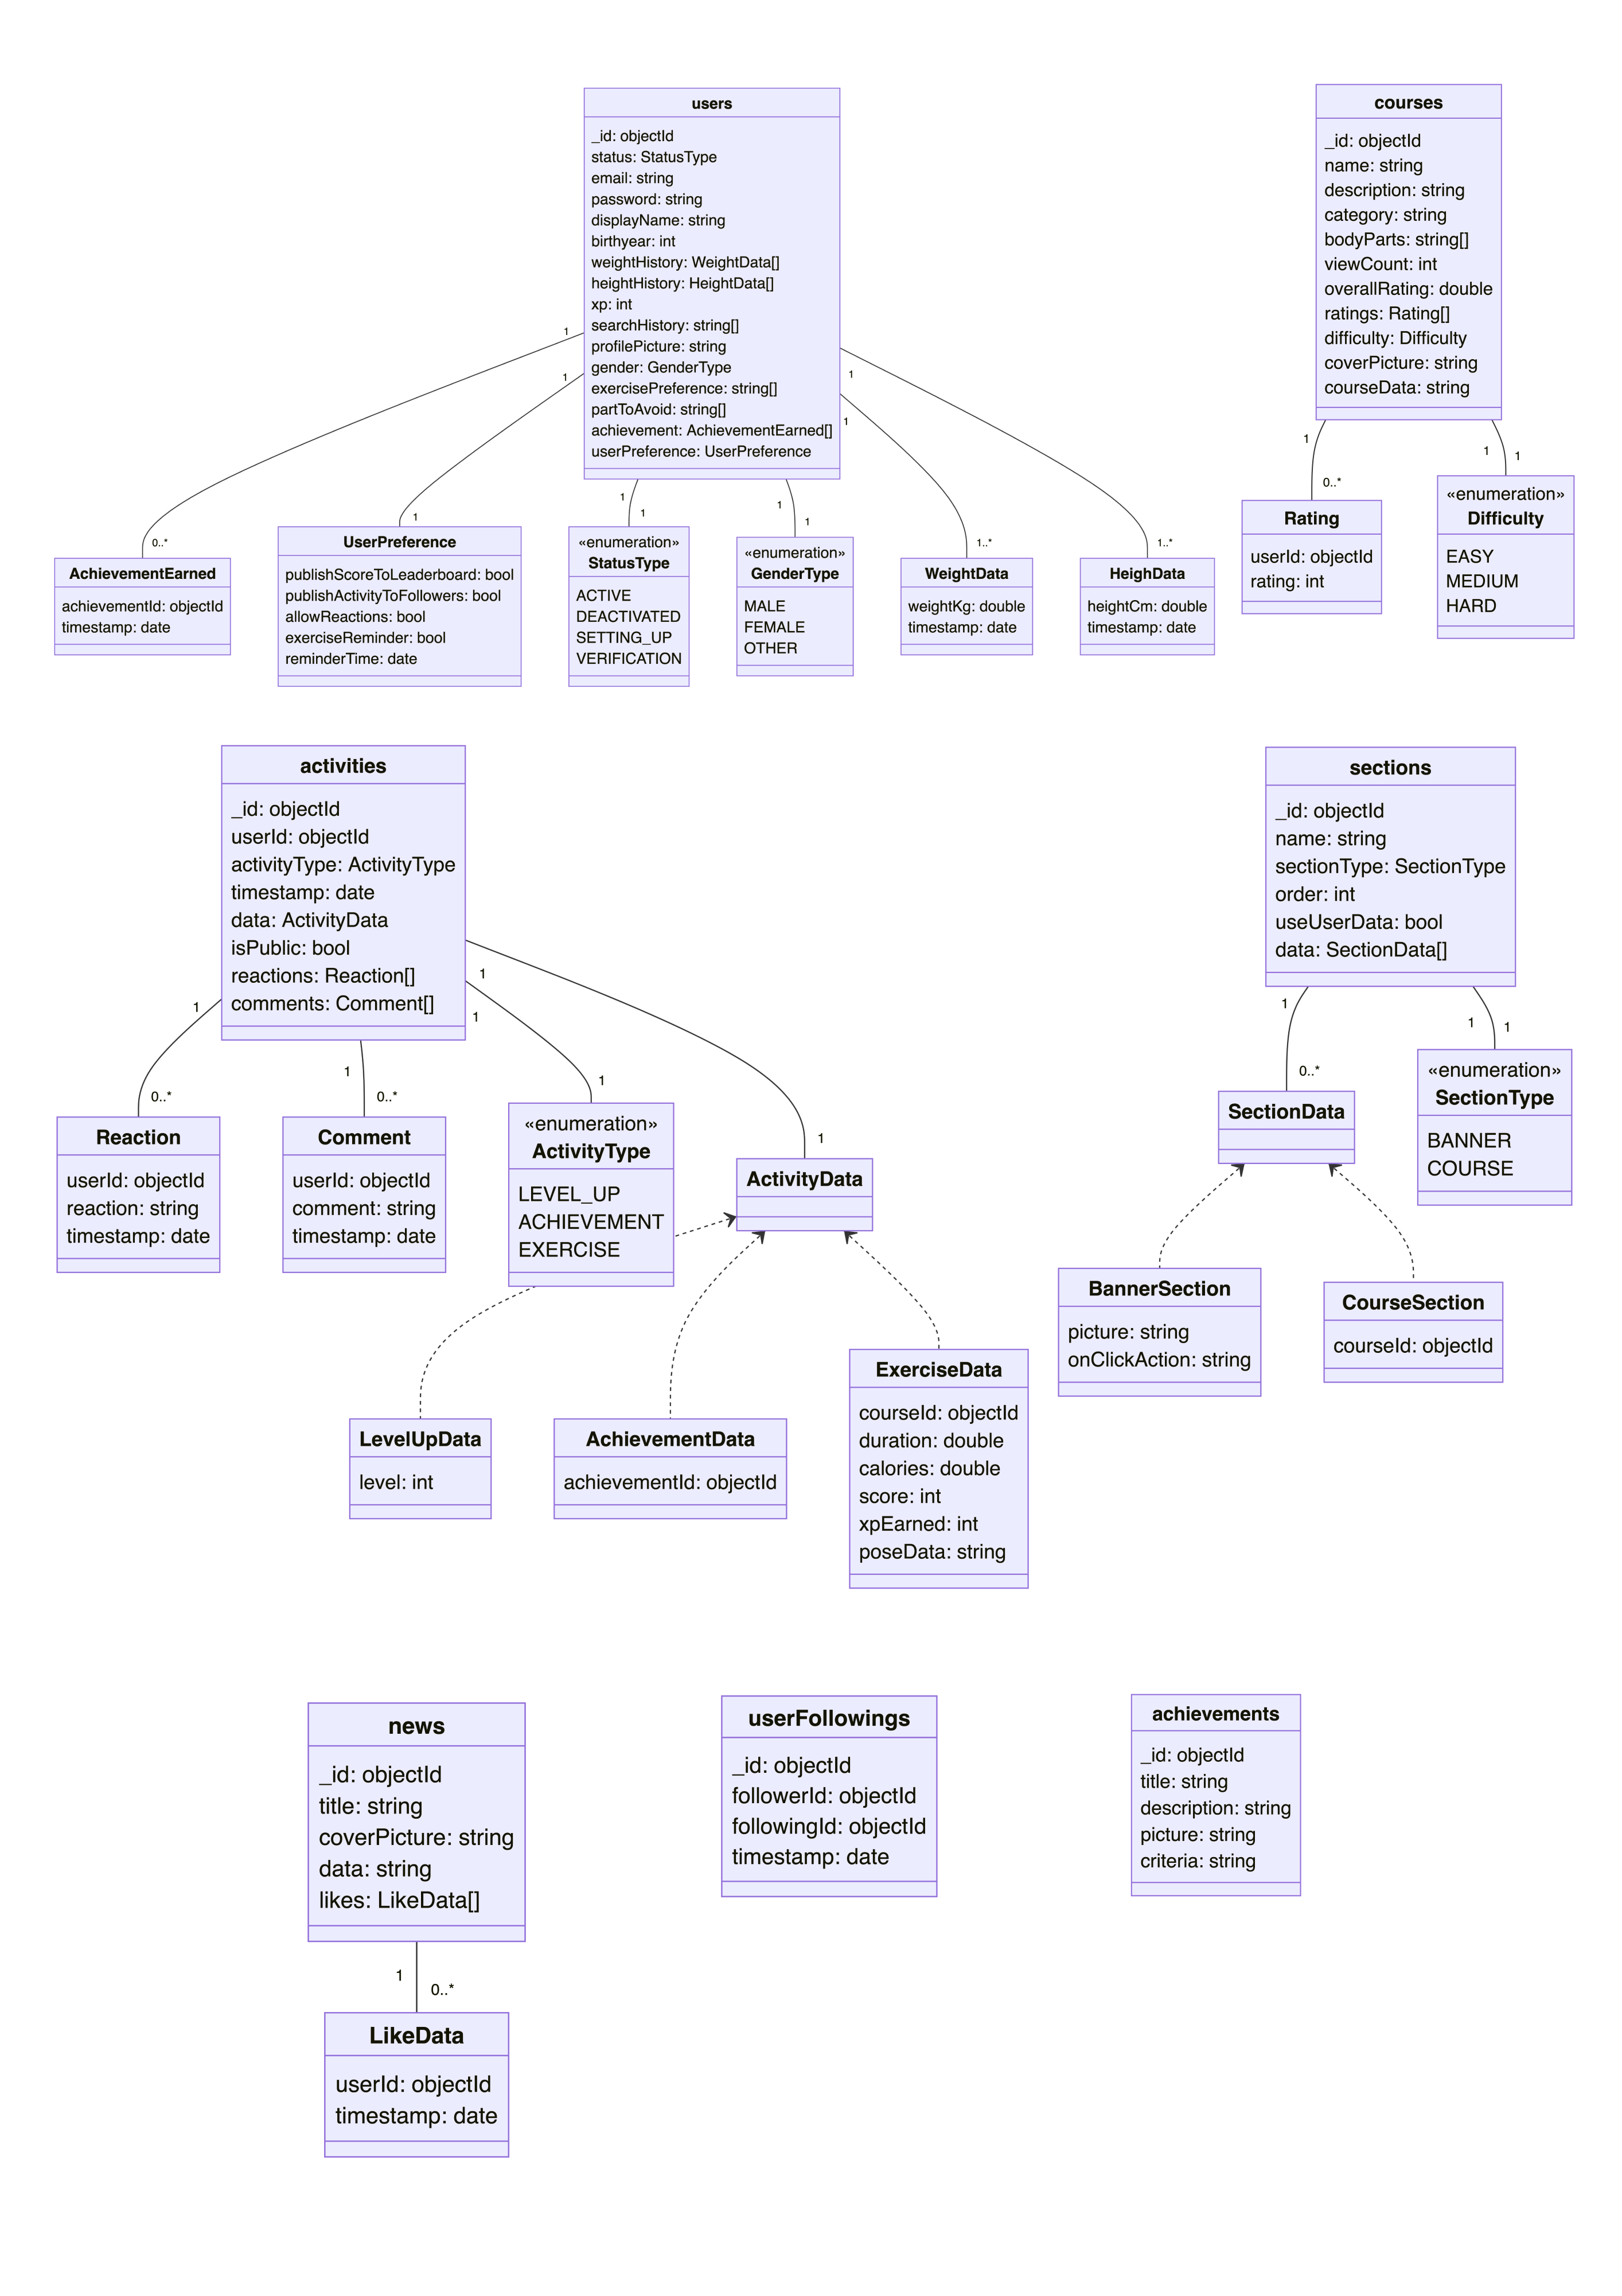
\includegraphics[width=\textwidth]{chapter_3/database.png}
    \caption{การออกแบบโครงสร้างฐานข้อมูล}
    \label{fig:db-schema}
\end{figure}
\clearpage
การออกแบบฐานข้อมูลตามรูปที่ \ref{fig:db-schema} มีรายละเอียดดังต่อไปนี้

\begin{table}
    \caption{รายละเอียดฐานข้อมูลในคอลเล็กชัน users}
    \begin{tabularx}{\textwidth}{ | l | l | X | }
        \hline
        \bf ชื่อแอตทริบิวต์ & \bf ชนิดตัวแปร & \bf รายละเอียด \\\hline
        \_ id & objectId & ID ของ document ใน collection users\\\hline
        status & StatusType & สถานะของบัญชีผู้ใช้\\\hline
        email & string & อีเมลของผู้ใช้\\\hline
        password & string & รหัสผ่านของผู้ใช้\\\hline
        displayName & string & ชื่อ Display Name ของผู้ใช้\\\hline
        birthyear & int & ปีเกิดของผู้ใช้\\\hline
        weightHistory & WeightData[] & ประวัติน้ำหนักของผู้ใช้\\\hline
        heightHistory & HeightData[] & ประวัติส่วนสูงของผู้ใช้\\\hline
        xp & int & คะแนนของผู้ใช้\\\hline
        level & int & ขั้น (Level) ของผู้ใช้\\\hline
        profilePicture & string & URL รูปภาพโปรไฟล์ของผู้ใช้\\\hline
        gender & GenderType & เพศของผู้ใช้\\\hline
        exercisePreference & string[] & รายการประเภทการออกกำลังกายที่ชอบ\\\hline
        partToAvoid & string[] & รายการสัดส่วนของผู้ใช้ที่ต้องการหลีกเลี่ยง\\\hline
    \end{tabularx}
\end{table}

\begin{table}
    \caption{รายละเอียดชนิดตัวแปร AchievementEarned}
    \begin{tabularx}{\textwidth}{ | l | l | X | }
        \hline
        \bf ชื่อแอตทริบิวต์ & \bf ชนิดตัวแปร & \bf รายละเอียด \\\hline
        achievementId & objectId & ID ของเหรียญรางวัลเสมือน\\\hline
        timestamp & date & วันและเวลาที่ผู้ใช้ได้รับเหรียญ\\\hline 
    \end{tabularx}
\end{table}

\begin{table}
    \caption{รายละเอียดชนิดตัวแปร UserPreference}
    \begin{tabularx}{\textwidth}{ | l | l | X | }
        \hline
        \bf ชื่อแอตทริบิวต์ & \bf ชนิดตัวแปร & \bf รายละเอียด \\\hline
        publishScoreToLeaderboard & bool & เผยแพร่คะแนนของผู้ใช้บนตารางลีดเดอร์บอร์ด\\\hline
        publishActivityToFollowers & bool & เผยแพร่กิจกรรมของผู้ใช้ไปยังคนที่กำลังติดตามผู้ใช้\\\hline
        allowReactions & bool & ให้ผู้อื่นสามารถกด Reaction กับกิจกรรมได้\\\hline
        exerciseReminder & bool & การแจ้งเตือนให้ออกกำลังกาย\\\hline
        reminderTime & date & เวลาที่ผู้ใช้ต้องการให้เตือนเพือออกกำลังกาย\\\hline
    \end{tabularx}
\end{table}

\begin{table}
    \caption{รายละเอียด Enumeration StatusType}
    \begin{tabularx}{\textwidth}{ | l | X | }
        \hline
        \bf ชื่อแอตทริบิวต์ & \bf รายละเอียด \\\hline
        ACTIVE & บัญชีผู้ใช้มีสถานะปกติ\\\hline
        DEACTIVATED & บัญชีผู้ใช้มีสถานะปิดบัญชี\\\hline
        SETTING\_UP & บัญชีผู้ใช้มีสถานะกำลังอยู่ในขั้นตอนการตั้งค่าผู้ใช้ใหม่\\\hline
        VERIFICATION & บัญชีผู้ใช้มีสถานะกำลังรอการยืนยันอีเมล\\\hline
    \end{tabularx}
\end{table}

\begin{table}
    \caption{รายละเอียด Enumeration GenderType}
    \begin{tabularx}{\textwidth}{ | l | X | }
        \hline
        \bf ชื่อแอตทริบิวต์ & \bf รายละเอียด \\\hline
        MALE & เพศของผู้ใช้คือเพศชาย\\\hline
        FEMALE & เพศของผู้ใช้คือเพศหญิง\\\hline
        OTHER & เพศของผู้ใช้คืออื่น ๆ\\\hline
    \end{tabularx}
\end{table}

\begin{table}
    \caption{รายละเอียดชนิดตัวแปร WeightData}
    \begin{tabularx}{\textwidth}{ | l | l | X | }
        \hline
        \bf ชื่อแอตทริบิวต์ & \bf ชนิดตัวแปร & \bf รายละเอียด \\\hline
        weightKg & double & น้ำหนักของผู้ใช้ (หน่วยกิโลกรัม)\\\hline
        timestamp & date & วันที่และเวลาที่ผู้ใช้กรอกข้อมูล\\\hline
    \end{tabularx}
\end{table}

\begin{table}
    \caption{รายละเอียดชนิดตัวแปร HeightData}
    \begin{tabularx}{\textwidth}{ | l | l | X | }
        \hline
        \bf ชื่อแอตทริบิวต์ & \bf ชนิดตัวแปร & \bf รายละเอียด \\\hline
        heightCm & double & ส่วนสูงของผู้ใช้ (หน่วยเซนติเมตร)\\\hline
        timestamp & date & วันที่และเวลาที่ผู้ใช้กรอกข้อมูล\\\hline
    \end{tabularx}
\end{table}

\begin{table}
    \caption{รายละเอียดฐานข้อมูลใน collection courses}
    \begin{tabularx}{\textwidth}{ | l | l | X | }
        \hline
        \bf ชื่อแอตทริบิวต์ & \bf ชนิดตัวแปร & \bf รายละเอียด \\\hline
        \_id & objectId & ID ของ document ใน collection courses\\\hline
        name & string & ชื่อคอร์ส\\\hline
        description & string & คำอธิบายของคอร์ส\\\hline
        category & string & หมวดหมู่คอร์ส\\\hline
        bodyParts & string[] & ส่วนของร่างกายที่ต้องใช้\\\hline
        viewCount & int & จำนวนการเข้าดูคอร์สนี้\\\hline
        rating & Rating[] & รายการของผู้ใช้ที่ให้คะแนนกับคอร์สนี้\\\hline
        difficulty & Difficulty & ความยาก-ง่ายของคอร์ส\\\hline
        coverPicture & string & URL รูปภาพหน้าปกคอร์ส\\\hline
        courseData & string & URL ไฟล์ข้อมูลท่าทางการออกกำลังกาย\\\hline
    \end{tabularx}
\end{table}

\begin{table}
    \caption{รายละเอียดชนิดตัวแปร Rating}
    \begin{tabularx}{\textwidth}{ | l | l | X | }
        \hline
        \bf ชื่อแอตทริบิวต์ & \bf ชนิดตัวแปร & \bf รายละเอียด \\\hline
        userId & objectId & ID ของผู้ใช้ที่ให้คะแนน\\\hline
        rating & int & คะแนนที่ผู้ใช้ให้\\\hline
    \end{tabularx}
\end{table}

\begin{table}
    \caption{รายละเอียด Enumeration Difficulty}
    \begin{tabularx}{\textwidth}{ | l | X | }
        \hline
        \bf ชื่อแอตทริบิวต์ & \bf รายละเอียด \\\hline
        EASY & คอร์สระดับง่าย\\\hline
        MEDIUM & คอร์สระดับปานกลาง\\\hline
        HARD & คอร์สระดับยาก\\\hline
    \end{tabularx}
\end{table}

\begin{table}
    \caption{รายละเอียดฐานข้อมูลในคอลเล็กชัน achievements}
    \begin{tabularx}{\textwidth}{ | l | l | X | }
        \hline
        \bf ชื่อแอตทริบิวต์ & \bf ชนิดตัวแปร & \bf รายละเอียด \\\hline
        \_id & objectId & ID ของเหรียญรางวัลเสมือน\\\hline
        title & string & ชื่อของเหรียญรางวัลเสมือน\\\hline
        description & string & คำอธิบายเหรียญรางวัลเสมือน\\\hline
        picture & string & รูปภาพของเหรียญรางวัลเสมือน\\\hline
        criteria & string[] & รายการเกณฑ์ต่าง ๆ ของเหรียญรางวัลเสมือน\\\hline
    \end{tabularx}
\end{table}

\begin{table}
    \caption{รายละเอียดฐานข้อมูลในคอลเล็กชัน activities}
    \begin{tabularx}{\textwidth}{ | l | l | X | }
        \hline
        \bf ชื่อแอตทริบิวต์ & \bf ชนิดตัวแปร & \bf รายละเอียด \\\hline
        \_id & objectId & ID ของกิจกรรม\\\hline
        userId & objectId & ID ของผู้ใช้ที่เป็นผู้ทำกิจกรรม\\\hline
        activityType & ActivityType & ประเภทของกิจกรรม\\\hline
        timestamp & date & วันที่และเวลาที่ทำกิจกรรม\\\hline
        data & ActivityData & ข้อมูลรายละเอียดของกิจกรรม\\\hline
        isPublic & bool & ให้กิจกรรมนี้สามารถให้ผู้ที่ติดตามมองเห็นได้หรือไม่\\\hline
        reactions & Reaction[] & รายการผู้ใช้ที่กดแสดงความรู้สึก (Reaction) ต่อกิจกรรมนี้\\\hline
        comments & Comment[] & รายการที่ผู้ใช้แสดงความคิดเห็น (Comment) ต่อกิจกรรมนี้\\\hline
    \end{tabularx}
\end{table}

\begin{table}
    \caption{รายละเอียดชนิดตัวแปร LevelUpData}
    \begin{tabularx}{\textwidth}{ | l | l | X | }
        \hline
        \bf ชื่อแอตทริบิวต์ & \bf ชนิดตัวแปร & \bf รายละเอียด \\\hline
        level & int & ระดับ (Level) ที่ผู้ใช้ได้รับ\\\hline
    \end{tabularx}
\end{table}

\begin{table}
    \caption{รายละเอียดชนิดตัวแปร ExerciseData}
    \begin{tabularx}{\textwidth}{ | l | l | X | }
        \hline
        \bf ชื่อแอตทริบิวต์ & \bf ชนิดตัวแปร & \bf รายละเอียด \\\hline
        courseId & objectId & ID ของคอร์สที่ผู้ใช้ได้ออกกำลังกาย\\\hline
        duration & double & ระยะเวลาที่ผู้ใช้เข้าคอร์ส (นาที)\\\hline
        calories & double & จำนวนแคลอรี่ที่ผู้ใช้ได้เผาผลาญไป\\\hline
        score & int & คะแนนความถูกต้องในการออกกำลังกายของผู้ใช้ (เป็นช่วงจาก 0 - 100)\\\hline
        xpEarned & int & คะแนนที่ผู้ใช้ได้รับ\\\hline
        poseData & string & URL ไฟล์ข้อมูลท่าทางของผู้ใช้\\\hline
    \end{tabularx}
\end{table}

\begin{table}
    \caption{รายละเอียด Enumeration ActivityType}
    \begin{tabularx}{\textwidth}{ | l | X | }
        \hline
        \bf ชื่อแอตทริบิวต์ & \bf รายละเอียด \\\hline
        LEVEL\_UP & กิจกรรม ประเภทการเลื่อนระดับ\\\hline
        ACHIEVEMENT & กิจกรรม ประเภทที่ได้รับเหรียญรางวัลเสมือน\\\hline
        EXERCISE & กิจกรรม ประเภทการออกกำลังกาย\\\hline
    \end{tabularx}
\end{table}

\begin{table}
    \caption{รายละเอียดชนิดตัวแปร Reaction}
    \begin{tabularx}{\textwidth}{ | l | l | X | }
        \hline
        \bf ชื่อแอตทริบิวต์ & \bf ชนิดตัวแปร & \bf รายละเอียด \\\hline
        \_id & objectId & ID ของกิจกรรม\\\hline
        userId & objectId & ID ของผู้ใช้ที่ได้แสดงความรู้สึก (Reaction)\\\hline
        reaction & string & ชื่อความรู้สึก (Reaction)\\\hline
        timestamp & date & วันที่และเวลาที่ได้กดแสดงความรู้สึก (Reaction)\\\hline
    \end{tabularx}
\end{table}

\begin{table}
    \caption{รายละเอียดชนิดตัวแปร Comment}
    \begin{tabularx}{\textwidth}{ | l | l | X | }
        \hline
        \bf ชื่อแอตทริบิวต์ & \bf ชนิดตัวแปร & \bf รายละเอียด \\\hline
        \_id & objectId & ID ของกิจกรรม\\\hline
        userId & objectId & ID ของผู้ใช้ที่ได้แสดงความคิดเห็น\\\hline
        comment & string & ความคิดเห็นของผู้ใช้\\\hline
        timestamp & date & วันที่และเวลาที่ได้แสดงความคิดเห็น\\\hline
    \end{tabularx}
\end{table}

\begin{table}
    \caption{รายละเอียดฐานข้อมูลในคอลเล็กชัน news}
    \begin{tabularx}{\textwidth}{ | l | l | X | }
        \hline
        \bf ชื่อแอตทริบิวต์ & \bf ชนิดตัวแปร & \bf รายละเอียด \\\hline
        \_id & objectId & ID ของข่าวสาร\\\hline
        title & string & หัวเรื่องของข่าวสาร\\\hline
        coverPicture & string & URL รูปภาพหน้าปก\\\hline
        data & string & URL ไฟล์ข้อมูลของข่าวสาร\\\hline
        likes & LikeData[] & รายการผู้ที่กดชื่นชอบข่าว\\\hline
    \end{tabularx}
\end{table}

\begin{table}
    \caption{รายละเอียดชนิดตัวแปร LikeData}
    \begin{tabularx}{\textwidth}{ | l | l | X | }
        \hline
        \bf ชื่อแอตทริบิวต์ & \bf ชนิดตัวแปร & \bf รายละเอียด \\\hline
        userId & objectId & ID ของผู้ใช้\\\hline
        timestamp & date & วันและเวลาที่ผู้ใช้กดชื่นชอบ\\\hline
    \end{tabularx}
\end{table}

\begin{table}
    \caption{รายละเอียดฐานข้อมูลในคอลเล็กชัน sections}
    \noindent ใช้ในการเก็บข้อมูลส่วนต่าง ๆ ในหน้าหลัก (Home) ที่จะมีการแนะนำคอร์สต่าง ๆ
    \begin{tabularx}{\textwidth}{ | l | l | X | }
        \hline
        \bf ชื่อแอตทริบิวต์ & \bf ชนิดตัวแปร & \bf รายละเอียด \\\hline
        \_id & objectId & ID ของส่วน\\\hline
        name & string & ชื่อของส่วนนี้\\\hline
        sectionType & SectionType & ประเภทของส่วน\\\hline
        order & int & ลำดับของส่วนบนหน้าหลัก\\\hline
        useUserData & bool & นำข้อมูลของผู้ใช้มาประกอบการแนะนำหรือไม่\\\hline
        data & SectionData[] & ข้อมูลของส่วน\\\hline
    \end{tabularx}
\end{table}

\begin{table}
    \caption{รายละเอียดชนิดคลาส BannerSection}
    \noindent ใช้ในการเก็บข้อมูลส่วนต่าง ๆ ในหน้าหลัก (Home) ที่จะมีการแนะนำคอร์สต่าง ๆ
    \begin{tabularx}{\textwidth}{ | l | l | X | }
        \hline
        \bf ชื่อแอตทริบิวต์ & \bf ชนิดตัวแปร & \bf รายละเอียด \\\hline
        picture & string & URL ไฟล์รูปภาพ\\\hline
        onClickAction & string & กำหนดการกระทำเมื่อผู้ใช้กดไปยัง Banner\\\hline
    \end{tabularx}
\end{table}

\begin{table}
    \caption{รายละเอียดชนิดคลาส CourseSection}
    \begin{tabularx}{\textwidth}{ | l | l | X | }
        \hline
        \bf ชื่อแอตทริบิวต์ & \bf ชนิดตัวแปร & \bf รายละเอียด \\\hline
        courseId & objectId & คอร์สที่แนะนำ\\\hline
    \end{tabularx}
\end{table}

\begin{table}
    \caption{รายละเอียด Enumeration SectionType}
    \begin{tabularx}{\textwidth}{ | l | X | }
        \hline
        \bf ชื่อแอตทริบิวต์ & \bf รายละเอียด \\\hline
        BANNER & ส่วนเป็นแบบ Banner\\\hline
        COURSE & ส่วนเป็นแบบ Course\\\hline
    \end{tabularx}
\end{table}

\begin{table}
    \caption{รายละเอียดฐานข้อมูลในคอลเล็กชัน userFollowings}
    \begin{tabularx}{\textwidth}{ | l | l | X | }
        \hline
        \bf ชื่อแอตทริบิวต์ & \bf ชนิดตัวแปร & \bf รายละเอียด \\\hline
        \_id & objectId & ID ของรายการบันทึกการติดตามของผู้ใช้\\\hline
        followerId & objectId & ID ของผู้ใช้ที่กดติดตาม\\\hline
        followingId & objectId & ID ของผู้ใช้ที่ถูกติดตาม\\\hline
        timestamp & date & วันและเวลาที่ผู้ใช้ได้กดติดตาม\\\hline
    \end{tabularx}
\end{table}

\clearpage


\section{การออกแบบส่วนการวิเคราะห์ ตรวจสอบ และแนะนำท่าทางของผู้ใช้}
ในการออกแบบส่วนการวิเคราะห์ ตรวจสอบ และแนะนำท่าทางของผู้ใช้ จะแสดงเป็นแผนภาพการทำงานระหว่างระบบต่าง ๆ ได้ ดังนี้
\begin{figure}
    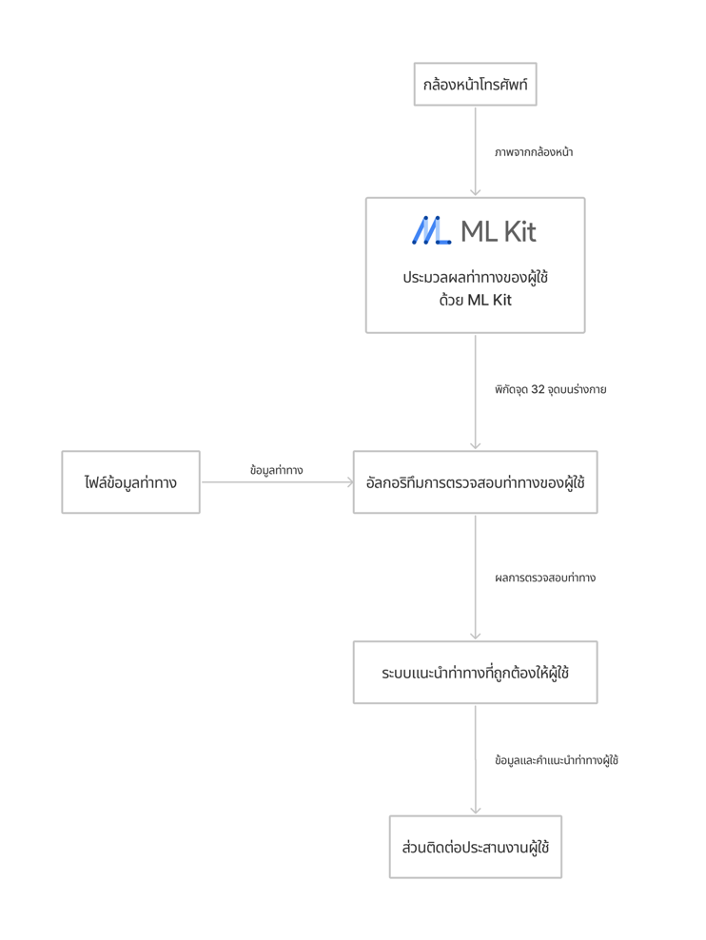
\includegraphics[width=\textwidth - 2cm]{chapter_3/pose overview.png}
    \caption{ภาพรวมระบบการวิเคราะห์ ตรวจสอบ และแนะนำท่าทางของผู้ใช้}
\end{figure}
จากแผนภาพข้างต้น สามารถอธิบายออกเป็นส่วนต่าง ๆ ซึ่งจะแบ่งออกเป็น 4 ส่วน คือ ส่วนการประมวลผลท่าทางของผู้ใช้ด้วย ML Kit, ส่วนไฟล์ข้อมูลท่าทาง, ส่วนอัลกอริทึมการตรวจสอบท่าทางของผู้ใช้ และส่วนระบบแนะนำท่าทางที่ถูกต้องให้ผู้ใช้

\subsection{ส่วนการประมวลผลท่าทางของผู้ใช้ด้วย ML Kit}
สำหรับระบบการวิเคราะห์ท่าทาง จะใช้ API ของ ML Kit ในการตรวจจับท่าทางของผู้ใช้ ซึ่งจะได้พิกัดจุดทั้งหมด 32 จุดทั่วร่างกาย
\begin{figure}
    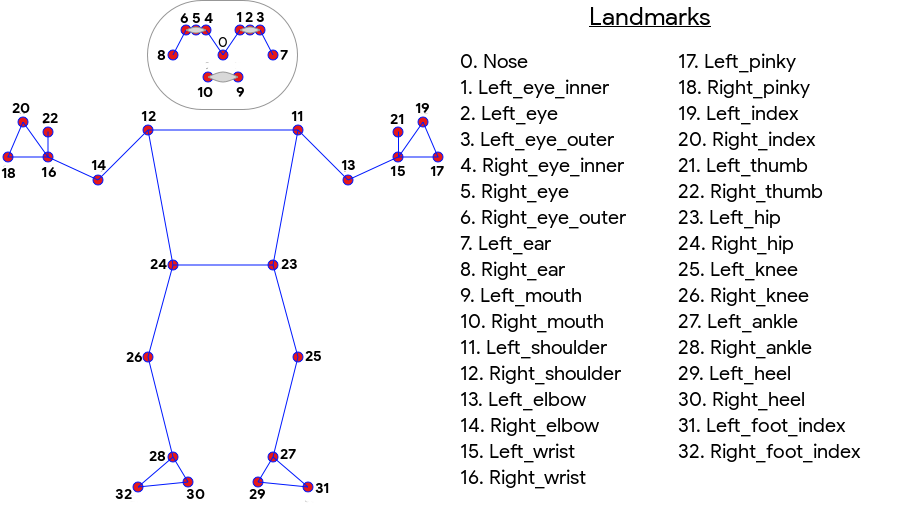
\includegraphics[width=\textwidth]{chapter_3/landmarks-fixed.png}
    \caption{แสดง Landmark จุดบนร่างกายที่ ML Kit สามารถตรวจจับได้}
\end{figure}

\subsection{ส่วนอัลกอริทึมการตรวจสอบท่าทางของผู้ใช้}
ในส่วนของการตรวจสอบท่าทางของผู้ใช้ ระบบจะนำข้อมูลพิกัดจุดที่ได้จากการประมวลผลในขั้นตอนที่แล้วมาใช้ โดยจะใช้ควบคู่กับไฟล์ข้อมูลท่าทางที่จะมีข้อมูลว่าจะต้องตรวจสอบท่าทางในจุดใดบ้าง ซึ่งจะประกอบไปด้วยคำสั่งที่จะให้ตรวจสอบ 2 คำสั่งคือ คำสั่งในการตรวจสอบองศาที่ทำมุมกันของจุดใด ๆ และคำสั่งตรวจสอบจุดใด ๆ ว่าอยู่ใกล้กันกับอีกจุดหนึ่งหรือไม่ โดยจะมีรายละเอียดในการหาผลลัพธ์ ดังนี้
\begin{enumerate}
    \item 	คำสั่งให้ตรวจสอบองศาของจุดที่ทำมุมกัน ในขั้นตอนแรกจะรับจุดทั้งหมด 3 จุด คือ จุด $A,B,C$ ซึ่งจะให้จุด $A$ เป็นจุดเริ่มต้น จากนั้นจึงคำนวณเวกเตอร์สามมิติซึ่งจะได้ออกมาเป็นเวกเตอร์ $\overrightarrow{AB}$ และ เวกเตอร์ $\overrightarrow{AC}$ ดังรูปภาพตัวอย่าง
    \begin{figure}
        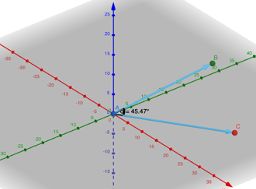
\includegraphics[width=7cm]{chapter_3/vector ex.png}
        \caption{แสดงตัวอย่างการหาเวกเตอร์ที่มีจุด A เป็นจุดร่วม}
    \end{figure}
    จากนั้นจึงหาองศาระหว่างเวกเตอร์ทั้งสองได้ จากสมการ
    \begin{equation}
        \alpha = \arccos{\left( \frac{\overrightarrow{AB} \cdot \overrightarrow{AC}}{|\overrightarrow{AB}| \cdot |\overrightarrow{AC}|} \right)}
    \end{equation}
    และเมื่อได้องศาเรียบร้อยแล้ว จึงจะนำไปตรวจสอบกับค่าที่ได้รับว่าตรงตามที่ได้กำหนดไว้หรือไม่ ซึ่งในส่วนนี้ได้กำหนดค่าความคลาดเคลื่อนเริ่มต้นที่ 10 องศา แต่สามารถเปลี่ยนแปลงได้ถ้ามีการระบุไว้ในไฟล์ข้อมูลท่าทาง
    \item คำสั่งตรวจสอบจุดใด ๆ ว่าอยู่ใกล้กันกับอีกจุดหนึ่งหรือไม่ จะรับจุดจำนวน 2 จุด แล้วทำการคำนวณว่าจุดที่ได้รับ อยู่ใกล้เคียงกันหรือไม่ โดยการสร้างทรงกลมขึ้นมาโดยให้จุดที่ได้รับเป็นจุดศูนย์กลาง จะได้ทรงกลมขึ้นมาทั้งหมด 2 ลูกที่รัศมีเท่า ๆ กัน แล้วจึงทำการคำนวณว่าทรงกลมนี้มีการทับกันบางส่วนหรือทั้งหมดหรือไม่ โดยถ้ามีการทับกันจะถือว่าจุดทั้งสองอยู่ใกล้เคียงกัน
\end{enumerate}

\subsection{ส่วนไฟล์ข้อมูลท่าทาง}
ไฟล์ข้อมูลท่าทาง จะเป็นไฟล์ที่รวบรวมข้อมูลท่าทางทั้งหมดของทั้งคอร์ส ซึ่งภายในจะประกอบไปด้วยข้อมูลลำดับของท่าทาง, วิธีการนับท่าทางเป็นการจับเวลาหรือการนับการกระทำซ้ำ, ที่อยู่ของสื่อที่จะนำมาใช้สอนผู้ใช้ และเกณฑ์ต่าง ๆ ที่จะต้องตรวจสอบท่าทางนั้น ๆ และจะใช้ภาษา YAML ในการใช้งาน ซึ่งจะแสดงโครงสร้างไฟล์เป็น UML Class Diagram ได้ดังนี้

\begin{figure}
    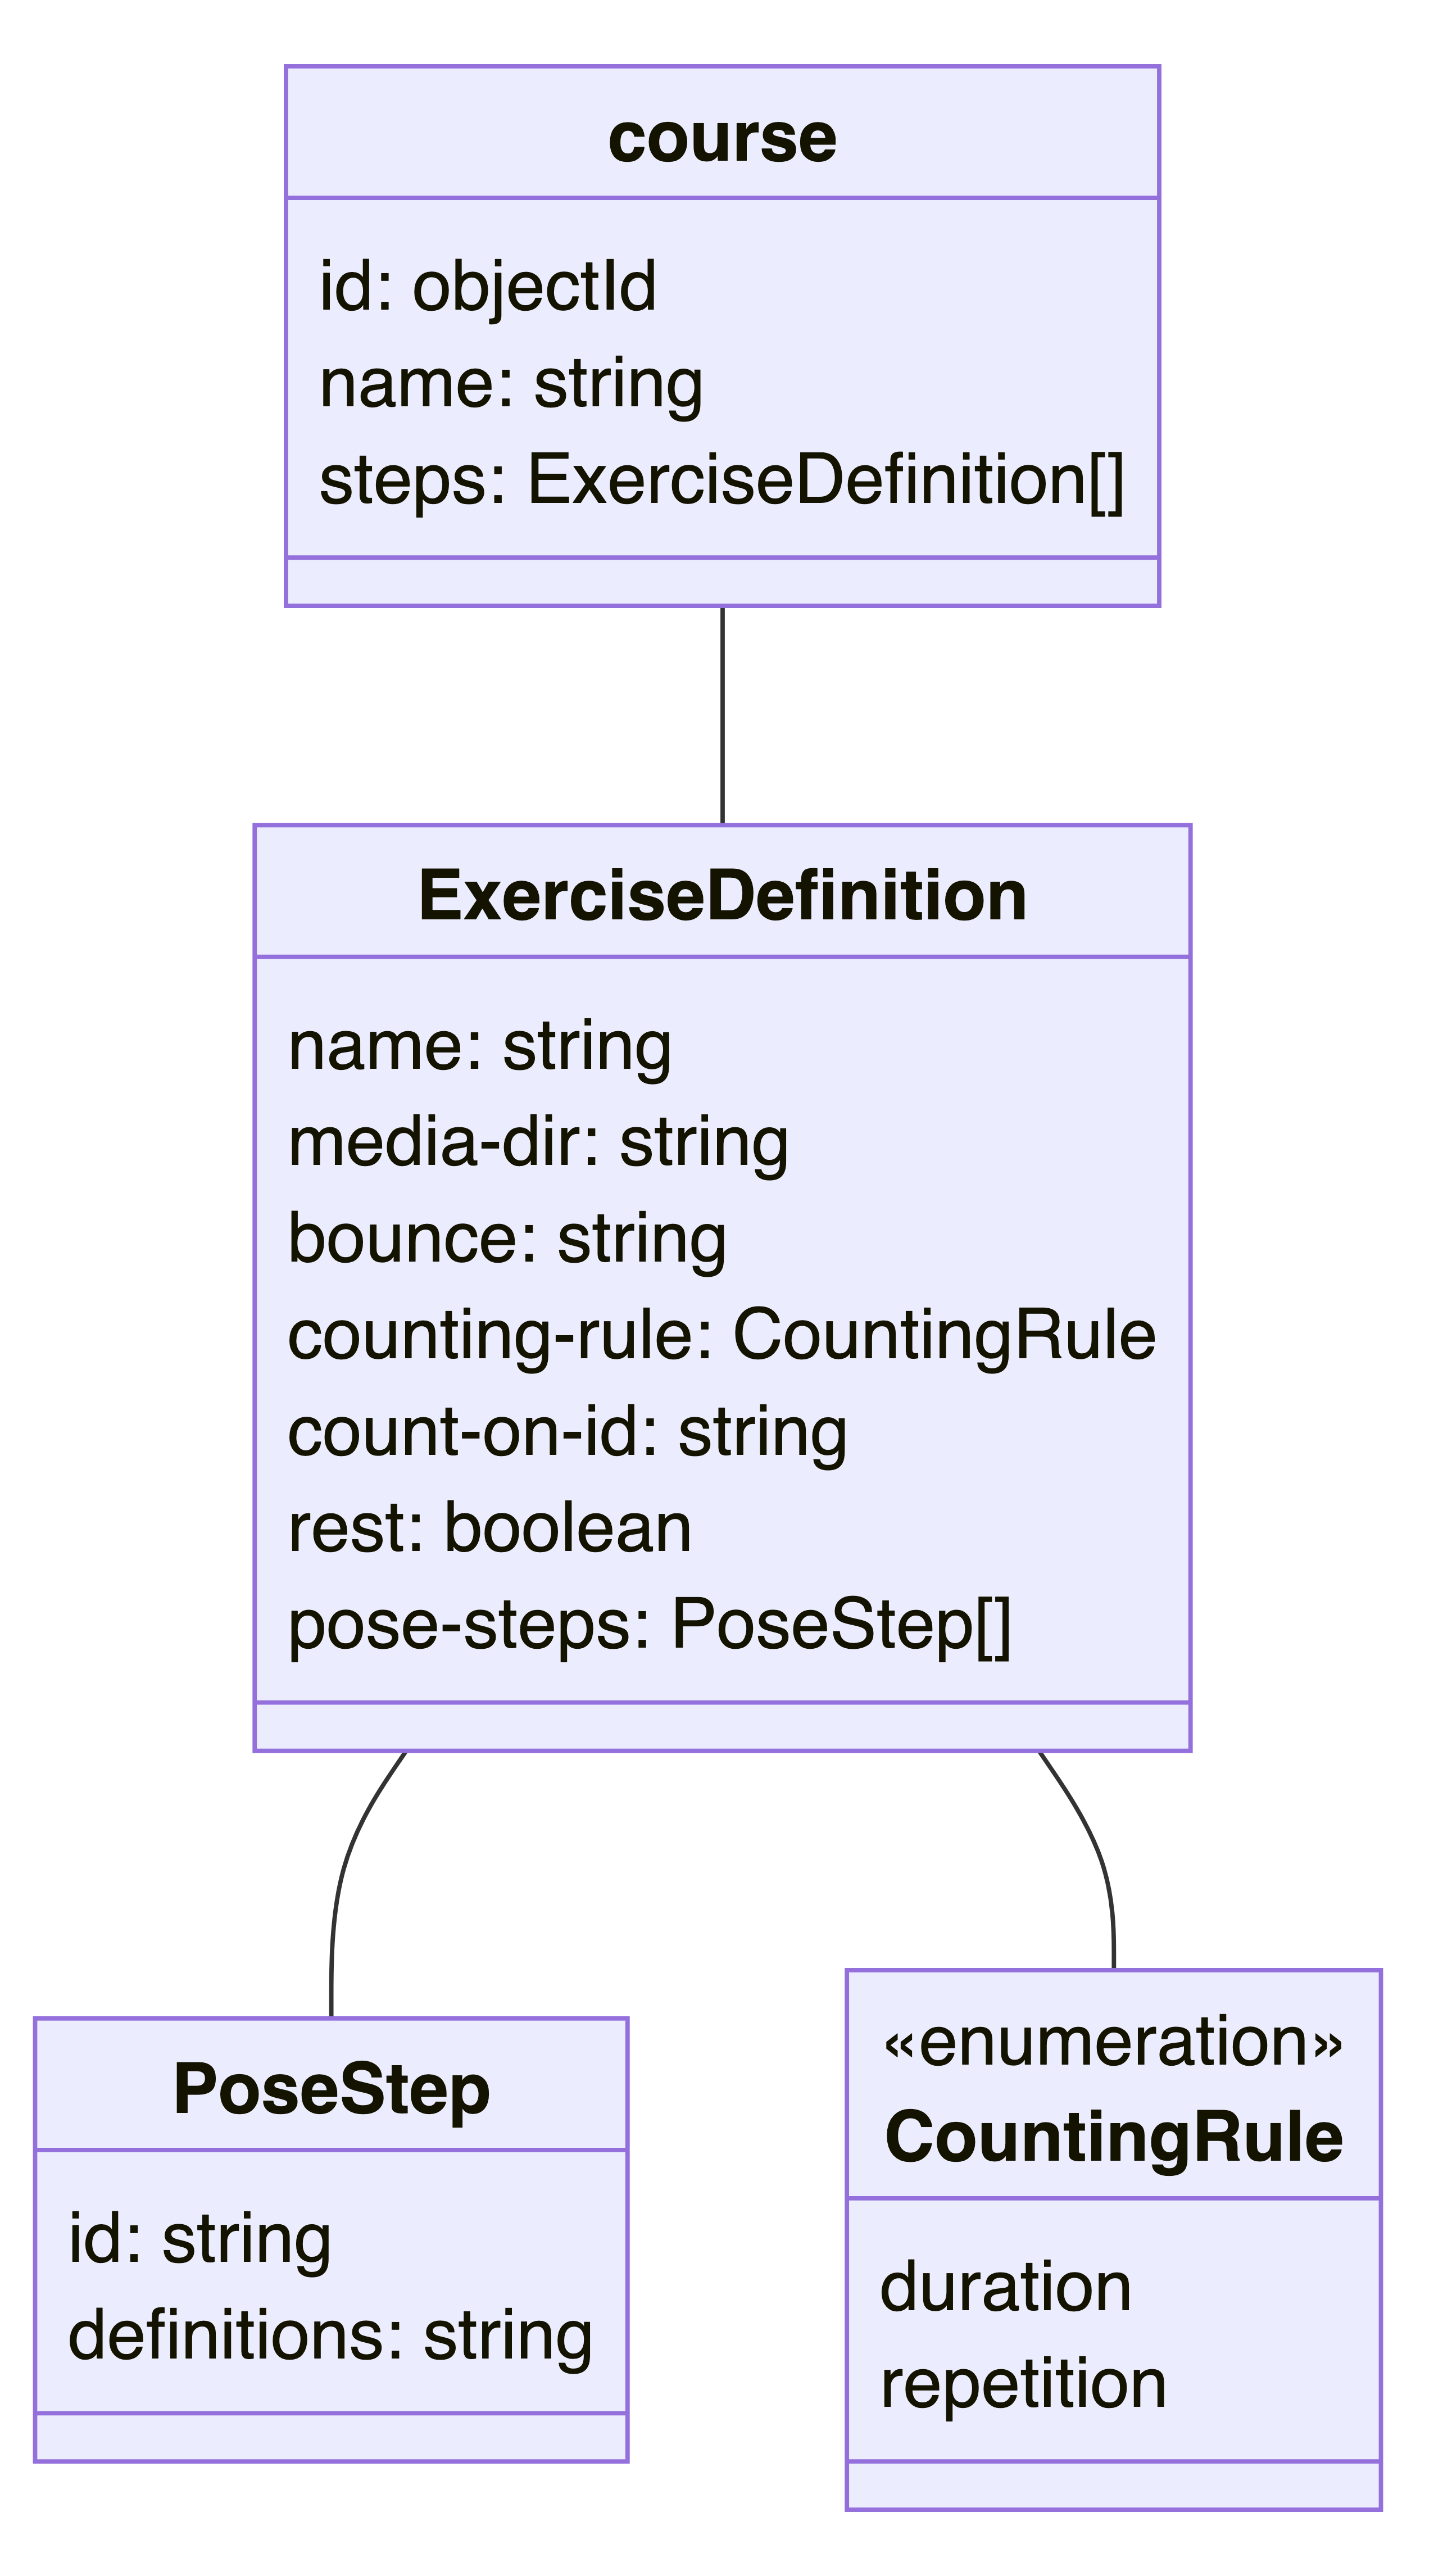
\includegraphics[width=6cm]{chapter_3/course-yaml-1.md.png}
    \caption{UML Class Diagram แสดงโครงสร้างไฟล์ข้อมูลท่าทาง}
\end{figure}

จากโครงสร้างไฟล์ จะมีรายละเอียดต่าง ๆ ในคลาส course ดังนี้
\begin{enumerate}
    \item id: ID ของคอร์ส
    \item name: ชื่อคอร์ส
    \item step: จะเป็นอาเรย์ใช้ในการเก็บข้อมูลท่าทางการออกกำลังกายทั้งหมด รวมถึงลำดับของท่าทางของการออกกำลังกายในคอร์ส ซึ่งจะใช้เก็บข้อมูลของคลาส ExerciseDefinition
\end{enumerate}

รายละเอียดของคลาส ExerciseDefinition มีดังนี้
\begin{enumerate}
    \item name: ชื่อท่าทาง
    \item media-dir: ที่อยู่ของสื่อที่จะนำมาใช้สอนผู้ใช้
    \item bounce: เป็นการกำหนดว่าท่าทางนี้เป็นแบบไป-กลับ หรือไม่ เช่น ในท่าทางวิดพื้นจะต้องมีการงอศอกลงและขึ้น ซึ่งจะต้องกำหนดให้เป็นท่าทางแบบไป-กลับ
    \item counting-rule: เป็นการกำหนดว่าจะใช้วิธีการนับแบบใด ซึ่งจะสามารถเลือกกำหนดได้ ระหว่างการจับเวลาหรือการนับการกระทำซ้ำ
    \item count-on-id: เป็นการกำหนด ID ของท่าทางย่อย ที่เมื่อผู้ใช้ทำท่าทางนี้สำเร็จจะให้นับจำนวนขึ้น ใช้ในกรณีที่ counting-rule ถูกกำหนดเป็นแบบการกระทำซ้ำเท่านั้น
    \item rest: ใช้กำหนดว่าในท่าทางนี้จะเป็นการพักหรือไม่ ถ้ากำหนดเป็น true ระบบจะไม่ทำการตรวจสอบท่าทางของผู้ใช้ เพื่อให้ผู้ใช้ได้พัก และจะไม่สนใจข้อมูลอื่น ๆ ที่ถูกกำหนด
    \item pose-steps: อาเรย์ที่ใช้อธิบายท่าทางย่อยในการออกกำลังกายนั้น ๆ
\end{enumerate}

รายละเอียดของคลาส PoseStep มีดังนี้
\begin{enumerate}
    \item id: ID ที่สามารถกำหนดได้อิสระ เพื่อใช้อ้างอิงถึงท่าทางนี้ใน count-on-id
    \item definitions: เกณฑ์ต่าง ๆ ที่จะต้องตรวจสอบในท่าทางย่อย ๆ นี้
\end{enumerate}
จากรายละเอียดข้างต้นในคลาส ExerciseDefinition จะมีการเก็บท่าทางย่อยใน key ชื่อ pose-steps ซึ่งในระบบจะมองว่าท่าทางการออกกำลังกายจะประกอบไปด้วยท่าทางย่อย ๆ ที่ต้องทำ เช่น ในการออกกำลังกายวิดพื้น จะมีท่าทางย่อย 2 ท่าทาง คือท่าทางเริ่มต้น และท่าทางเมื่องอศอก เป็นต้น โดยลำดับของท่าย่อย ๆ จะอ้างอิงตามลำดับในอาเรย์ ซึ่งถ้ามีการกำหนดให้ท่าทางนี้เป็นแบบไป-กลับ ระบบจะทราบว่าในท่าทางย่อย ๆ นี้เมื่อถึงท่าทางย่อยลำดับสุดท้ายแล้วผู้ใช้ต้องทำท่าทางย้อนกลับ

ในส่วนของคลาส PoseStep จะมี key ชื่อ definitions ซึ่งจะเป็น string ที่ใช้เก็บเกณฑ์ต่าง ๆ ที่จะต้องตรวจสอบในท่าทางย่อย ซึ่งจะมีคำสั่งดังนี้

\begin{enumerate}
    \item คำสั่ง “angle” เป็นคำสั่งตรวจสอบองศาของจุดที่ทำมุมกัน โดยจะมีการใช้งานดังนี้
    \begin{lstlisting}[caption=คำสั่ง angle]
        angle landmarkA landmarkB landmarkC {==|>|<|>=|<=|between|!between} angleA [angleB]
    \end{lstlisting}
    \indent ในคำสั่งนี้ ในขั้นแรกจะรับ Argument เข้ามา 3 ตัวซึ่งจะเป็นการระบุชื่อจุด Landmark ซึ่งจะแทนเป็นจุด A, B, C โดยชื่อ Landmark จะอ้างอิงจาก API ของ ML Kit จากนั้นจะเป็นการเลือกตัวดำเนินการว่าต้องการตรวจสอบองศาอย่างไร ซึ่งจะมีตัวเลือกเท่ากับ, มากกว่า, น้อยกว่า, มากกว่าหรือเท่ากับ, น้อยกว่าหรือเท่ากับ, อยู่ระหว่าง และไม่อยู่ระหว่าง และใน Argument สุดท้ายจะรับองศาที่ต้องการให้ตรวจสอบ ถ้าตัวดำเนินการได้ใช้เป็นแบบอยู่ระหว่างหรือไม่อยู่ระหว่าง จะต้องรับ Argument เพิ่มขึ้นมา ทำให้ต้องรับค่าองศา 2 ตัว เพื่อกำหนดขอบเขตองศาที่อยู่ระหว่างกัน
    \item คำสั่ง “touch” ซึ่งเป็นคำสั่งที่ใช้ในการตรวจสอบว่าจุด Landmark สองจุดอยู่ใกล้กันหรือไม่ โดยจะมีการใช้งาน ดังนี้
    \begin{lstlisting}[caption=คำสั่ง touch]
        touch landmarkA landmarkB
    \end{lstlisting}
    ในคำสั่งนี้จะรับ Argument เข้ามา 2 ตัว เป็นชื่อ Landmark ทั้งสองจุดที่ต้องการตรวจสอบ โดยชื่อ Landmark จะอ้างอิงจาก API ของ ML Kit
\end{enumerate}

\subsection{ส่วนการแนะนำท่าทางให้แก่ผู้ใช้}
เมื่อส่วนอัลกอริทึมการตรวจสอบท่าทางของผู้ใช้ ได้ประมวลผลท่าทางเรียบร้อยแล้ว ระบบจะส่งผลการตรวจสอบมายังส่วนการแนะนำท่าทางผู้ใช้ โดยจะทำการแปลงข้อมูลการตรวจสอบที่ได้ เป็นประโยคแนะนำท่าทางภาษาอังกฤษ เพื่อให้ผู้ใช้สามารถเข้าใจได้ง่าย และจะส่งผลลัพธ์การแนะนำท่าทางไปยังส่วนประสานงานผู้ใช้ เพื่อแสดงผลต่อไป

\section{การออกแบบหลักการคำนวณคะแนนความถูกต้องของท่าทางผู้ใช้}
การคำนวณคะแนนท่าทางของผู้ใช้ จะออกมาในรูปแบบเปอร์เซ็นความถูกต้องเฉลี่ยของท่าทางทั้งหมด ซึ่งจะหาได้จากสมการดังนี้ โดยกำหนดให้ $n$ คือจำนวนท่าทางในคอร์สทั้งหมด
\begin{equation}
    score_{course} = \frac{\sum_{i=1}^{n}{score_{pose_i}}}{n}
\end{equation}
และในแต่ละท่าทางการออกกำลังกาย จะสามารถคำนวณความถูกต้องได้จากเกณฑ์ต่าง ๆ ที่ตรวจสอบ ซึ่งถ้ามีเกณฑ์ใด ๆ จากท่าทางย่อยที่ไม่ตรงตามเกณฑ์ จะถือว่าท่าทางย่อยนั้นไม่ถูกต้อง ซึ่งการคำนวณเปอร์เซ็นต์ความถูกต้องจะนำท่าทางย่อยที่ถูกต้องหารกับท่าทางย่อยที่ได้ทำทั้งหมดซึ่งจะรวมไปถึงท่าทางที่ผิด จะเขียนเป็นสมการได้ ดังนี้
\begin{equation}
    score_{exercise pose} = \frac{correct subpose}{all subpose}
\end{equation}


